\documentclass{article}
\pdfoutput=1

% header.tex
% this is where you load pacakges, specify custom formats, etc.
\pdfoutput=1

% added by Nancy for colour comments
\usepackage{xcolor}

% \usepackage{changepage}
\usepackage{mathtools}
\usepackage{bbm}
% enumitem for custom lists
\usepackage{enumitem}
% Load dsfont this to get proper indicator function (bold 1) with \mathds{1}:
\usepackage{dsfont}
%\usepackage{centernot}
\usepackage{appendix}
\usepackage{multirow}
\usepackage{subcaption}

\usepackage{pdfpages}
\usepackage{arxiv}
\usepackage{natbib}
\usepackage{latexsym}
\usepackage{amsmath}
\usepackage{amsfonts}
\usepackage{amsthm}
\usepackage{amssymb}
\usepackage{psfrag}
\usepackage{graphicx}
\usepackage{url}
\usepackage{enumitem}
\usepackage{algorithm}
\usepackage{algpseudocode}

\bibliographystyle{apalike}

% set up graphics
\usepackage{graphicx}
\DeclareGraphicsExtensions{.pdf,.png,.jpg}
\graphicspath{ {fig/} }
% defs.tex
% this is where you define custom notation, commands, etc.
\pdfoutput=1

\DeclareMathOperator*{\argmax}{arg\,max}
\DeclareMathOperator*{\argmin}{arg\,min}
\DeclareMathOperator*{\del}{\nabla}
\DeclareMathOperator*{\logit}{logit}

%%
% full alphabets of different styles
%%

% personal new commands
\def\delt{\Delta t}
\def\Z{\tilde{Y}^*}
\def\Zone{\tilde{A}^*}
\def\Ztwo{\tilde{W}^*}
\def\z{\tilde{y}^*}
\def\zone{\tilde{a}^*}
\def\ztwo{\tilde{w}^*}

\def\Ya{\bar{Y}}
\def\ya{\bar{y}}
\def\fa{\bar{f}}
\def\Pa{P}
\def\thetaa{\bar{\theta}}

% bf series
\def\bfA{\mathbf{A}}
\def\bfB{\mathbf{B}}
\def\bfC{\mathbf{C}}
\def\bfD{\mathbf{D}}
\def\bfE{\mathbf{E}}
\def\bfF{\mathbf{F}}
\def\bfG{\mathbf{G}}
\def\bfH{\mathbf{H}}
\def\bfI{\mathbf{I}}
\def\bfJ{\mathbf{J}}
\def\bfK{\mathbf{K}}
\def\bfL{\mathbf{L}}
\def\bfM{\mathbf{M}}
\def\bfN{\mathbf{N}}
\def\bfO{\mathbf{O}}
\def\bfP{\mathbf{P}}
\def\bfQ{\mathbf{Q}}
\def\bfR{\mathbf{R}}
\def\bfS{\mathbf{S}}
\def\bfT{\mathbf{T}}
\def\bfU{\mathbf{U}}
\def\bfV{\mathbf{V}}
\def\bfW{\mathbf{W}}
\def\bfX{\mathbf{X}}
\def\bfY{\mathbf{Y}}
\def\bfZ{\mathbf{Z}}

\def\bfa{\mathbf{a}}
\def\bfb{\mathbf{b}}
\def\bfc{\mathbf{c}}
\def\bfd{\mathbf{d}}
\def\bfe{\mathbf{e}}
\def\bff{\mathbf{f}}
\def\bfg{\mathbf{g}}
\def\bfh{\mathbf{h}}
\def\bfi{\mathbf{i}}
\def\bfj{\mathbf{j}}
\def\bfk{\mathbf{k}}
\def\bfl{\mathbf{l}}
\def\bfm{\mathbf{m}}
\def\bfn{\mathbf{n}}
\def\bfo{\mathbf{o}}
\def\bfp{\mathbf{p}}
\def\bfq{\mathbf{q}}
\def\bfr{\mathbf{r}}
\def\bfs{\mathbf{s}}
\def\bft{\mathbf{t}}
\def\bfu{\mathbf{u}}
\def\bfv{\mathbf{v}}
\def\bfw{\mathbf{w}}
\def\bfx{\mathbf{x}}
\def\bfy{\mathbf{y}}
\def\bfz{\mathbf{z}}

% bb series
\def\bbA{\mathbb{A}}
\def\bbB{\mathbb{B}}
\def\bbC{\mathbb{C}}
\def\bbD{\mathbb{D}}
\def\bbE{\mathbb{E}}
\def\bbF{\mathbb{F}}
\def\bbG{\mathbb{G}}
\def\bbH{\mathbb{H}}
\def\bbI{\mathbb{I}}
\def\bbJ{\mathbb{J}}
\def\bbK{\mathbb{K}}
\def\bbL{\mathbb{L}}
\def\bbM{\mathbb{M}}
\def\bbN{\mathbb{N}}
\def\bbO{\mathbb{O}}
\def\bbP{\mathbb{P}}
\def\bbQ{\mathbb{Q}}
\def\bbR{\mathbb{R}}
\def\bbS{\mathbb{S}}
\def\bbT{\mathbb{T}}
\def\bbU{\mathbb{U}}
\def\bbV{\mathbb{V}}
\def\bbW{\mathbb{W}}
\def\bbX{\mathbb{X}}
\def\bbY{\mathbb{Y}}
\def\bbZ{\mathbb{Z}}

% cal series
\def\calA{\mathcal{A}}
\def\calB{\mathcal{B}}
\def\calC{\mathcal{C}}
\def\calD{\mathcal{D}}
\def\calE{\mathcal{E}}
\def\calF{\mathcal{F}}
\def\calG{\mathcal{G}}
\def\calH{\mathcal{H}}
\def\calI{\mathcal{I}}
\def\calJ{\mathcal{J}}
\def\calK{\mathcal{K}}
\def\calL{\mathcal{L}}
\def\calM{\mathcal{M}}
\def\calN{\mathcal{N}}
\def\calO{\mathcal{O}}
\def\calP{\mathcal{P}}
\def\calQ{\mathcal{Q}}
\def\calR{\mathcal{R}}
\def\calS{\mathcal{S}}
\def\calT{\mathcal{T}}
\def\calU{\mathcal{U}}
\def\calV{\mathcal{V}}
\def\calW{\mathcal{W}}
\def\calX{\mathcal{X}}
\def\calY{\mathcal{Y}}
\def\calZ{\mathcal{Z}}

\def\bfTheta{\mathbf{\Theta}}


%%%%%%%%%%%%%%%%%%%%%%%%%%%%%%%%%%%%%%%%%%%%%%%%%%%%%%%%%%
% text short-cuts
\def\iid{i.i.d.\ } %i.i.d.
\def\ie{i.e.\ }
\def\eg{e.g.\ }
\def\Polya{P\'{o}lya\ }
%%%%%%%%%%%%%%%%%%%%%%%%%%%%%%%%%%%%%%%%%%%%%%%%%%%%%%%%%%

%%%%%%%%%%%%%%%%%%%%%%%%%%%%%%%%%%%%%%%%%%%%%%%%%%%%%%%%%%
% quasi-universal probabilistic and mathematical notation
% my preferences (modulo publication conventions, and clashes like random vectors):
%   vectors: bold, lowercase
%   matrices: bold, uppercase
%   operators: blackboard (e.g., \mathbb{E}), uppercase
%   sets, spaces: calligraphic, uppercase
%   random variables: normal font, uppercase
%   deterministic quantities: normal font, lowercase
%%%%%%%%%%%%%%%%%%%%%%%%%%%%%%%%%%%%%%%%%%%%%%%%%%%%%%%%%%

% operators
\def\P{\bbP} %fundamental probability
\def\E{\bbE} %expectation
% conditional expectation
\DeclarePairedDelimiterX\bigCond[2]{[}{]}{#1 \;\delimsize\vert\; #2}
\newcommand{\conditional}[3][]{\bbE_{#1}\bigCond*{#2}{#3}}
\def\Law{\mathcal{L}} %law; this is by convention in the literature
\def\indicator{\mathds{1}} % indicator function

% sets and groups
\def\borel{\calB} %Borel sets
\def\sigAlg{\calA} %sigma-algebra
\def\filtration{\calF} %filtration
\def\grp{\calG} %group

% binary relations
\def\condind{{\perp\!\!\!\perp}} %independence/conditional independence
\def\equdist{\stackrel{\text{\rm\tiny d}}{=}} %equal in distribution
\def\equas{\stackrel{\text{\rm\tiny a.s.}}{=}} %euqal amost surely
\def\simiid{\sim_{\mbox{\tiny iid}}} %sampled i.i.d

% common vectors and matrices
\def\onevec{\mathbf{1}}
\def\iden{\mathbf{I}} % identity matrix
\def\supp{\text{\rm supp}}

% misc
% floor and ceiling
\DeclarePairedDelimiter{\ceilpair}{\lceil}{\rceil}
\DeclarePairedDelimiter{\floor}{\lfloor}{\rfloor}
\newcommand{\argdot}{{\,\vcenter{\hbox{\tiny$\bullet$}}\,}} %generic argument dot
%%%%%%%%%%%%%%%%%%%%%%%%%%%%%%%%%%%%%%%%%%%%%%%%%%%%%%%%%%

%%%%%%%%%%%%%%%%%%%%%%%%%%%%%%%%%%%%%%%%%%%%%%%%%%%%%%%%%%
%% some distributions
% continuous
\def\UnifDist{\text{\rm Unif}}
\def\BetaDist{\text{\rm Beta}}
\def\ExpDist{\text{\rm Exp}}
\def\GammaDist{\text{\rm Gamma}}
% \def\GenGammaDist{\text{\rm GGa}} %Generalized Gamma

% discrete
\def\BernDist{\text{\rm Bernoulli}}
\def\BinomDist{\text{\rm Binomial}}
\def\PoissonPlus{\text{\rm Poisson}_{+}}
\def\PoissonDist{\text{\rm Poisson}}
\def\NBPlus{\text{\rm NB}_{+}}
\def\NBDist{\text{\rm NB}}
\def\GeomDist{\text{\rm Geom}}
% \def\CRP{\text{\rm CRP}}
% \def\EGP{\text{\rm EGP}}
% \def\MittagLeffler{\text{\rm ML}}
%%%%%%%%%%%%%%%%%%%%%%%%%%%%%%%%%%%%%%%%%%%%%%%%%%%%%%%%%%

%%%%%%%%%%%%%%%%%%%%%%%%%%%%%%%%%%%%%%%%%%%%%%%%%%%%%%%%%%
% Project-specific notation should go here
% (Because it's at the end of the file, it can overwrite anything that came before.)

%e.g.,
\def\Laplacian{\calL}
\def\P{\calP}

% combinatorial objects
\def\perm{\sigma} %fixed permutation
\def\Perm{\Sigma} %random permutation
\def\part{\pi} %fixed partition
\def\Part{\Pi} %random partition



% Typeset Shortcuts
\newcommand{\C}{{\mathbb{C}}}
\newcommand{\F}{{\mathcal{F}}}
\newcommand{\R}{{\mathbb{R}}}
\newcommand{\N}{{\mathbb{N}}}
\newcommand{\Q}{{\mathbb{Q}}}

\newcommand{\statespace}{\mathcal{X}}
\newcommand{\states}{\textbf{x}}
\newcommand{\augstates}{\textbf{z}}
\newcommand{\pis}{\boldsymbol{\pi}}
\newcommand{\rstates}{\textbf{X}}


\newcommand{\Ps}{\textbf{P}}

\newcommand{\K}{{\textbf{K}}}
\newcommand{\Kcomm}{\K^{\textrm{comm}}_n}
\newcommand{\Kexpl}{\K^{\textrm{expl}}}
\newcommand{\KSEO}{\K^{\textrm{SEO}}}
\newcommand{\KDEO}{\K^{\textrm{DEO}}_n}
\newcommand{\Kodd}{\K^{\textrm{odd}}}
\newcommand{\Keven}{\K^{\textrm{even}}}
\newcommand{\Kswap}{\K^{(i,i+1)}}
\newcommand{\KPT}{\K^{\textrm{PT}}_n}

\newcommand{\Rn}{\mathcal{R}_n}
\newcommand{\Tn}{\mathcal{T}_n}
\newcommand{\Bs}{\textbf{B}}
\newcommand{\partition}{\mathcal{P}}

\newcommand{\PSEO}{\mathbb{P}_{\textrm{SEO}}}
\newcommand{\PDEO}{\mathbb{P}_{\textrm{DEO}}}
\newcommand{\ESEO}{\mathbb{E}_{\textrm{SEO}}}
\newcommand{\EDEO}{\mathbb{E}_{\textrm{DEO}}}

\newcommand{\nexpl}{n_\textrm{expl}} 
\newcommand{\nv}{n_\textrm{var}}

\newcommand{\tauSEO}{\tau_{\textrm{SEO}}}
\newcommand{\tauDEO}{\tau_{\textrm{DEO}}}

\newcommand{\punif}{\mathcal{P}_{\textrm{uniform}}}
\newcommand{\popt}{\mathcal{P}_{\textrm{optimal}}}
\newcommand{\A}{\mathcal{A}}

\newcommand{\norm}[1]{\|{#1}\|}
\newcommand{\Norm}[1]{\left\|{#1}\right\|}
\newcommand{\rank}{{\mathrm{rank}}}
\newcommand{\Var}{\mathrm{Var}}
\newcommand{\Bern}{\mathrm{Bern}}
\renewcommand{\P}{\mathbb{P}}
\newcommand{\I}{{\mathbb{I}}}
\newcommand{\eps}{\varepsilon}
\newcommand{\ud}{\textrm{d}}

\newcommand\deq{\stackrel{\scriptscriptstyle d}{=}}

\newtheorem{theorem}{Theorem}
\newtheorem{corollary}{Corollary}
\newtheorem{lemma}{Lemma}
\newtheorem{proposition}{Proposition}
\newtheorem{remark}{Remark}
\newtheorem{example}{Example}

%%%%%%%%%%%%%%%%%%%%%%%%%%%%%%%%%%%%%%%%%%%%%%%%%%%%%%%%%%

%\def\bibfont{\large}
\usepackage{appendix}

\title{Variance-reduced stochastic optimization for hidden Markov models: Supplementary Plots}

\author{
  Evan Sidrow \\
  Department of Statistics\\
  University of British Columbia\\
  Vancouver, Canada \\
  \texttt{evan.sidrow@stat.ubc.ca} \\
}

\begin{document}

\maketitle

The figures in this supplement display the log-likelihood (divided by $T$) of the maximum log-likelihood minus the log-likelihood (divided by $T$) at each epoch of a selected run of each optimization algorithm after 12 hours or 150 epochs (whichever came first) for four data sets of all experiments. For each optimization algorithm and data set, we display the random initialization that resulted in the highest likelihood after 12 hours. The dots on each figure correspond to the likelihood at convergence. Convergence is defined as the point at which the gradient norm of the log-likelihood (divided by $T$) was less than $10^{-2}$. We selected a tolerance of $10^{-2}$ because it was the lowest tolerance that all algorithms regularly converged to within 12 hours. 

\newpage

\begin{figure}
    \centering
    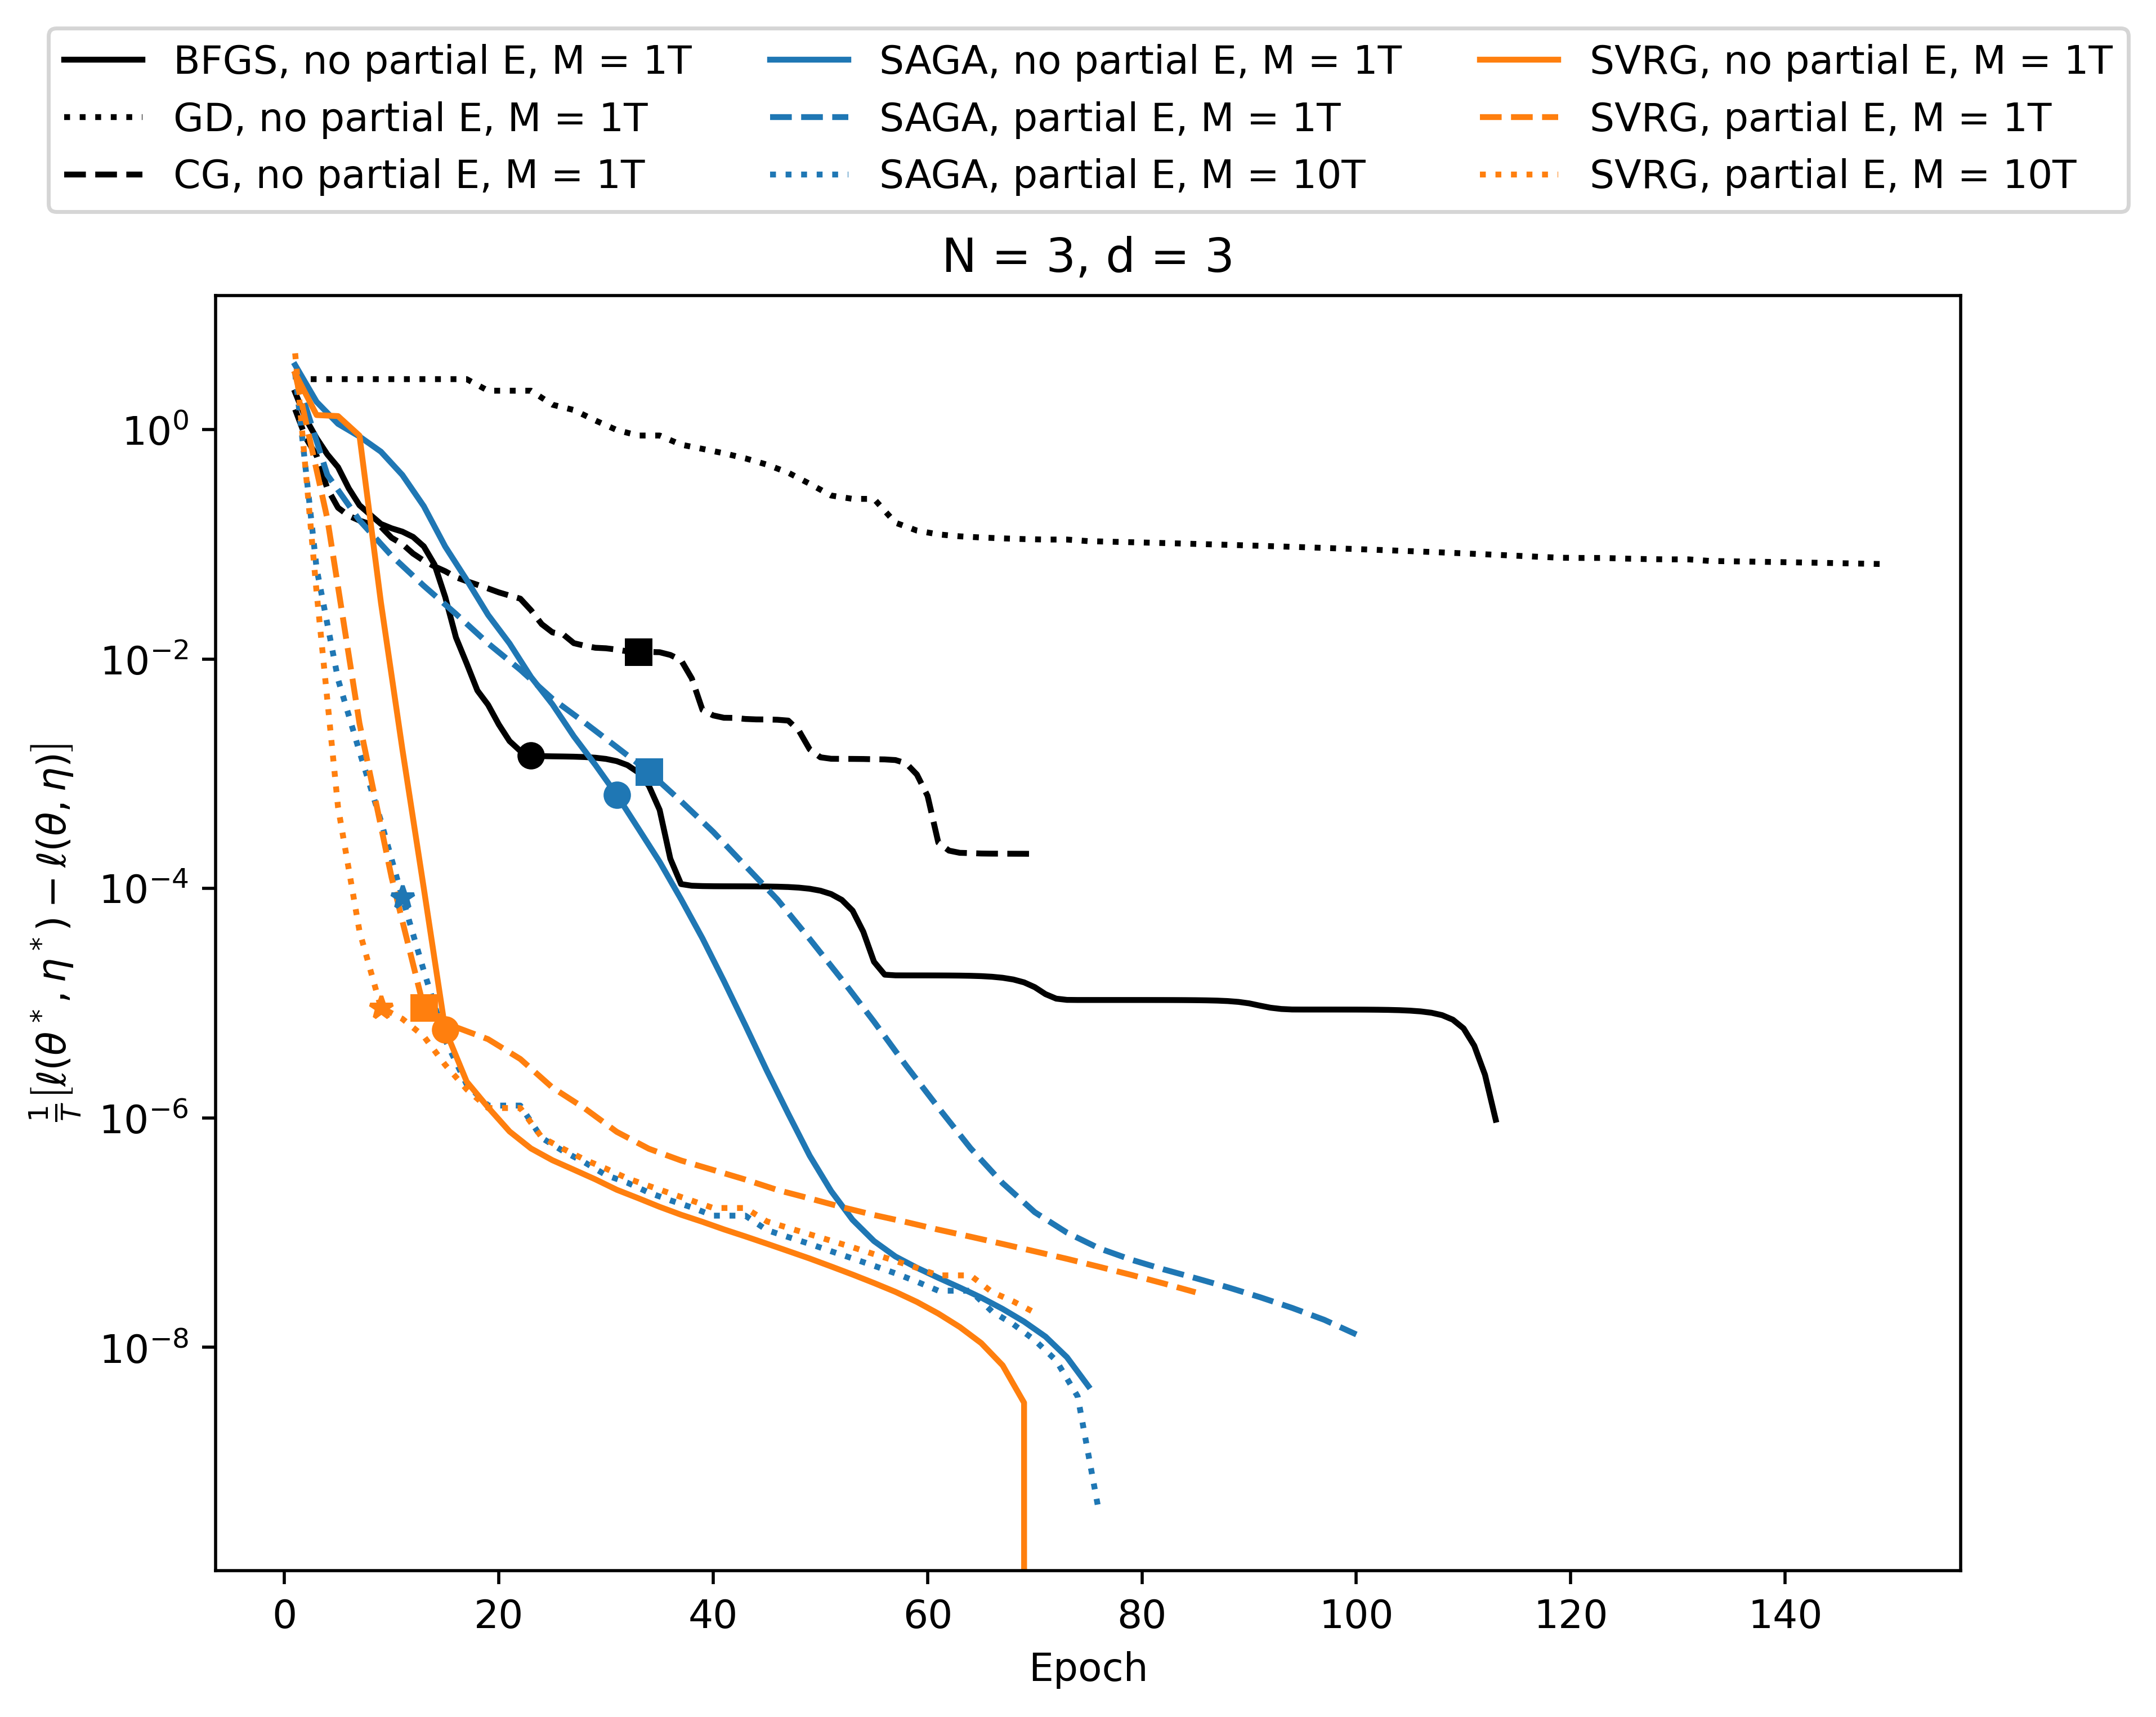
\includegraphics[width=3in]{../plt/log-like_v_epoch_T-100000-K-3-1-d-3-001.png}
    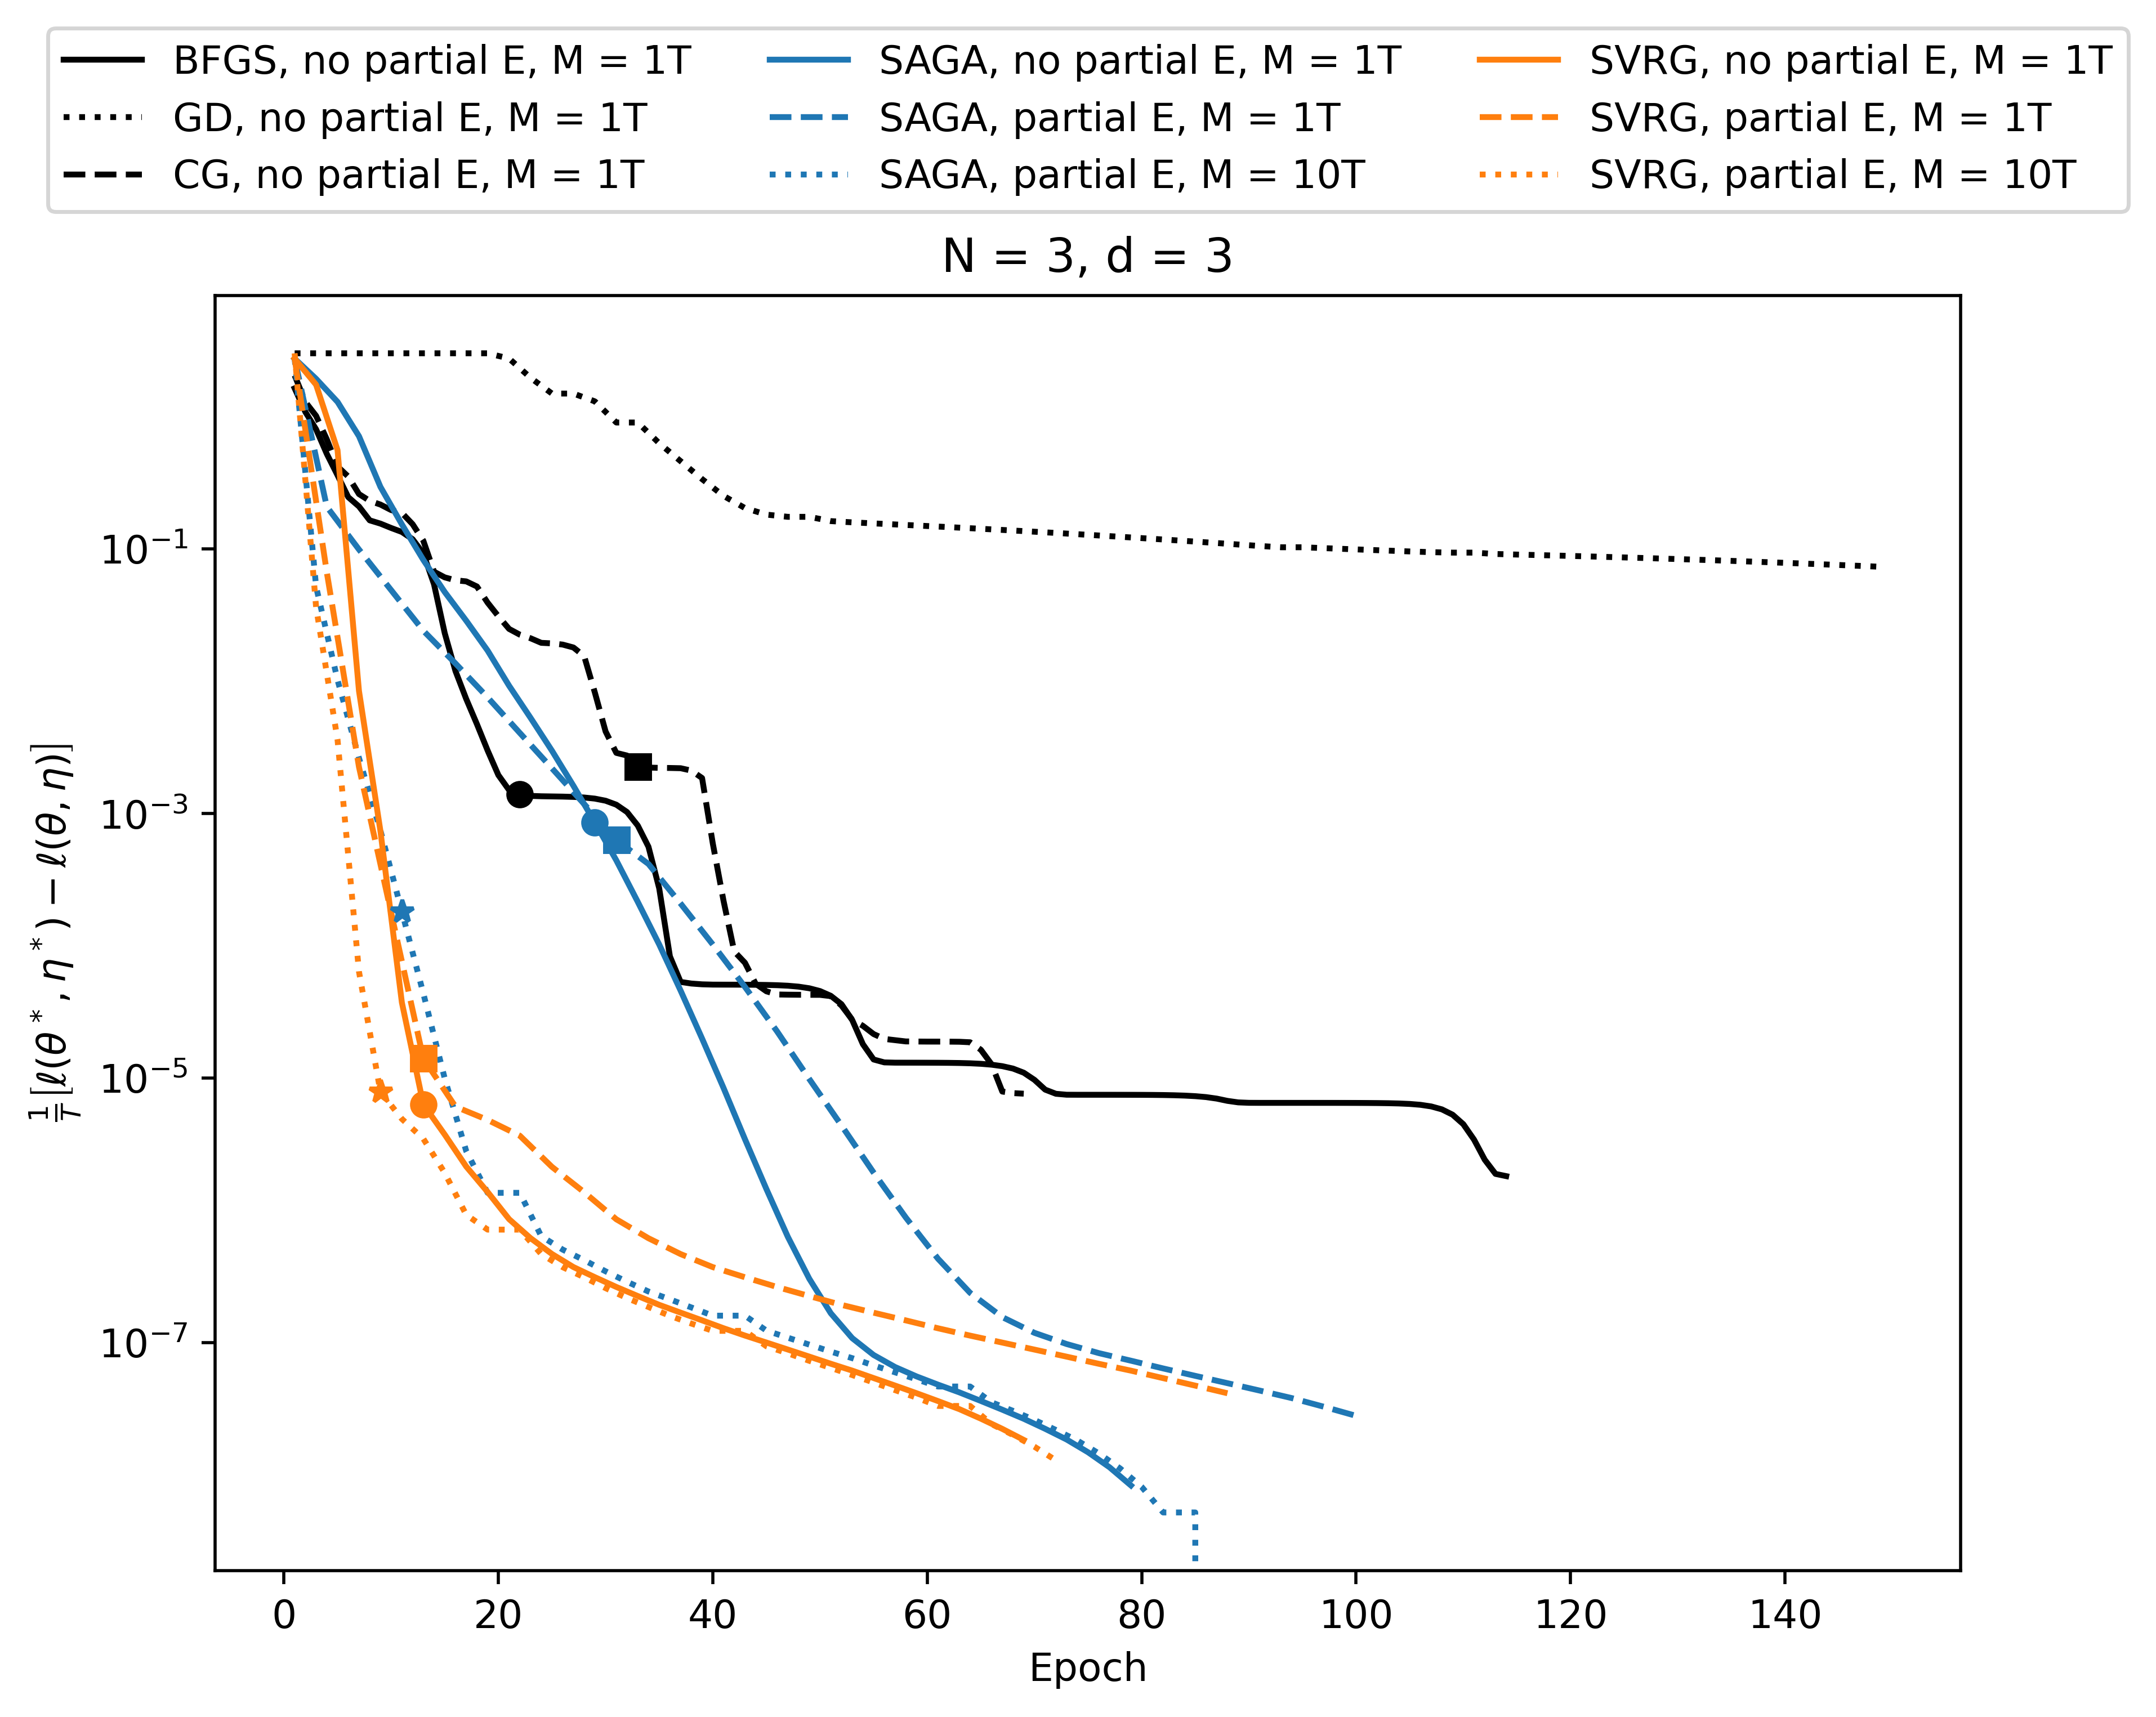
\includegraphics[width=3in]{../plt/log-like_v_epoch_T-100000-K-3-1-d-3-002.png}
    \\
    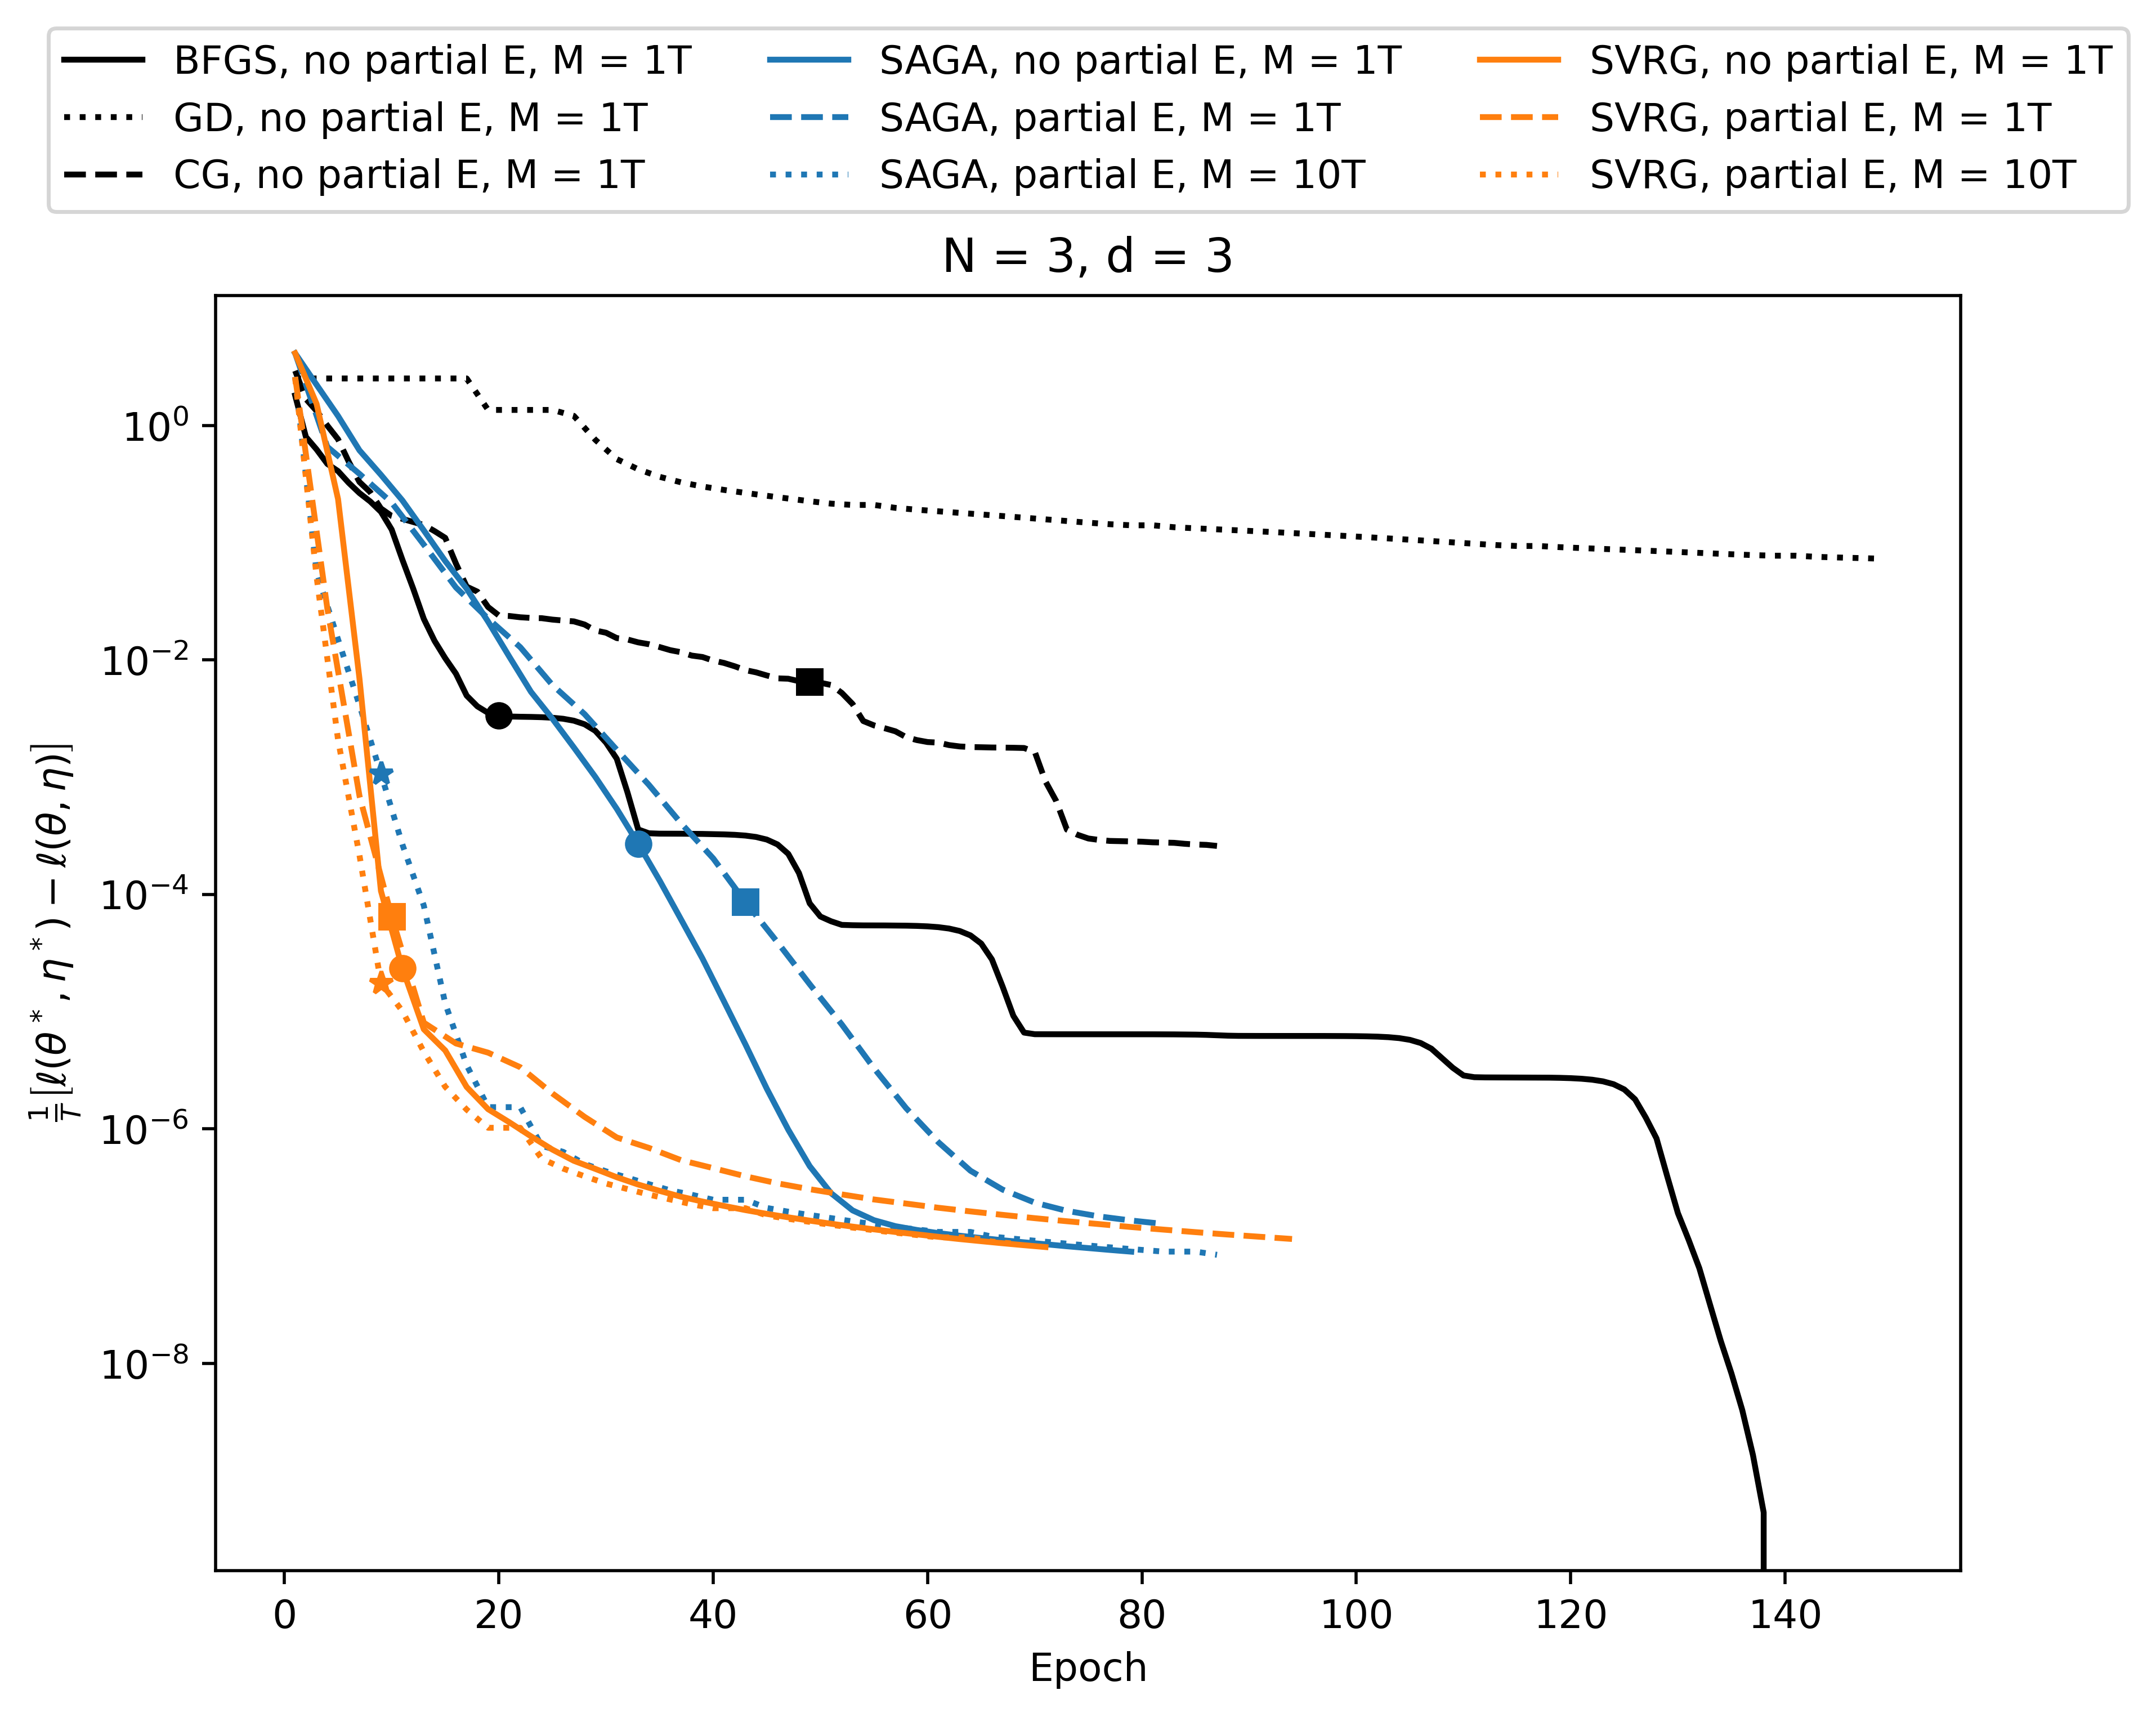
\includegraphics[width=3in]{../plt/log-like_v_epoch_T-100000-K-3-1-d-3-003.png}
    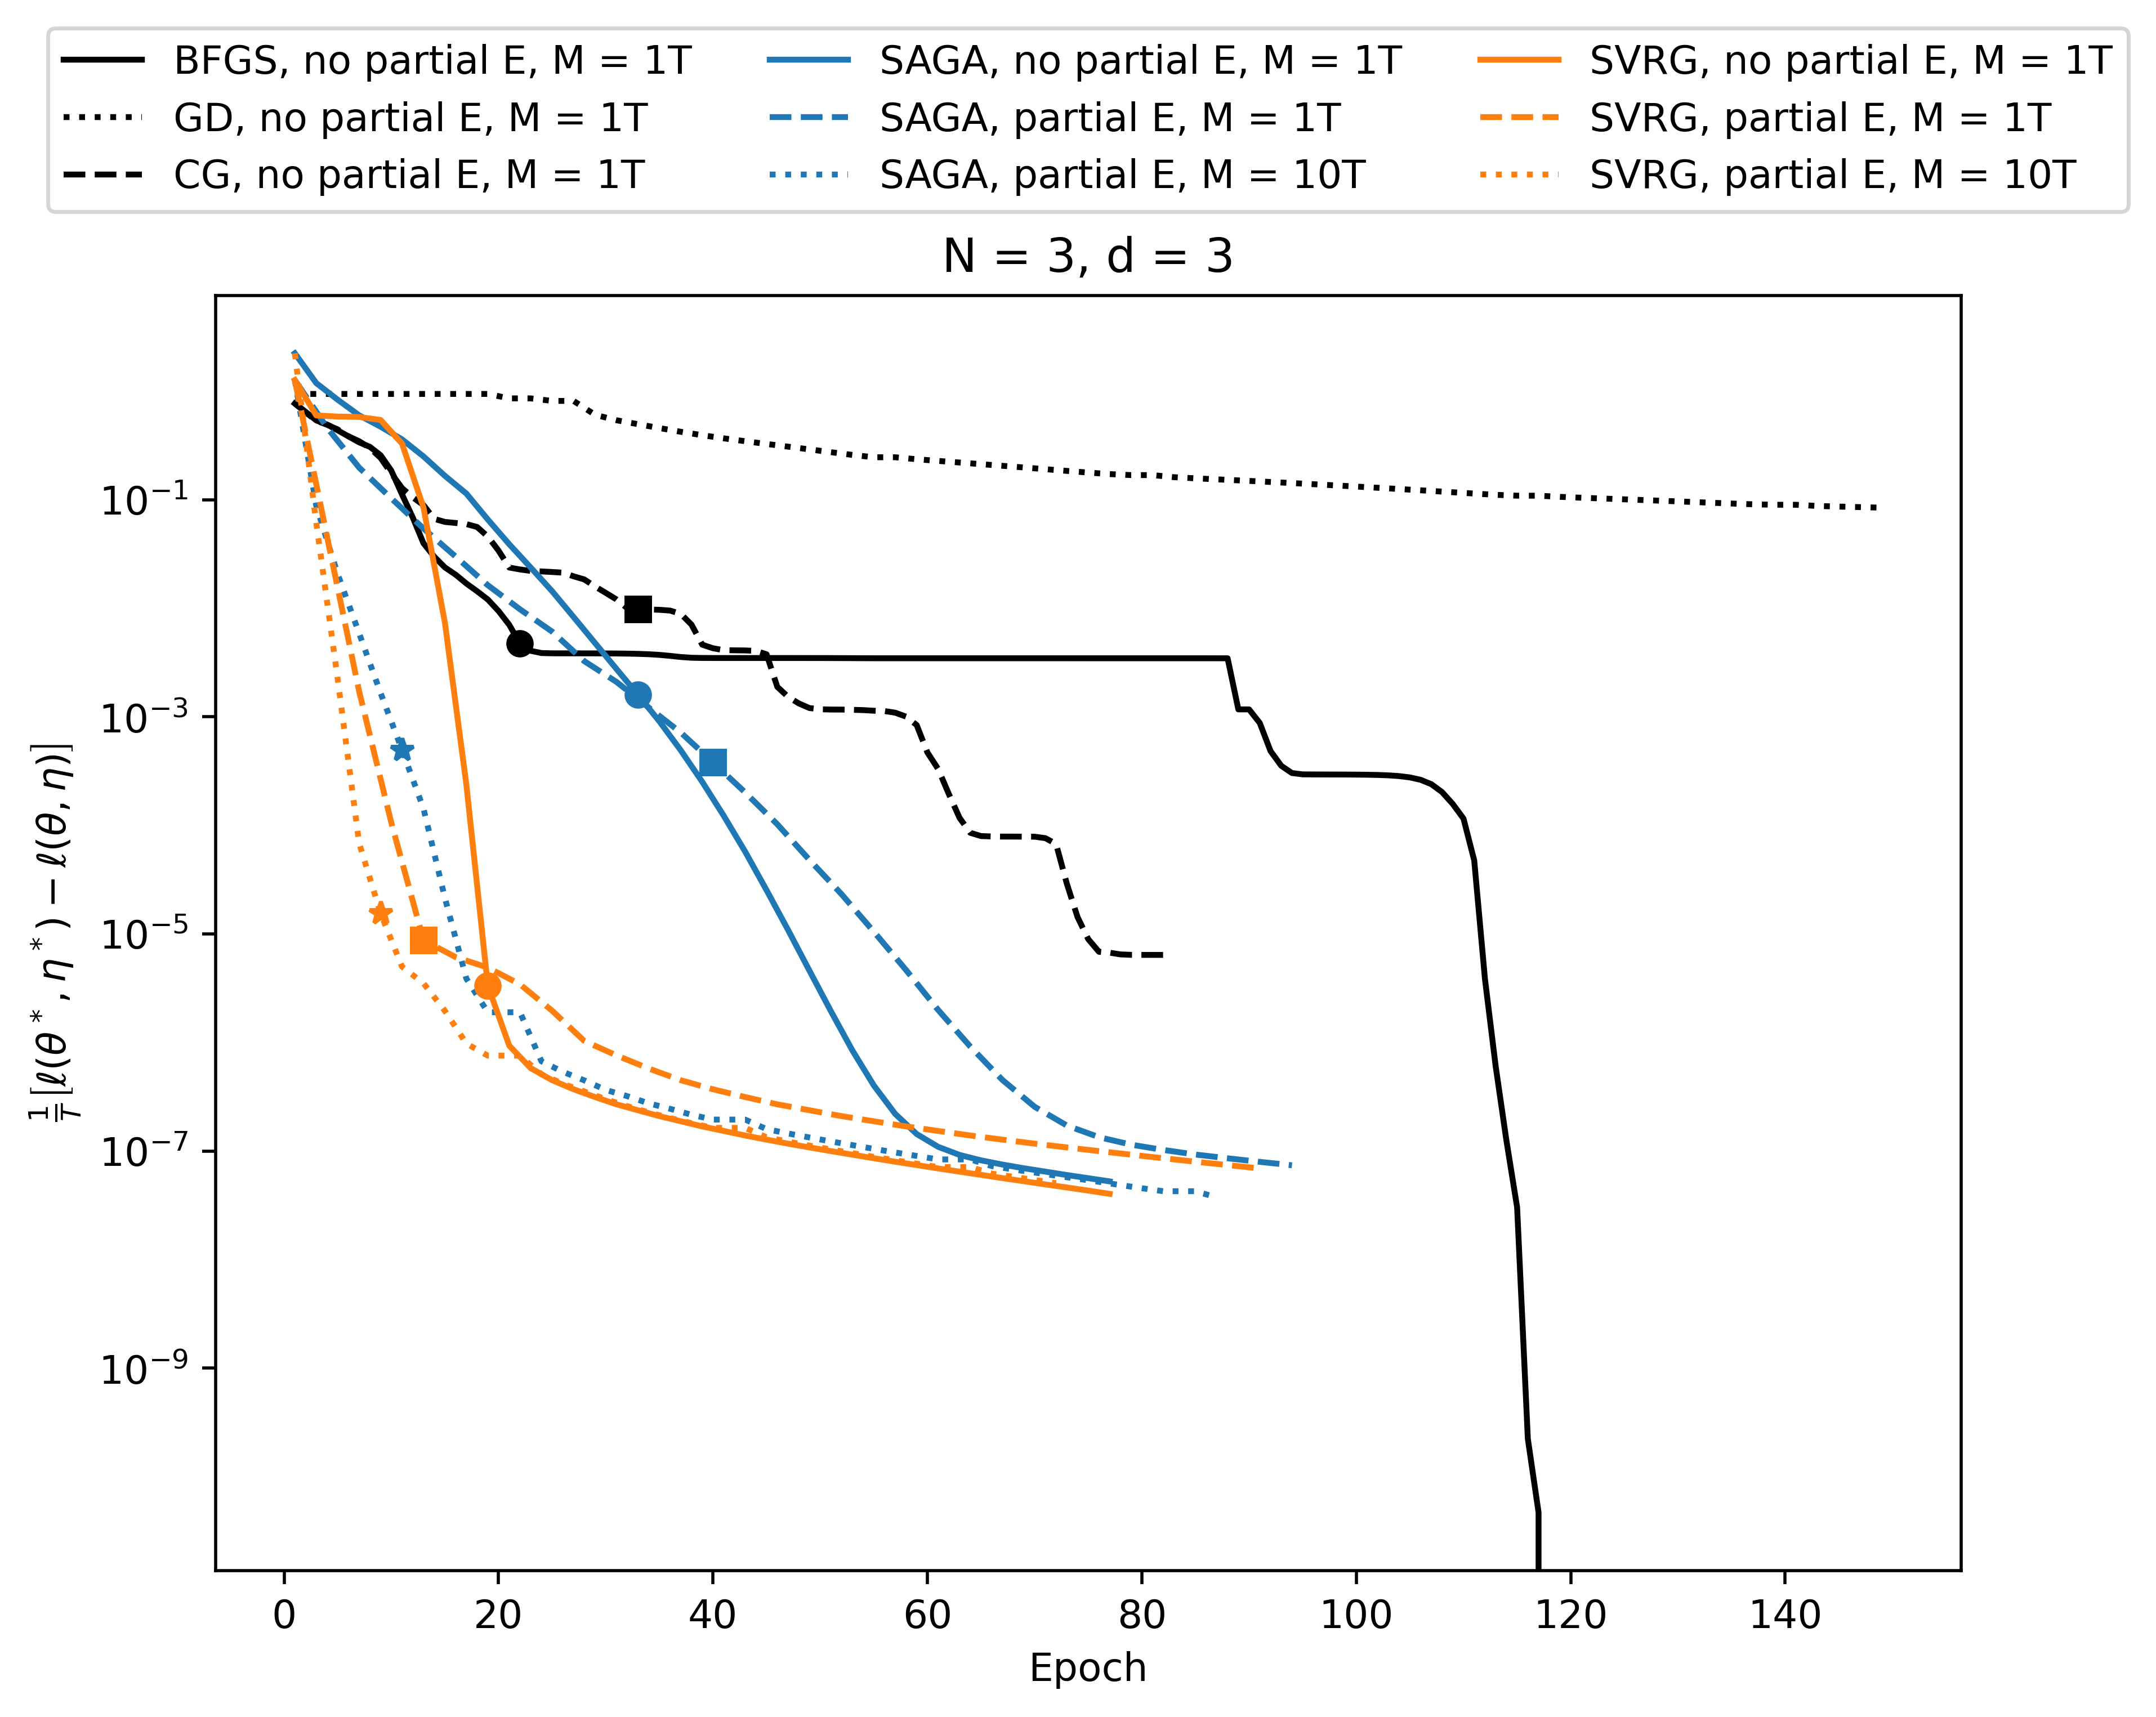
\includegraphics[width=3in]{../plt/log-like_v_epoch_T-100000-K-3-1-d-3-004.png}   
    \caption{Optimally gap between the current log-likelihood and optimal log-likelihood for the simulation studies with $T=10^{5}$, $N=3$ and $d=3$, for four different simulated data sets. One epoch represents either one full E-step, $T$ iterations with the M-step, or one gradient step for full-gradient algorithms. The y-axis is on a log-scale.}
\end{figure}
%
\begin{figure}
    \centering
    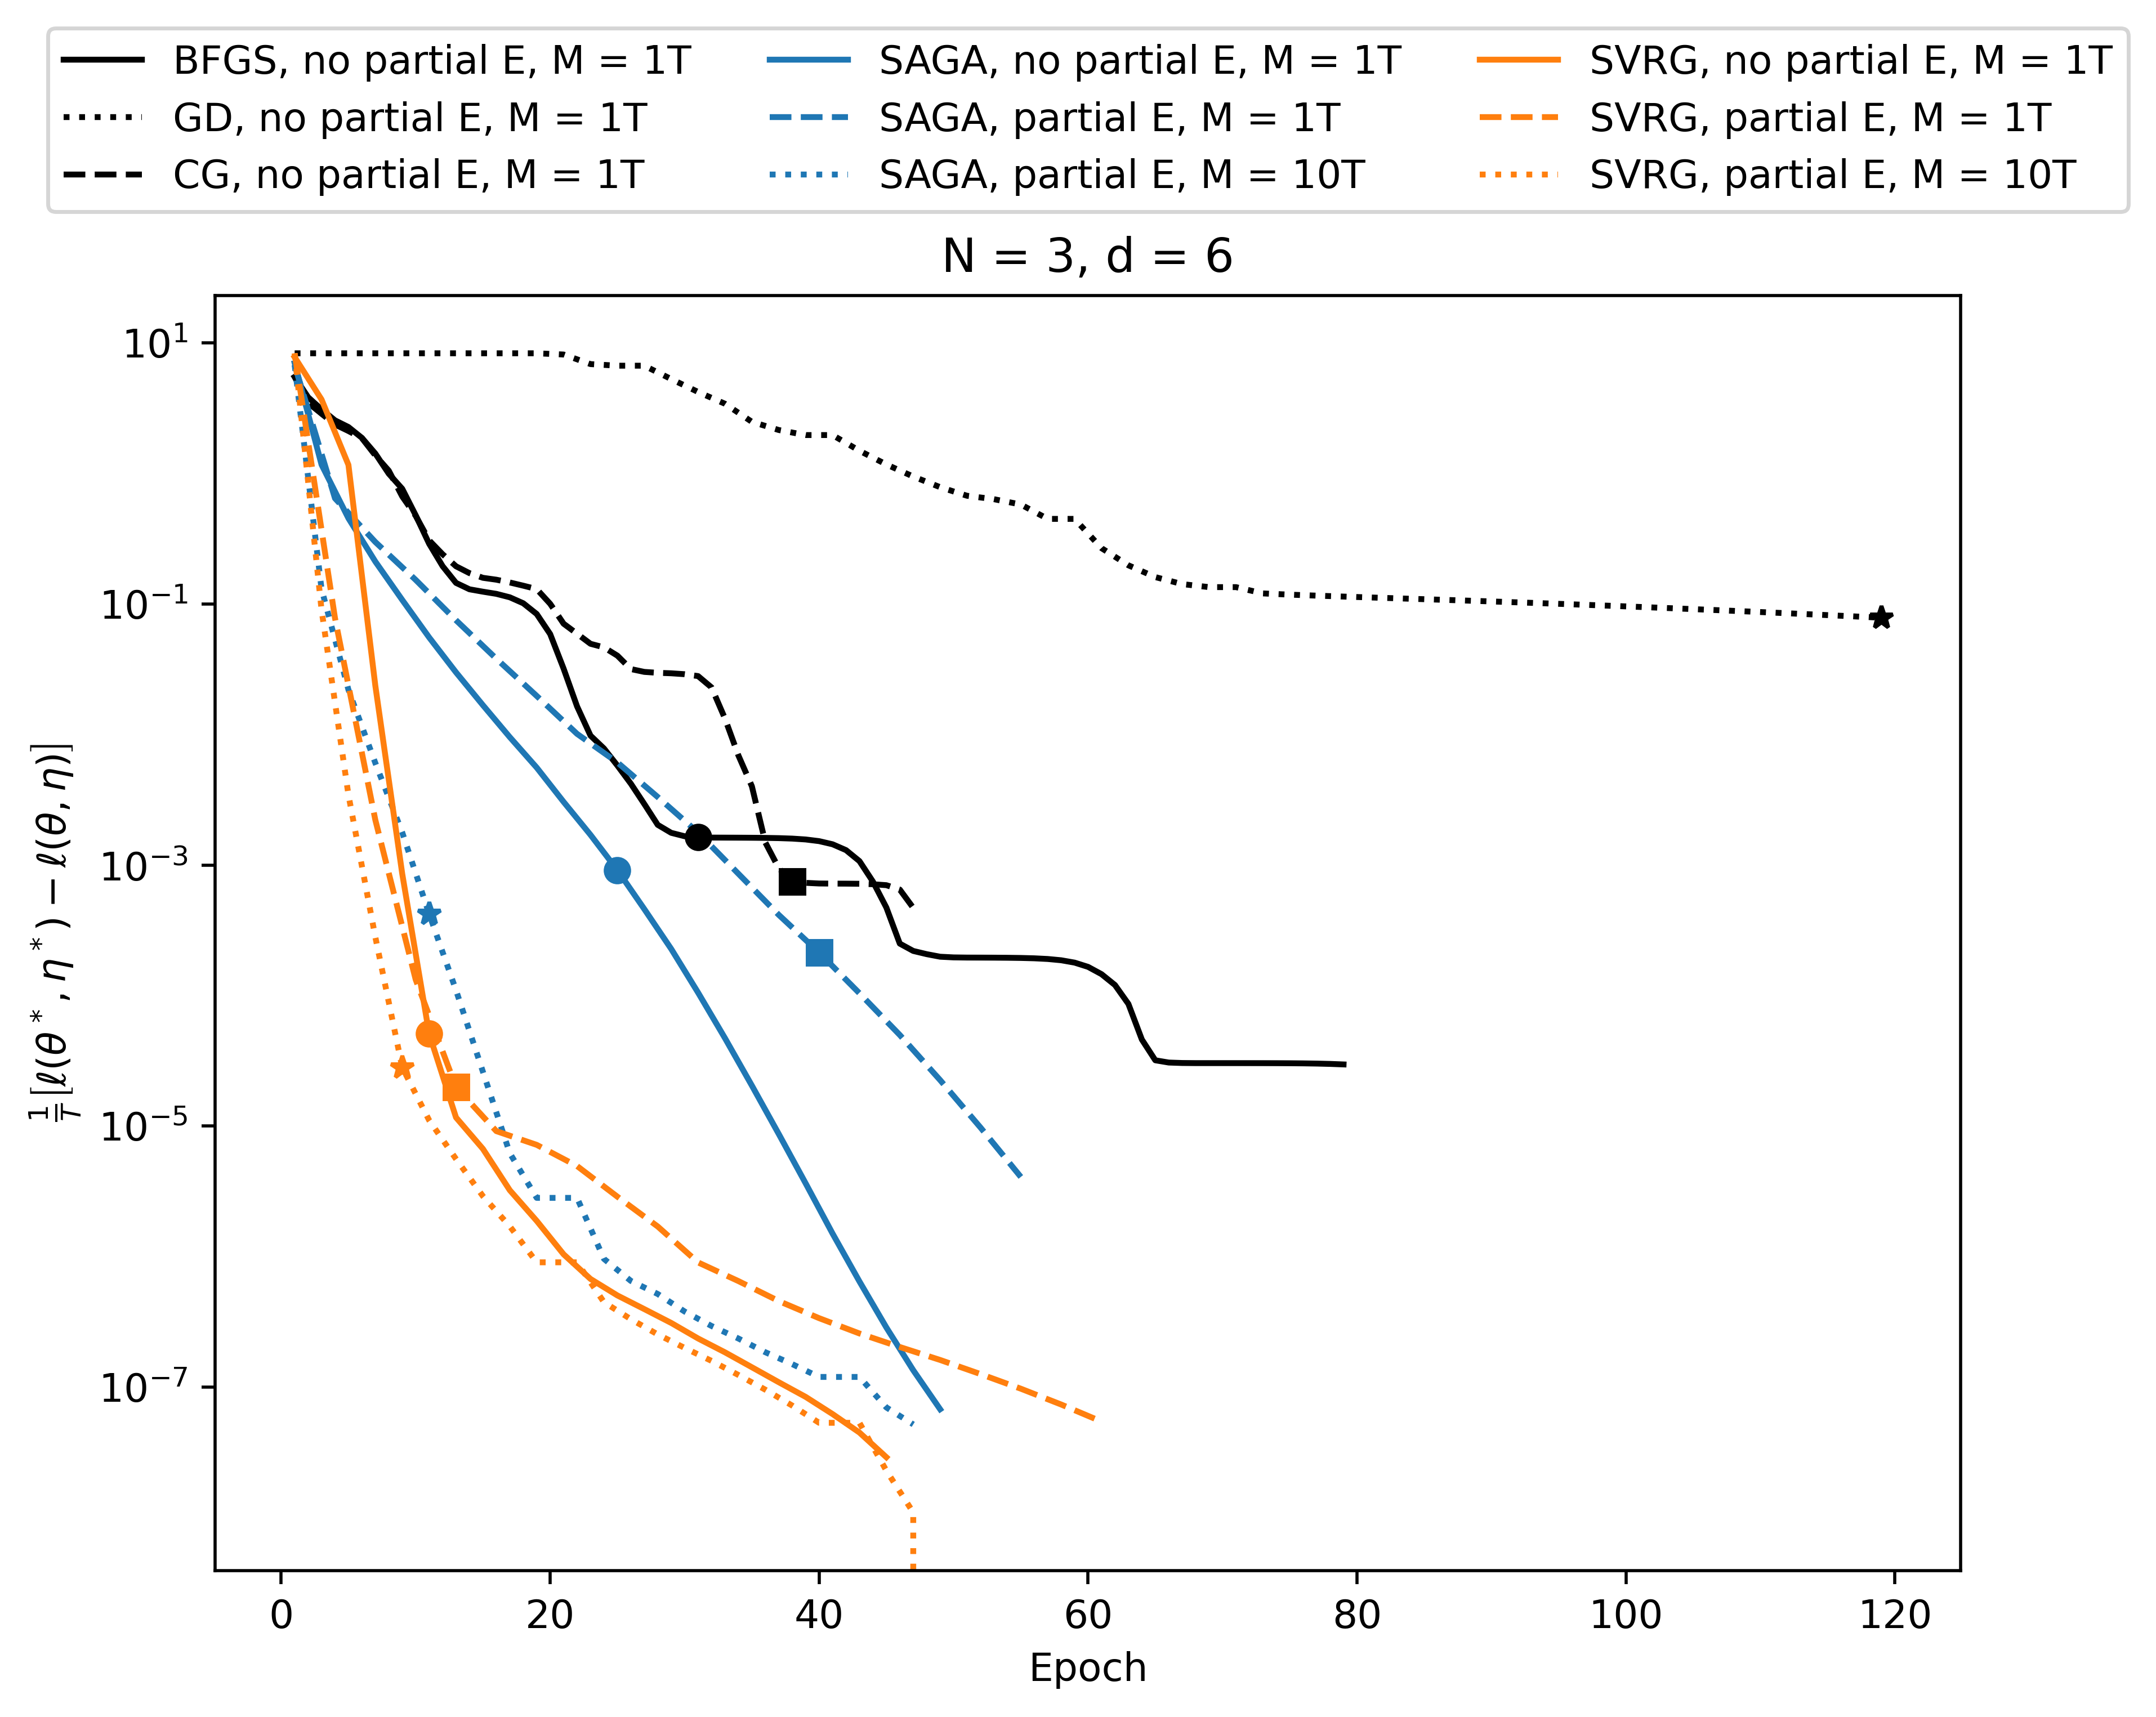
\includegraphics[width=3in]{../plt/log-like_v_epoch_T-100000-K-3-1-d-6-001.png}
    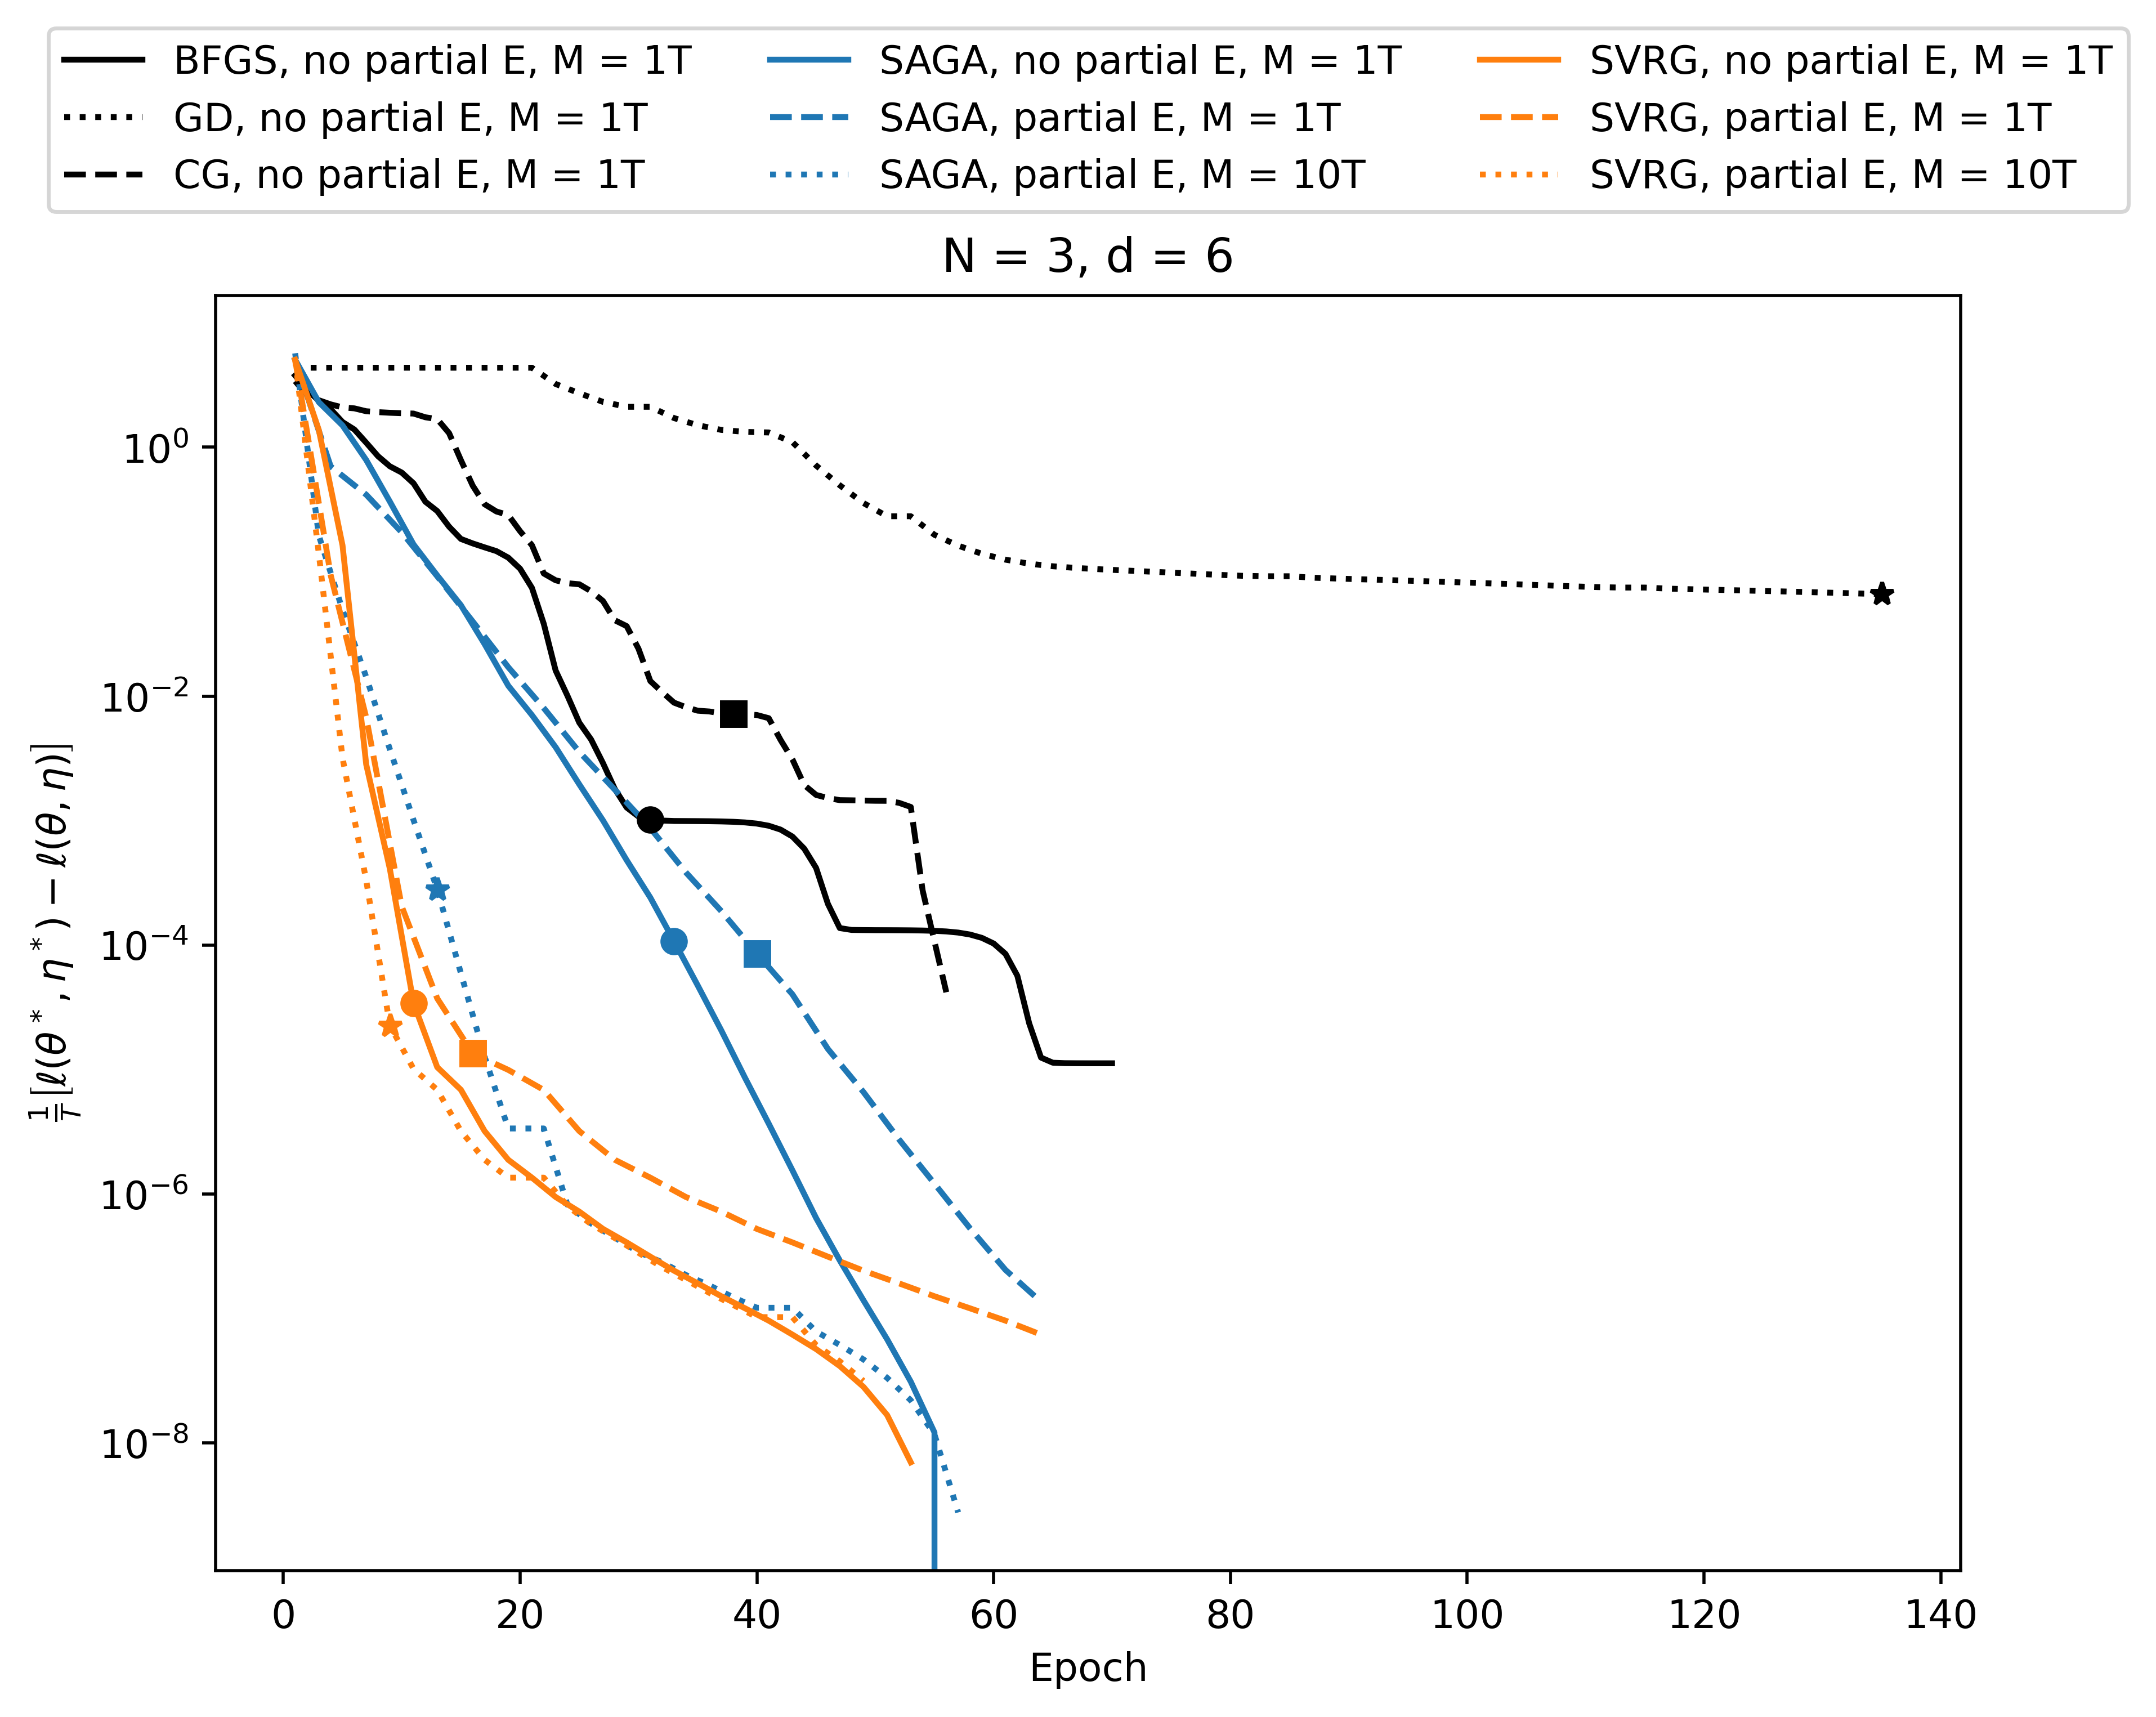
\includegraphics[width=3in]{../plt/log-like_v_epoch_T-100000-K-3-1-d-6-002.png}
    \\
    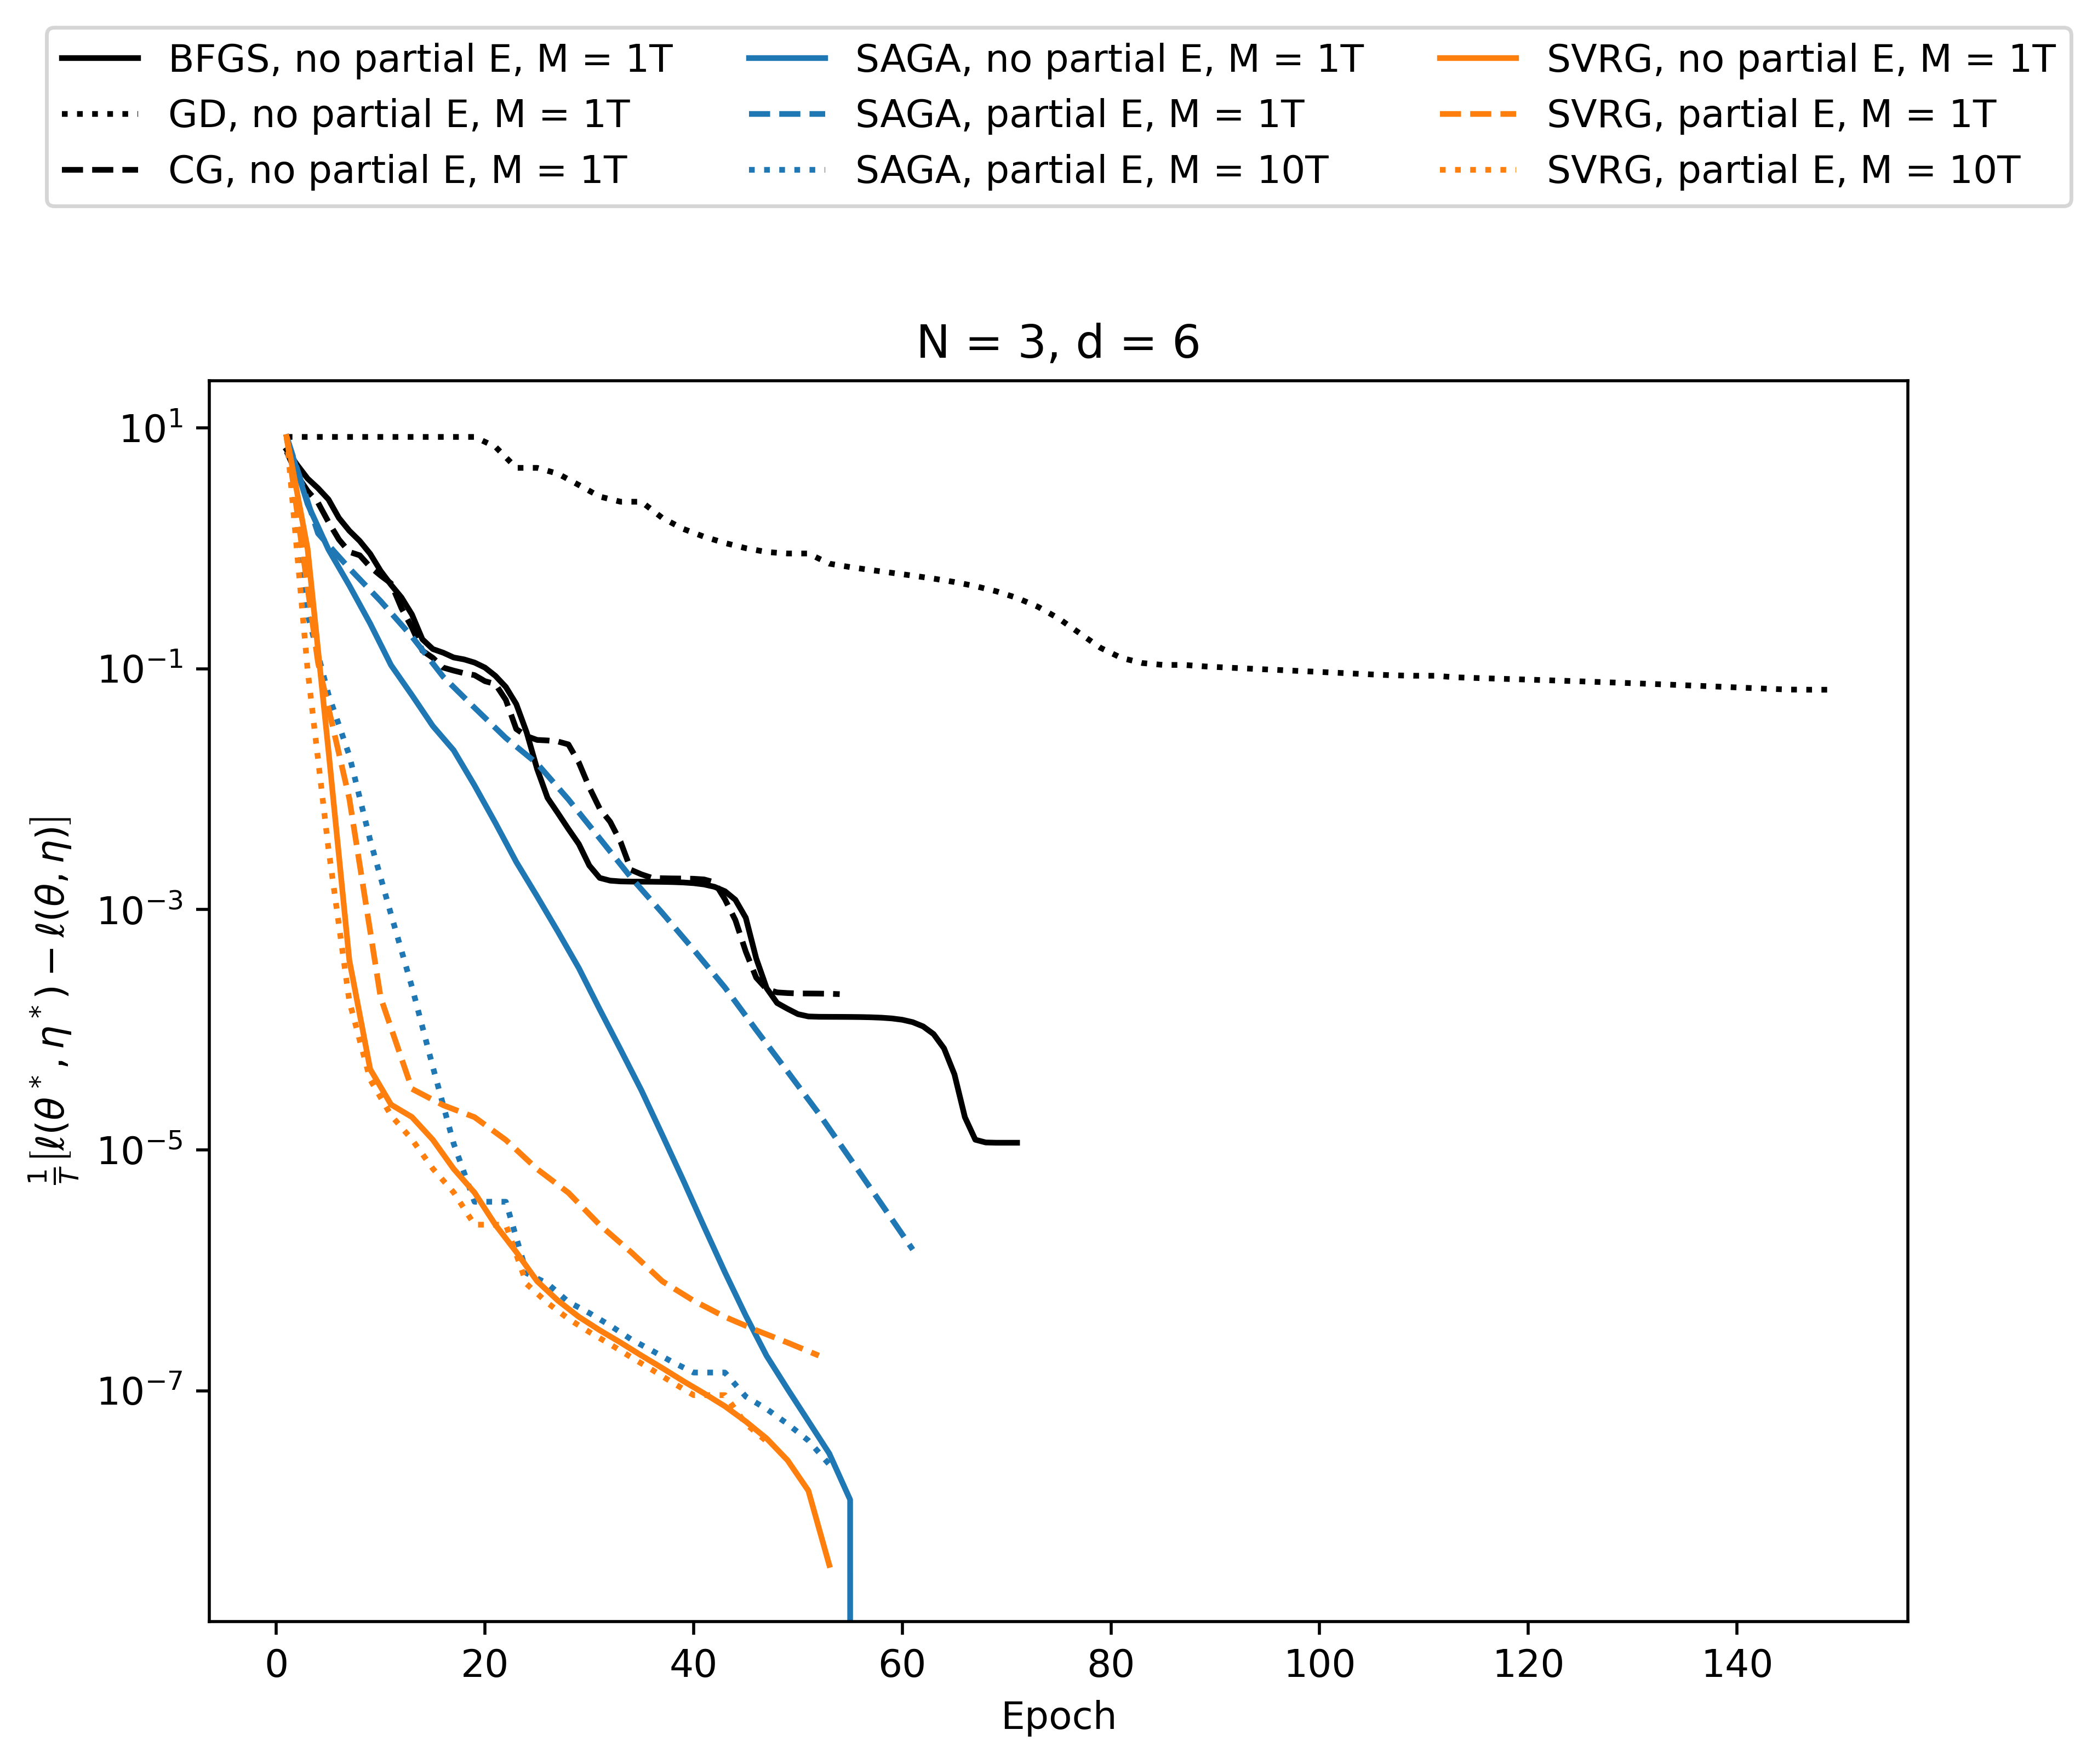
\includegraphics[width=3in]{../plt/log-like_v_epoch_T-100000-K-3-1-d-6-003.png}
    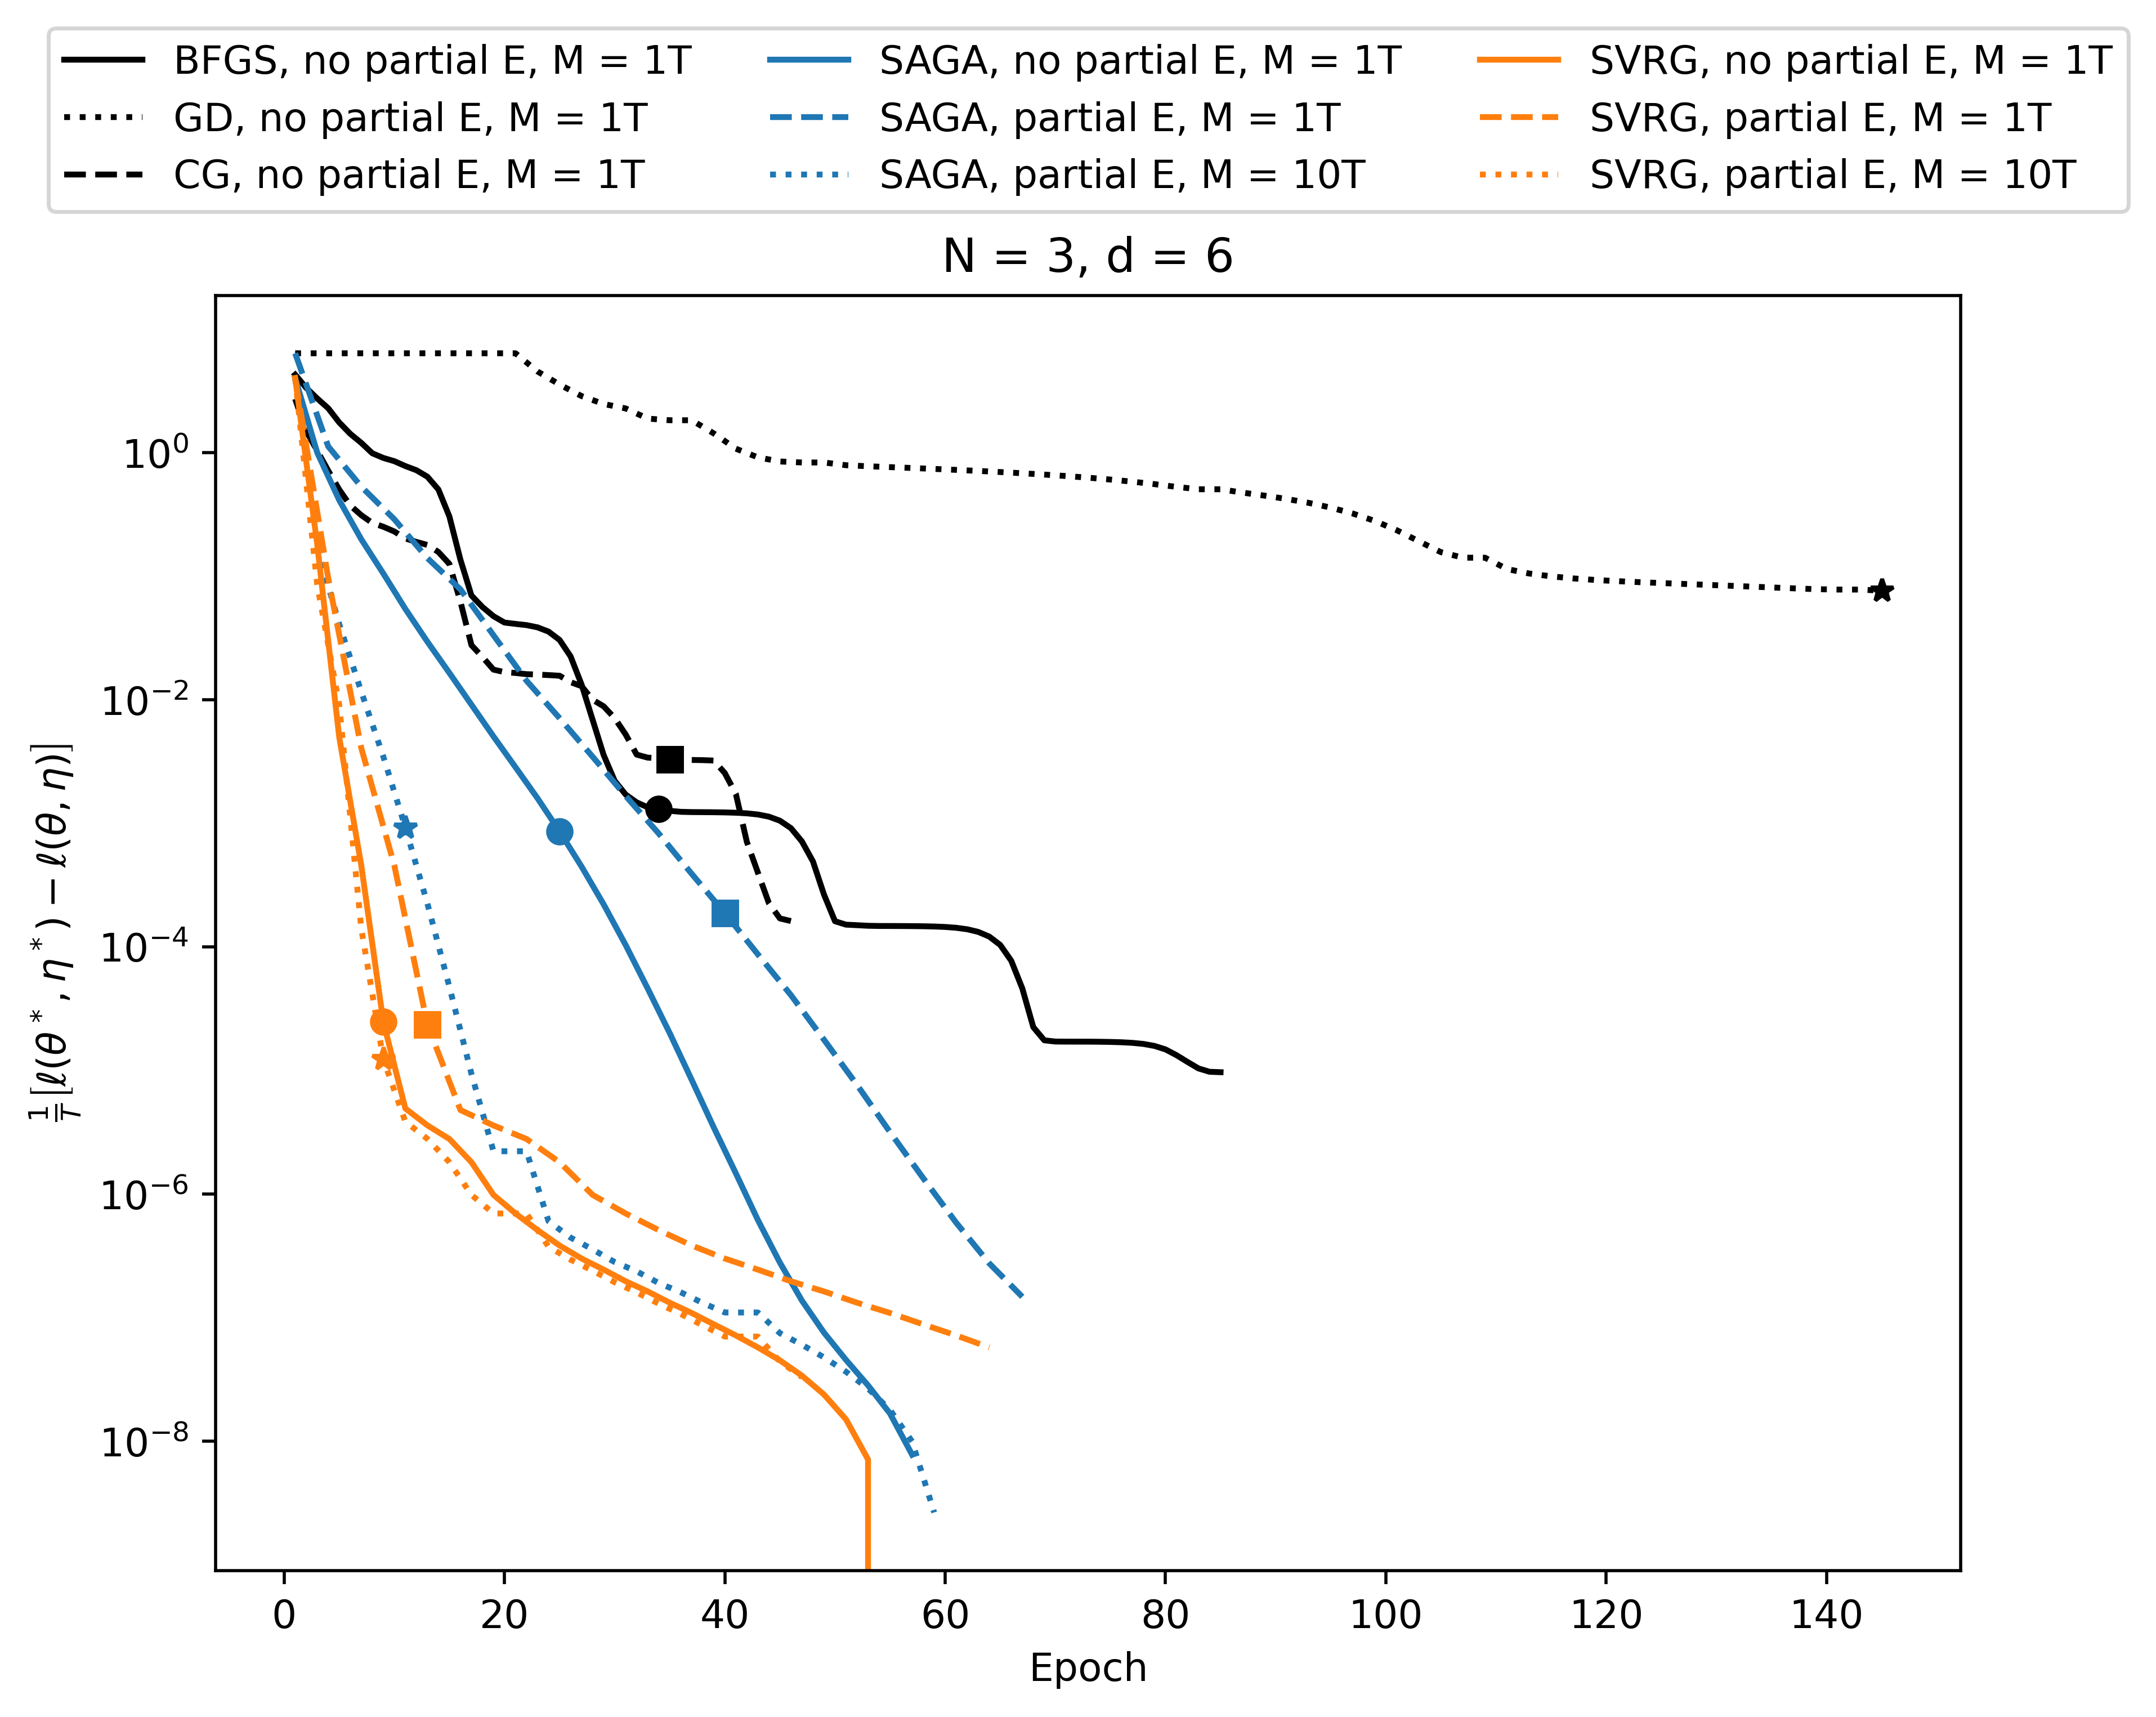
\includegraphics[width=3in]{../plt/log-like_v_epoch_T-100000-K-3-1-d-6-004.png}   
    \caption{Optimally gap between the current log-likelihood and optimal log-likelihood for the simulation studies with $T=10^{5}$, $N=3$ and $d=6$, for four different simulated data sets. One epoch represents either one full E-step, $T$ iterations with the M-step, or one gradient step for full-gradient algorithms. The y-axis is on a log-scale.}
\end{figure}
%
\begin{figure}
    \centering
    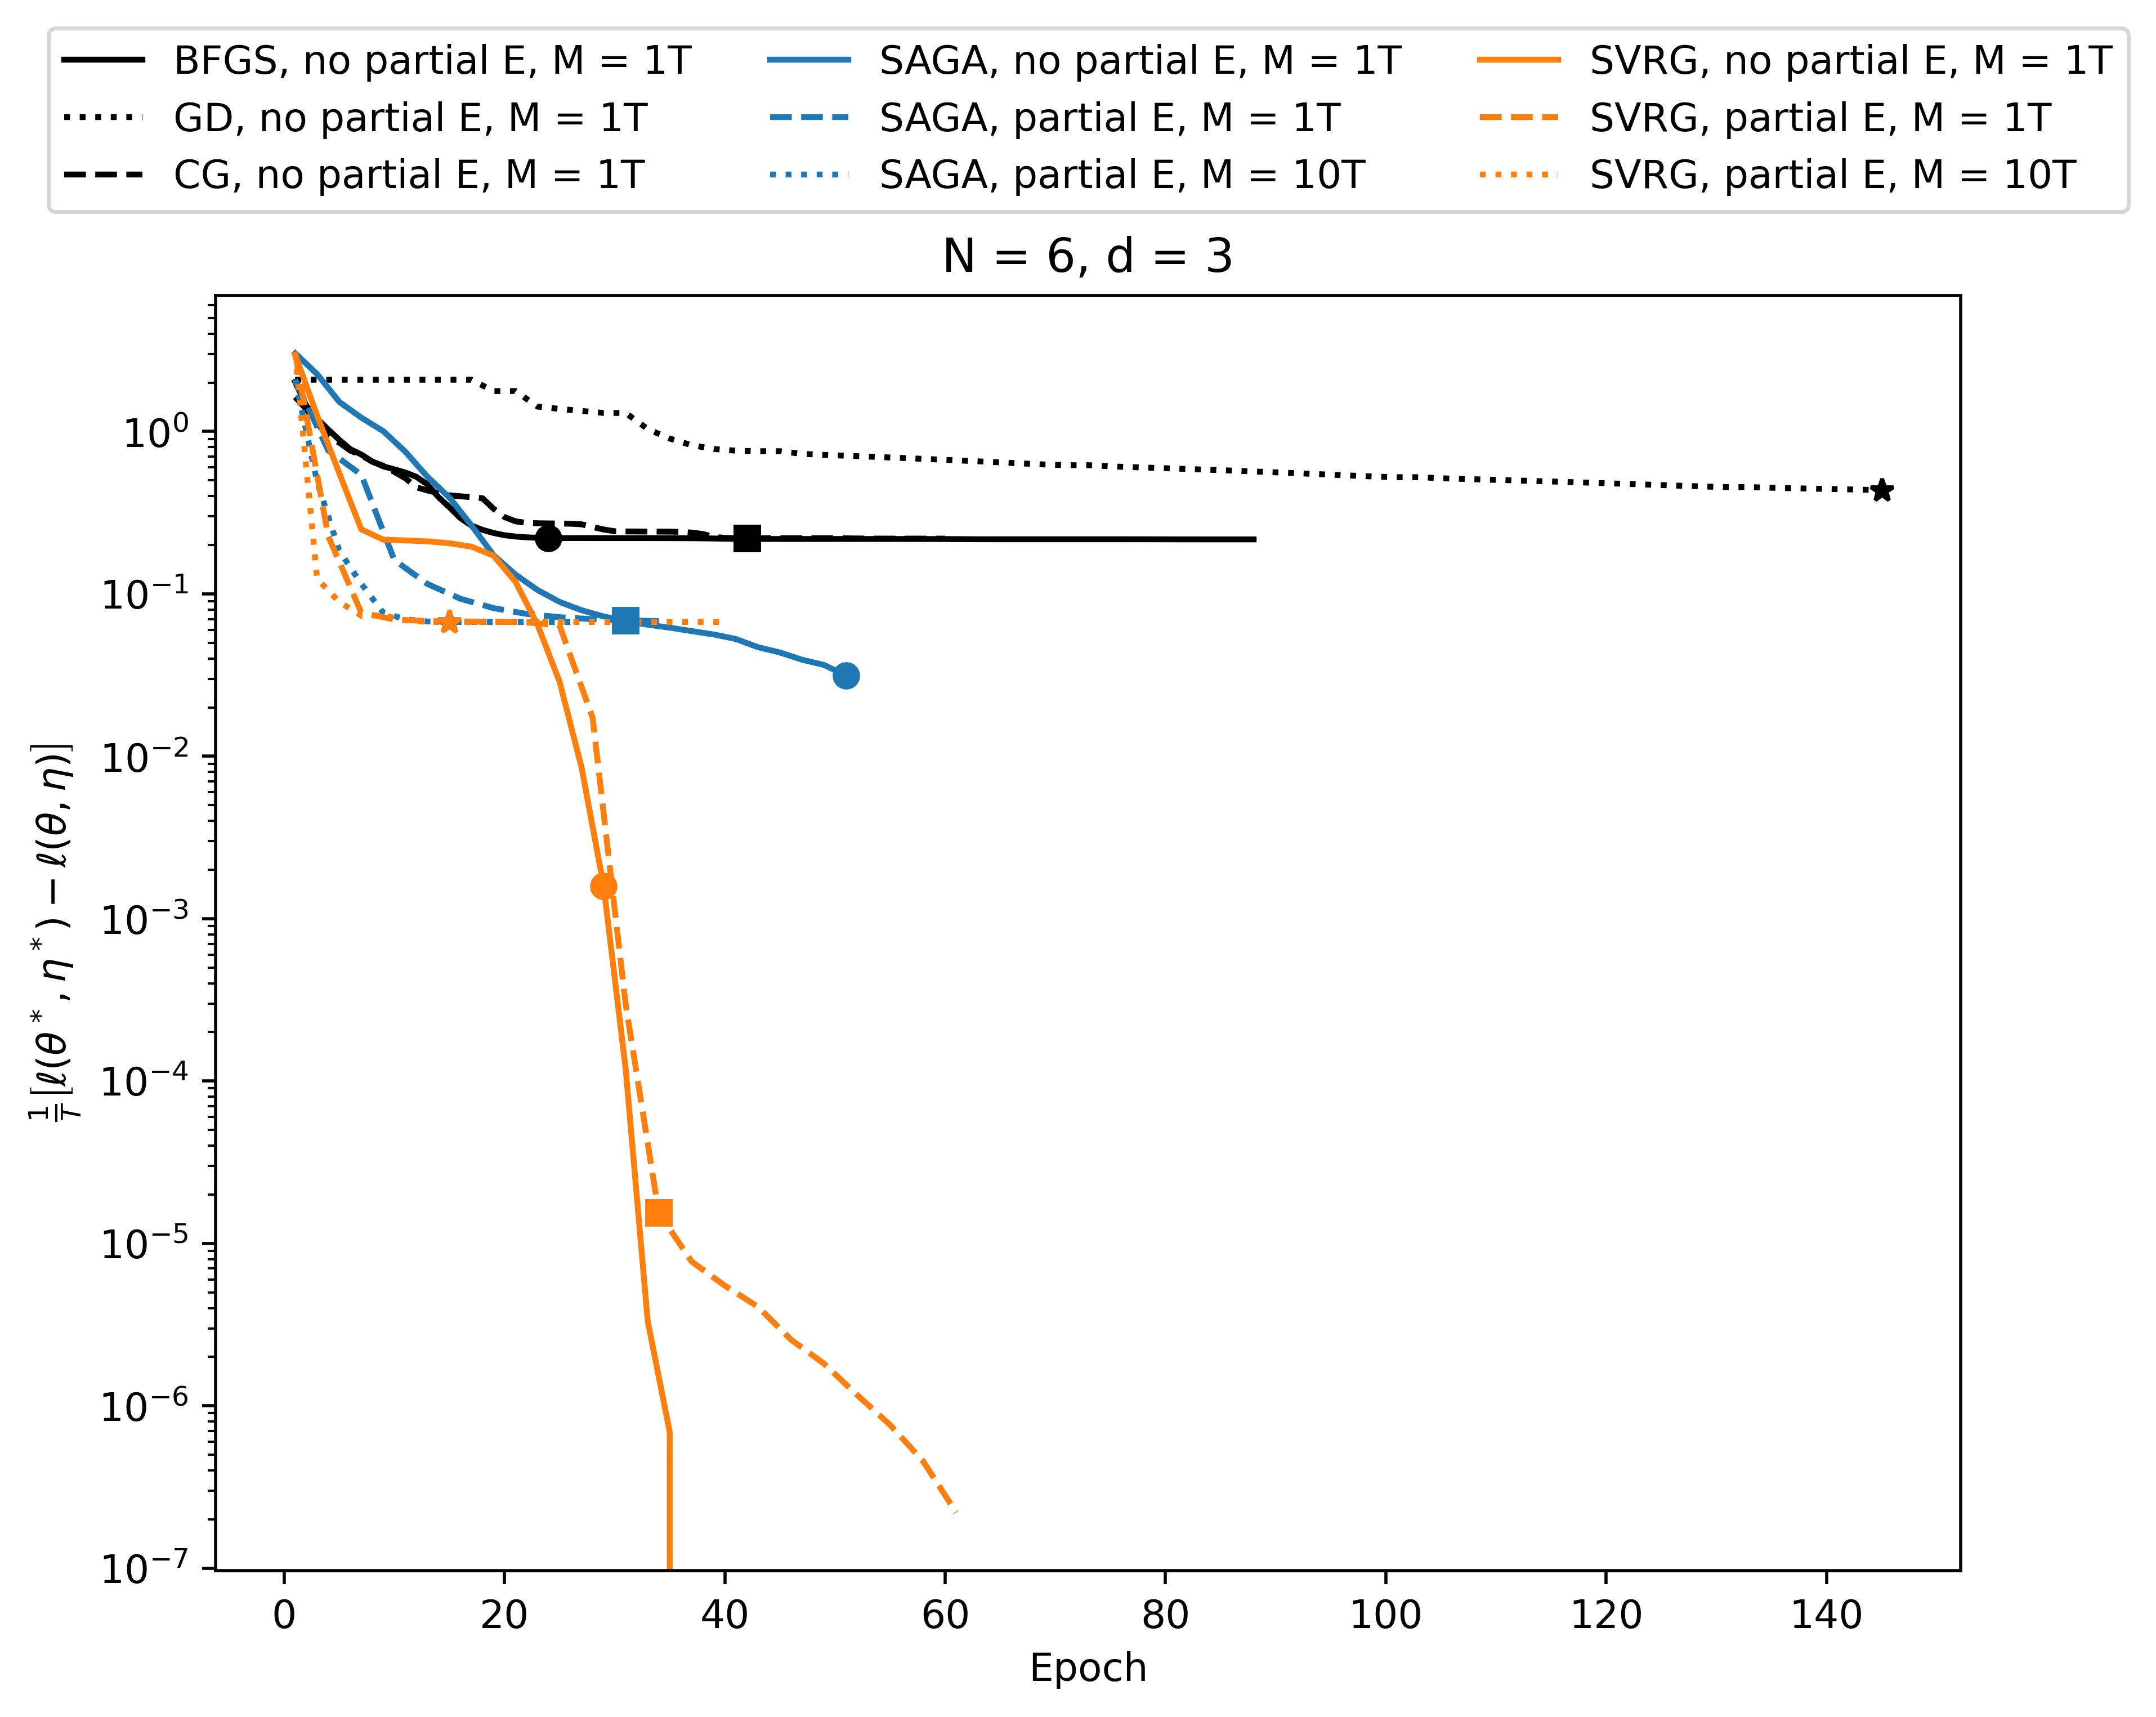
\includegraphics[width=3in]{../plt/log-like_v_epoch_T-100000-K-6-1-d-3-001.png}
    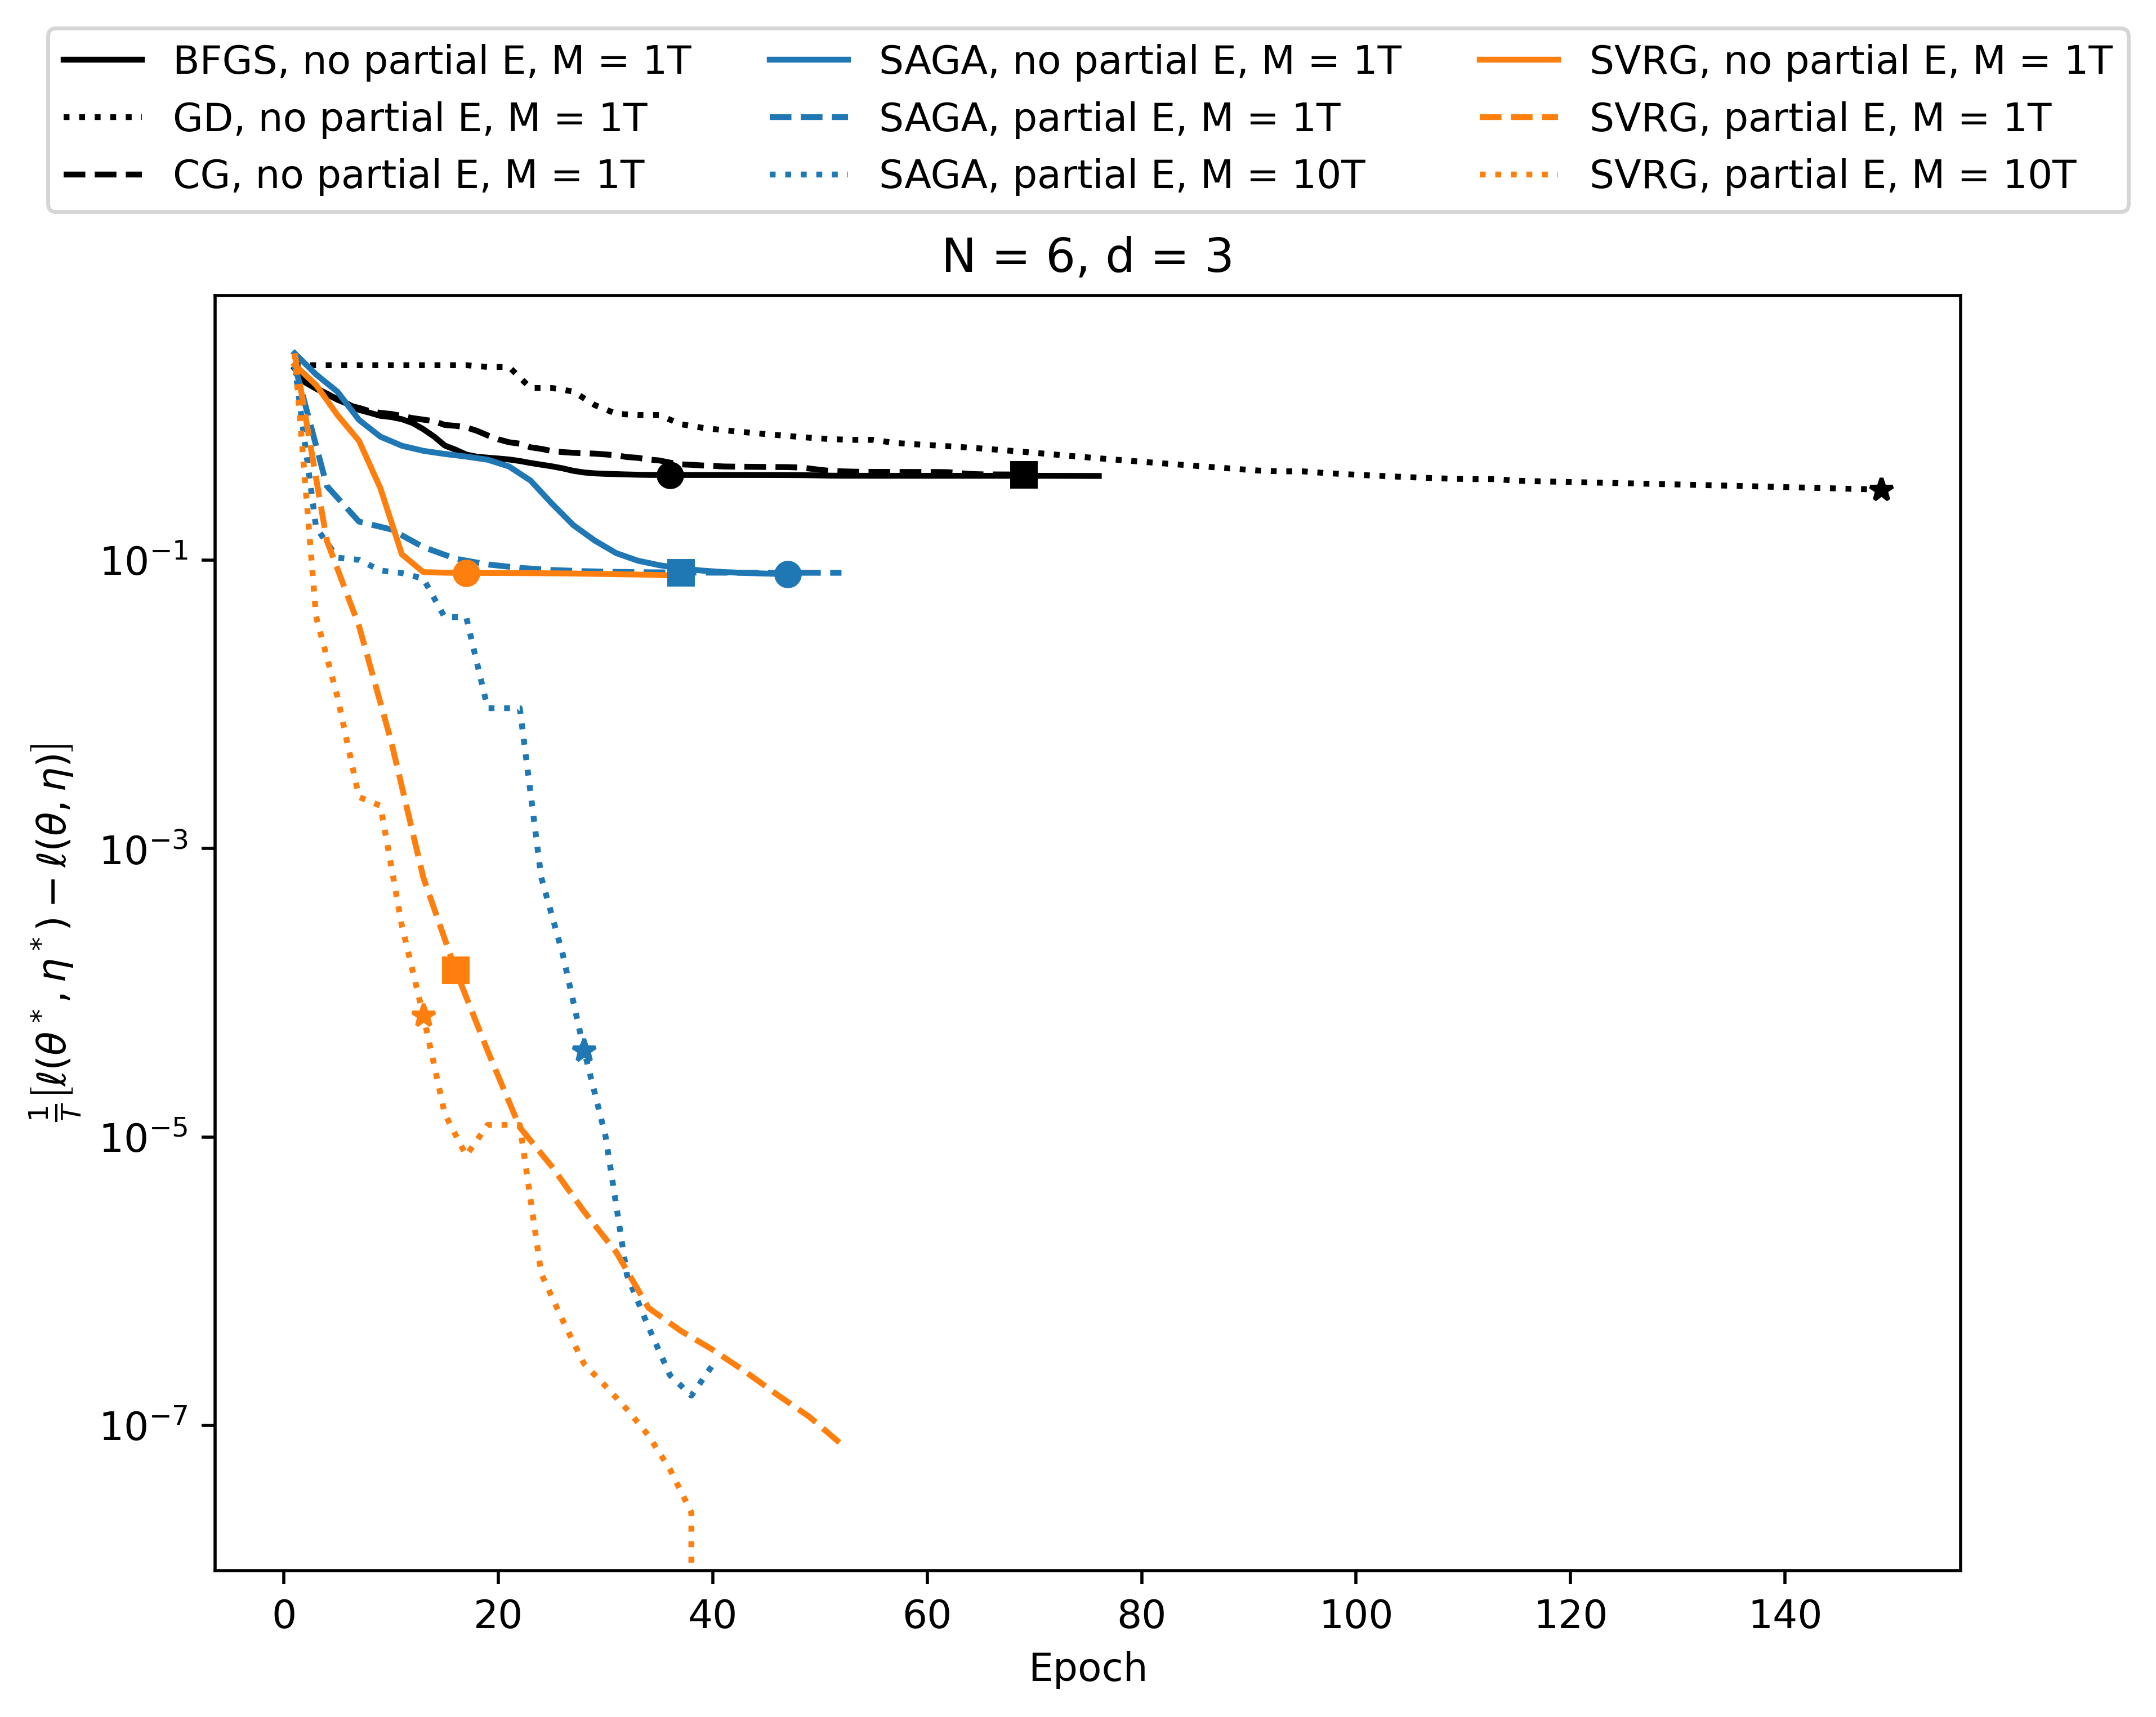
\includegraphics[width=3in]{../plt/log-like_v_epoch_T-100000-K-6-1-d-3-002.png}
    \\
    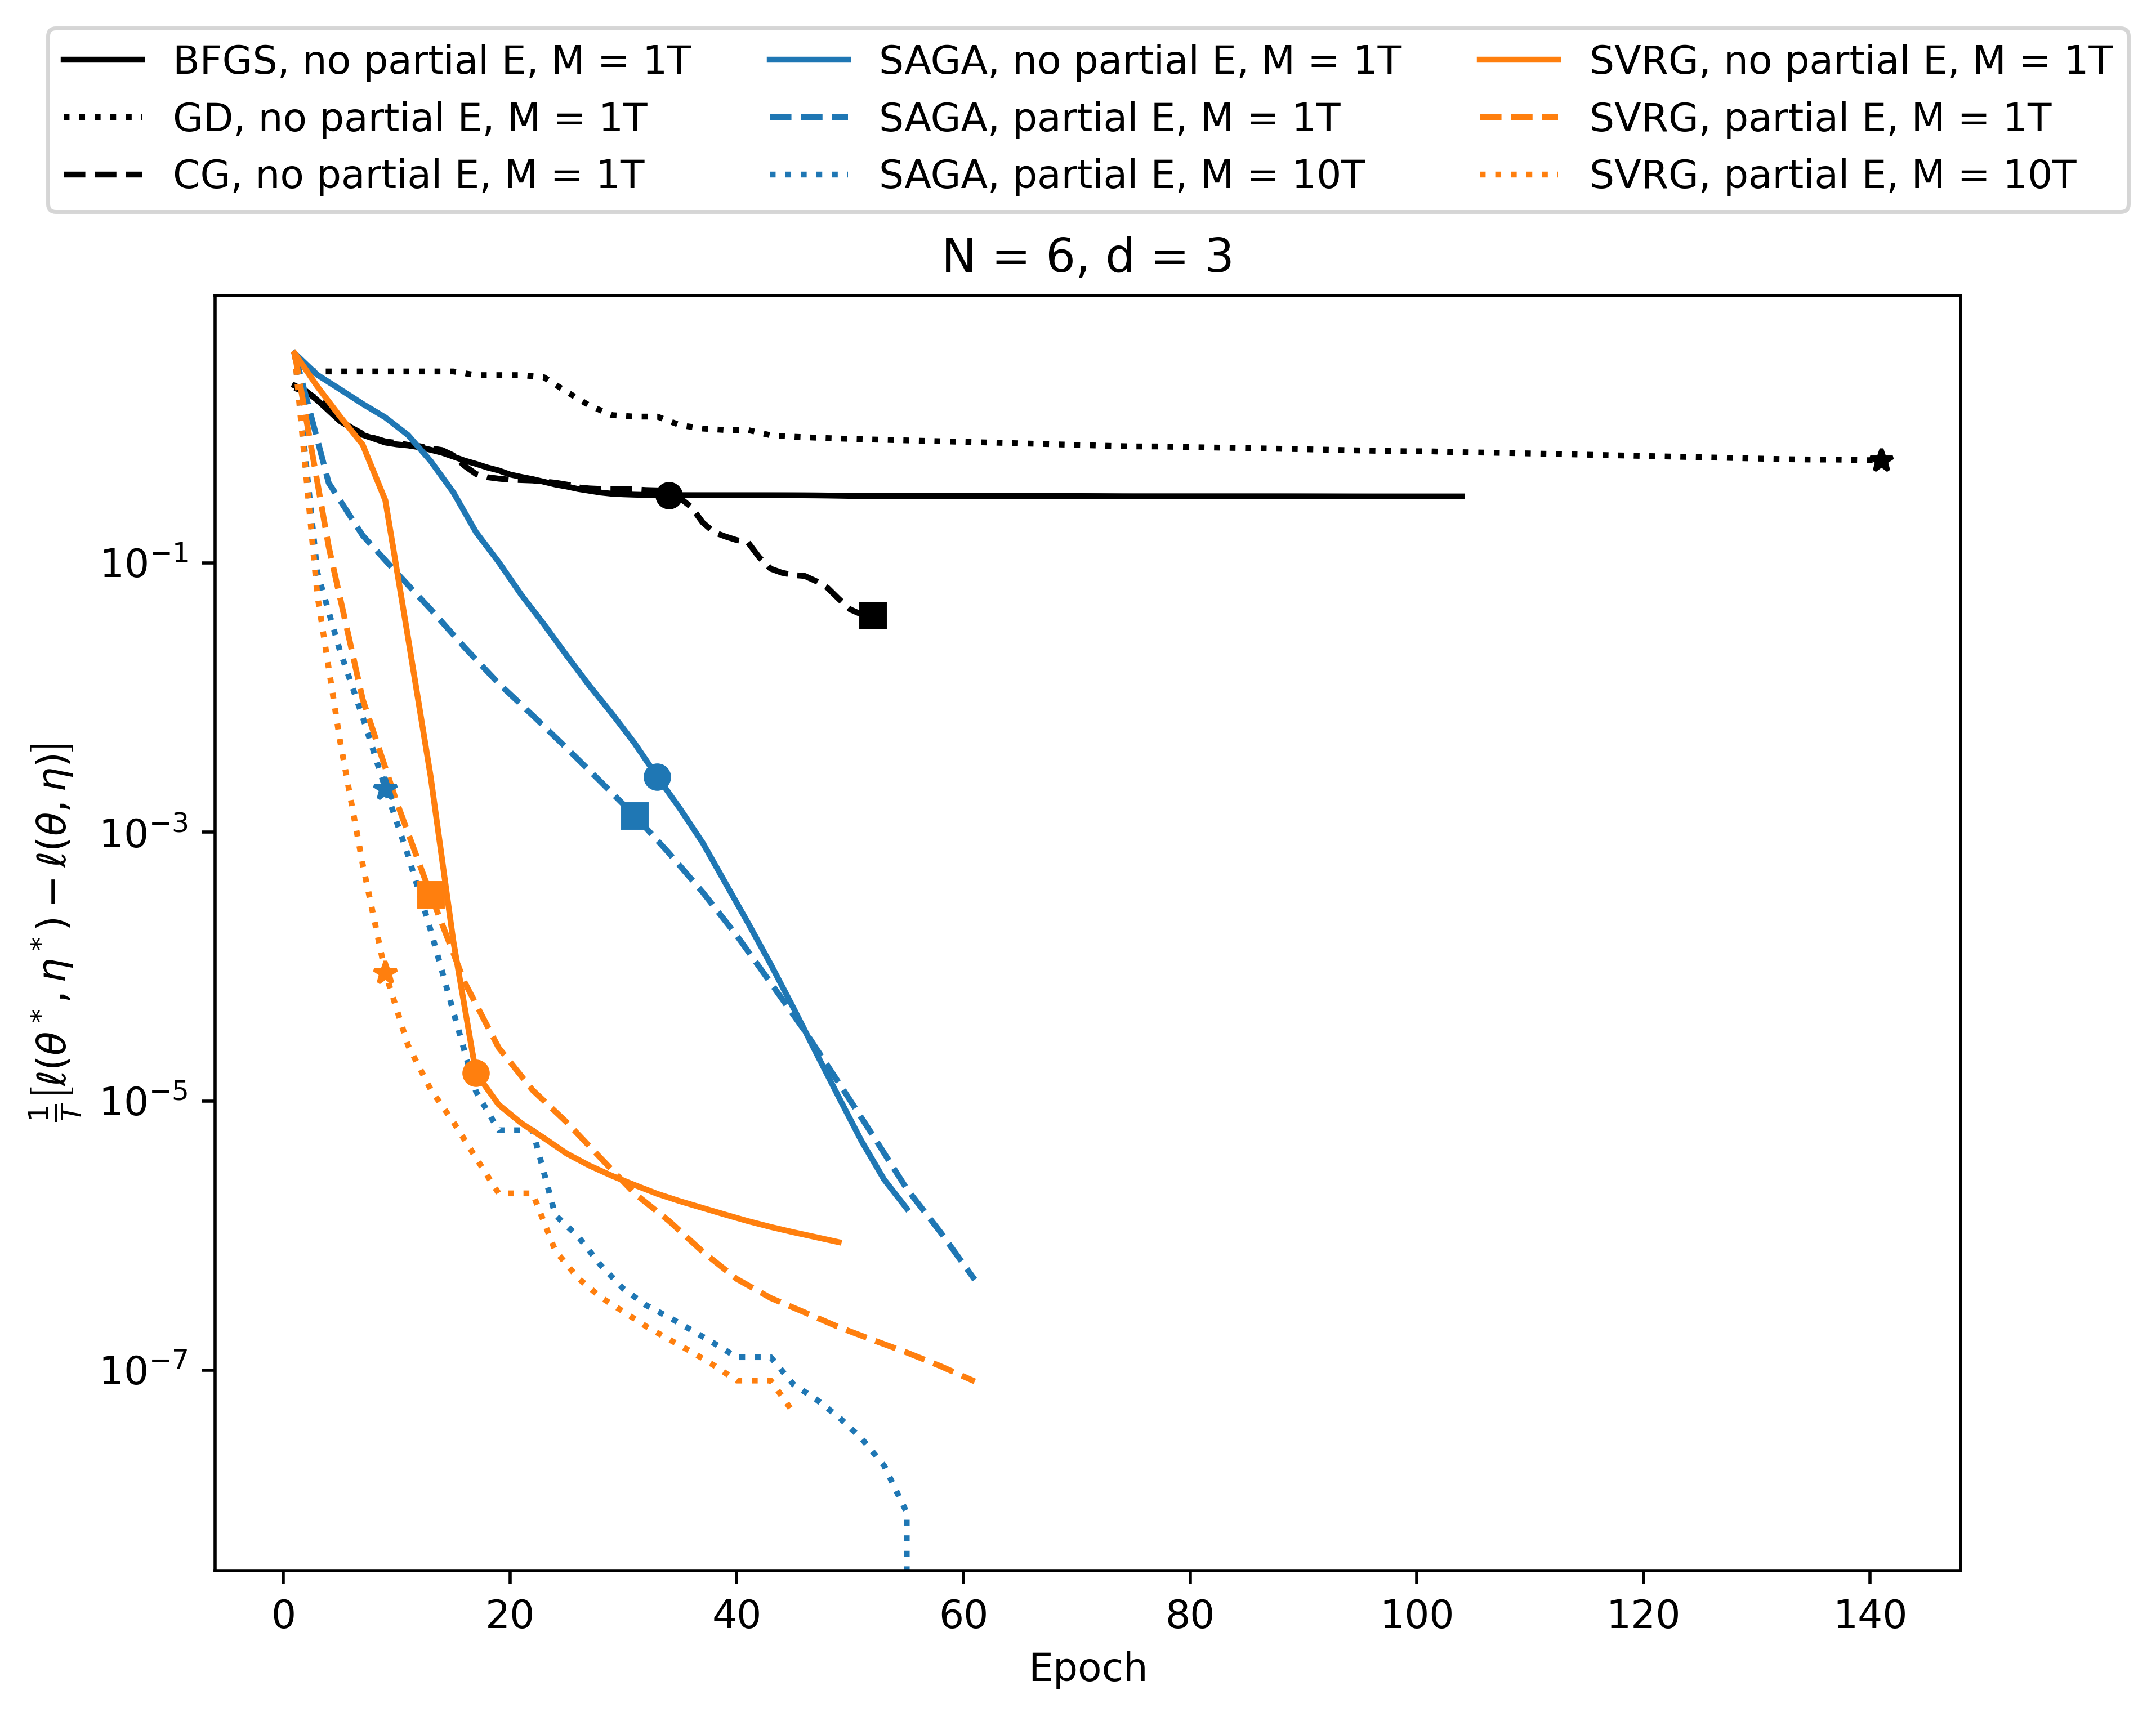
\includegraphics[width=3in]{../plt/log-like_v_epoch_T-100000-K-6-1-d-3-003.png}
    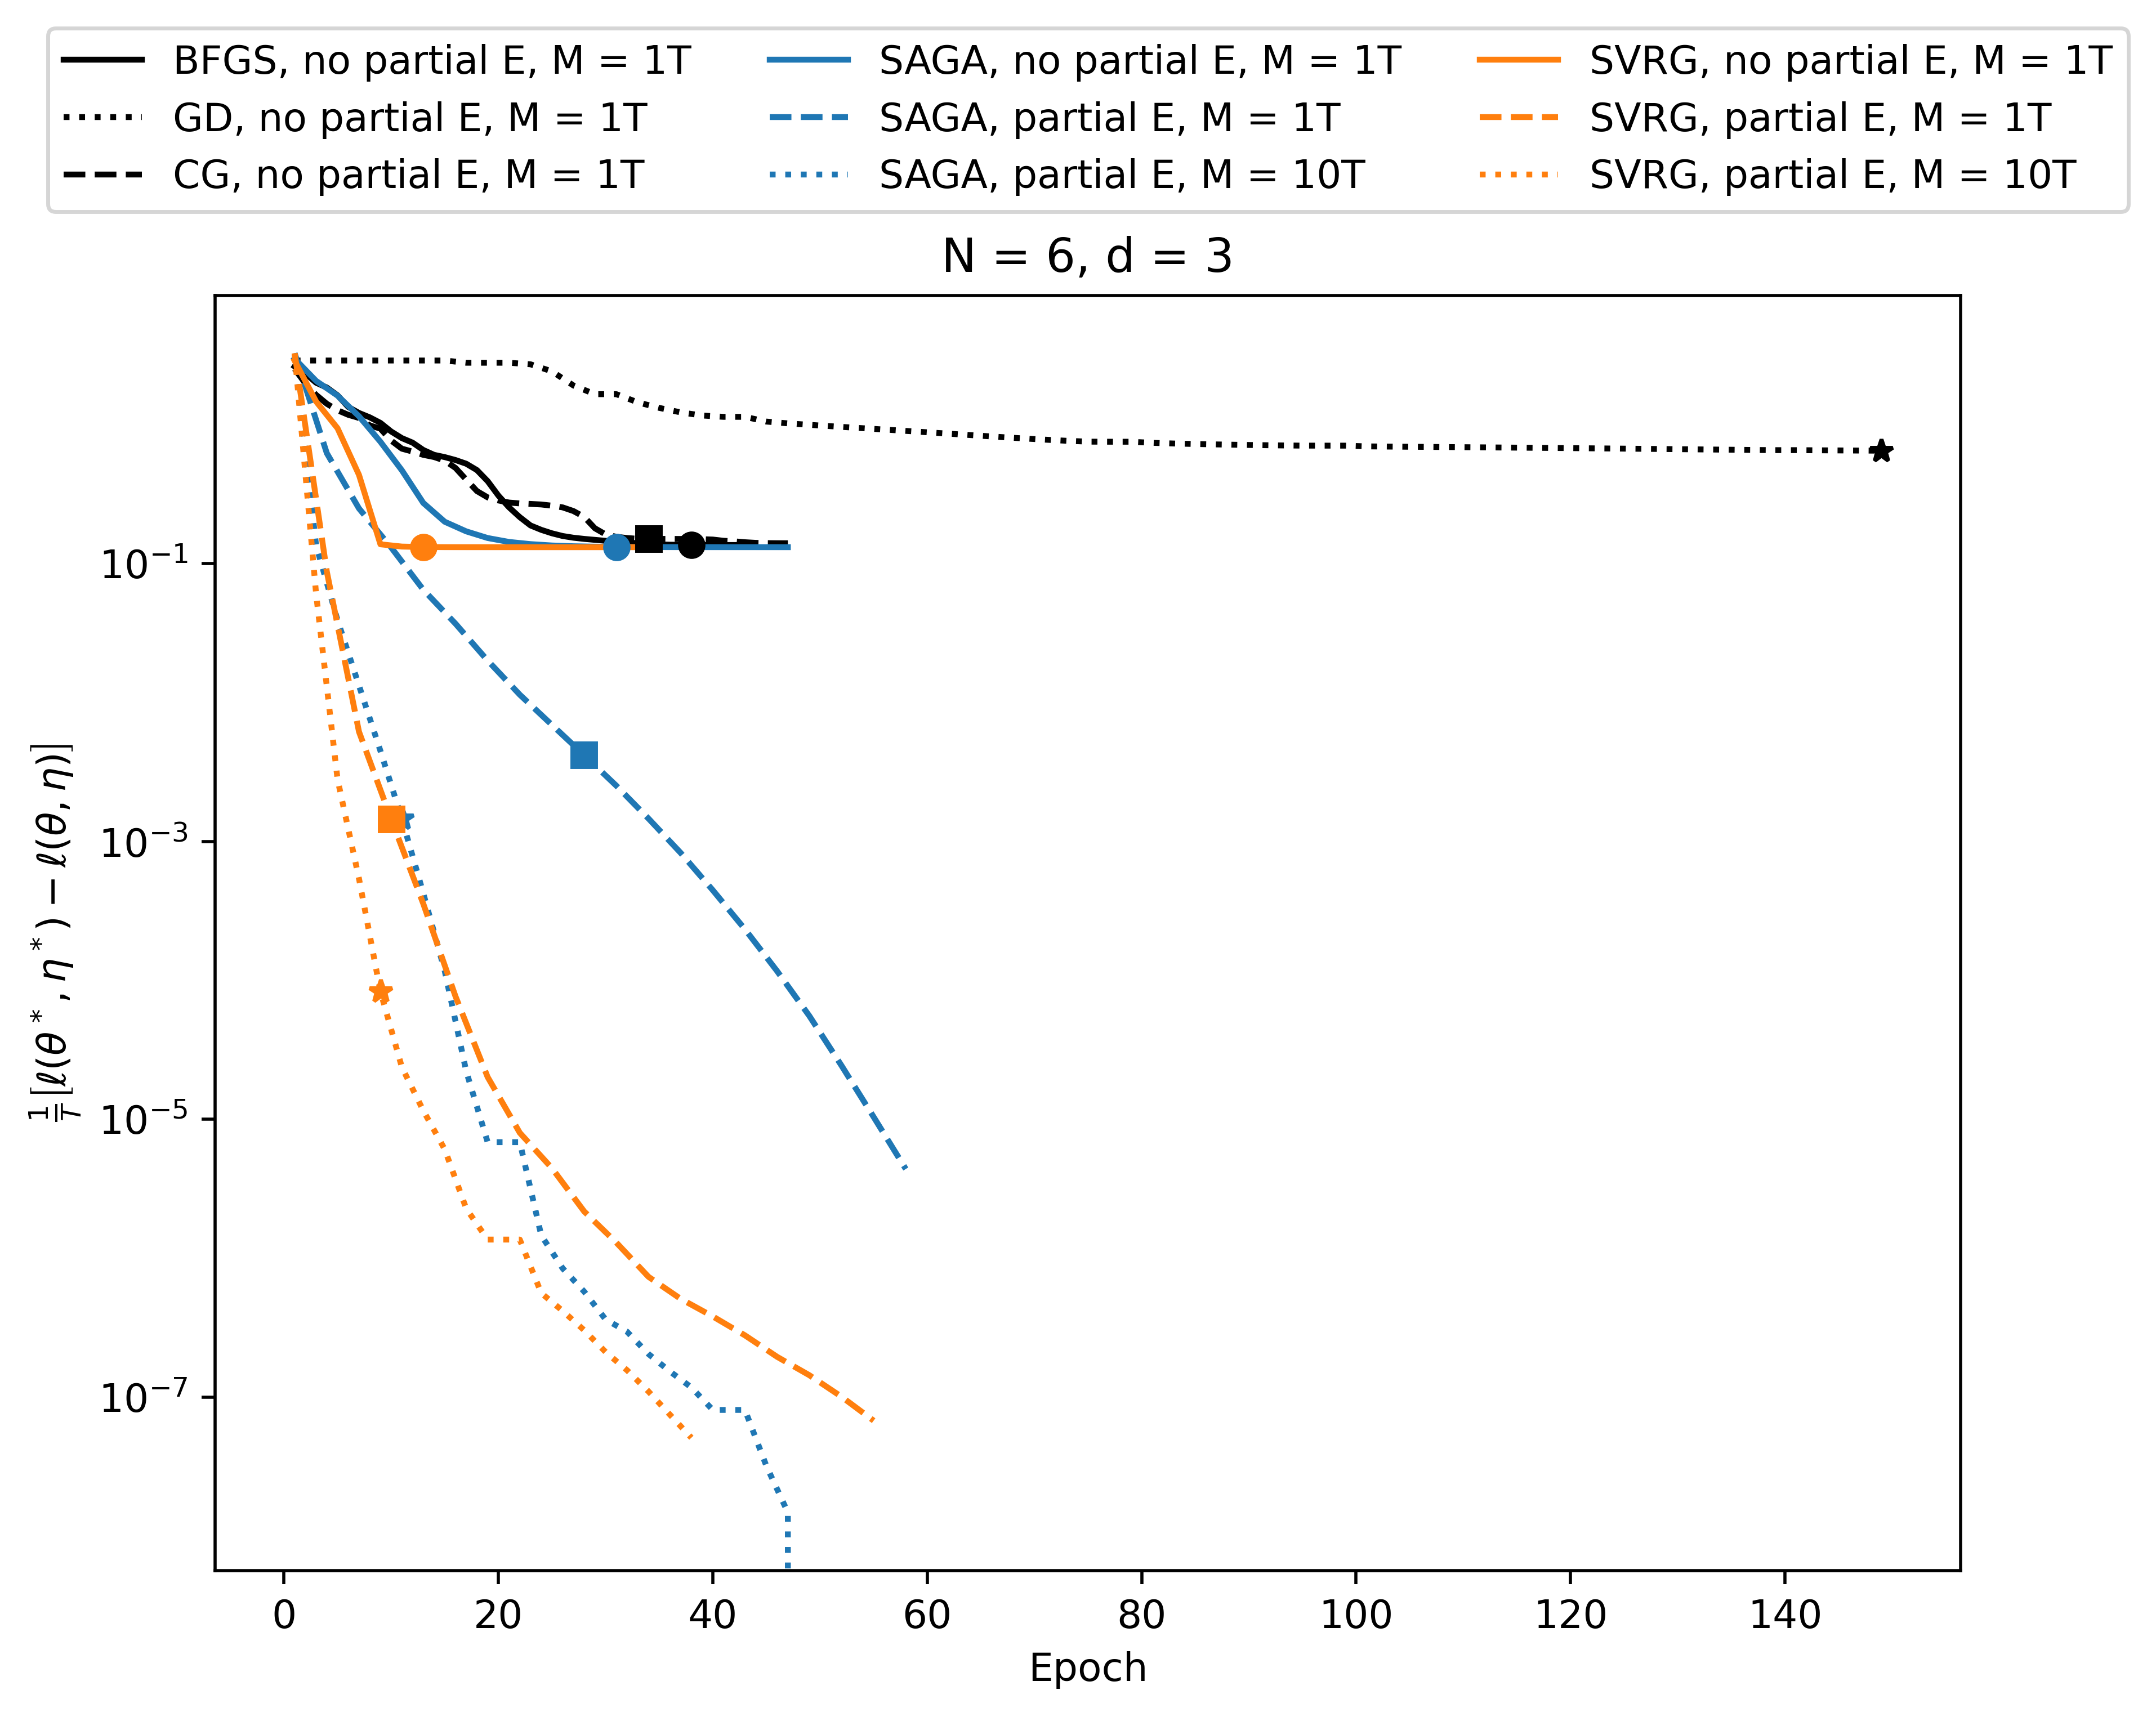
\includegraphics[width=3in]{../plt/log-like_v_epoch_T-100000-K-6-1-d-3-004.png}   
    \caption{Optimally gap between the current log-likelihood and optimal log-likelihood for the simulation studies with $T=10^{5}$, $N=6$ and $d=3$, for four different simulated data sets. One epoch represents either one full E-step, $T$ iterations with the M-step, or one gradient step for full-gradient algorithms. The y-axis is on a log-scale.}
\end{figure}
%
\begin{figure}
    \centering
    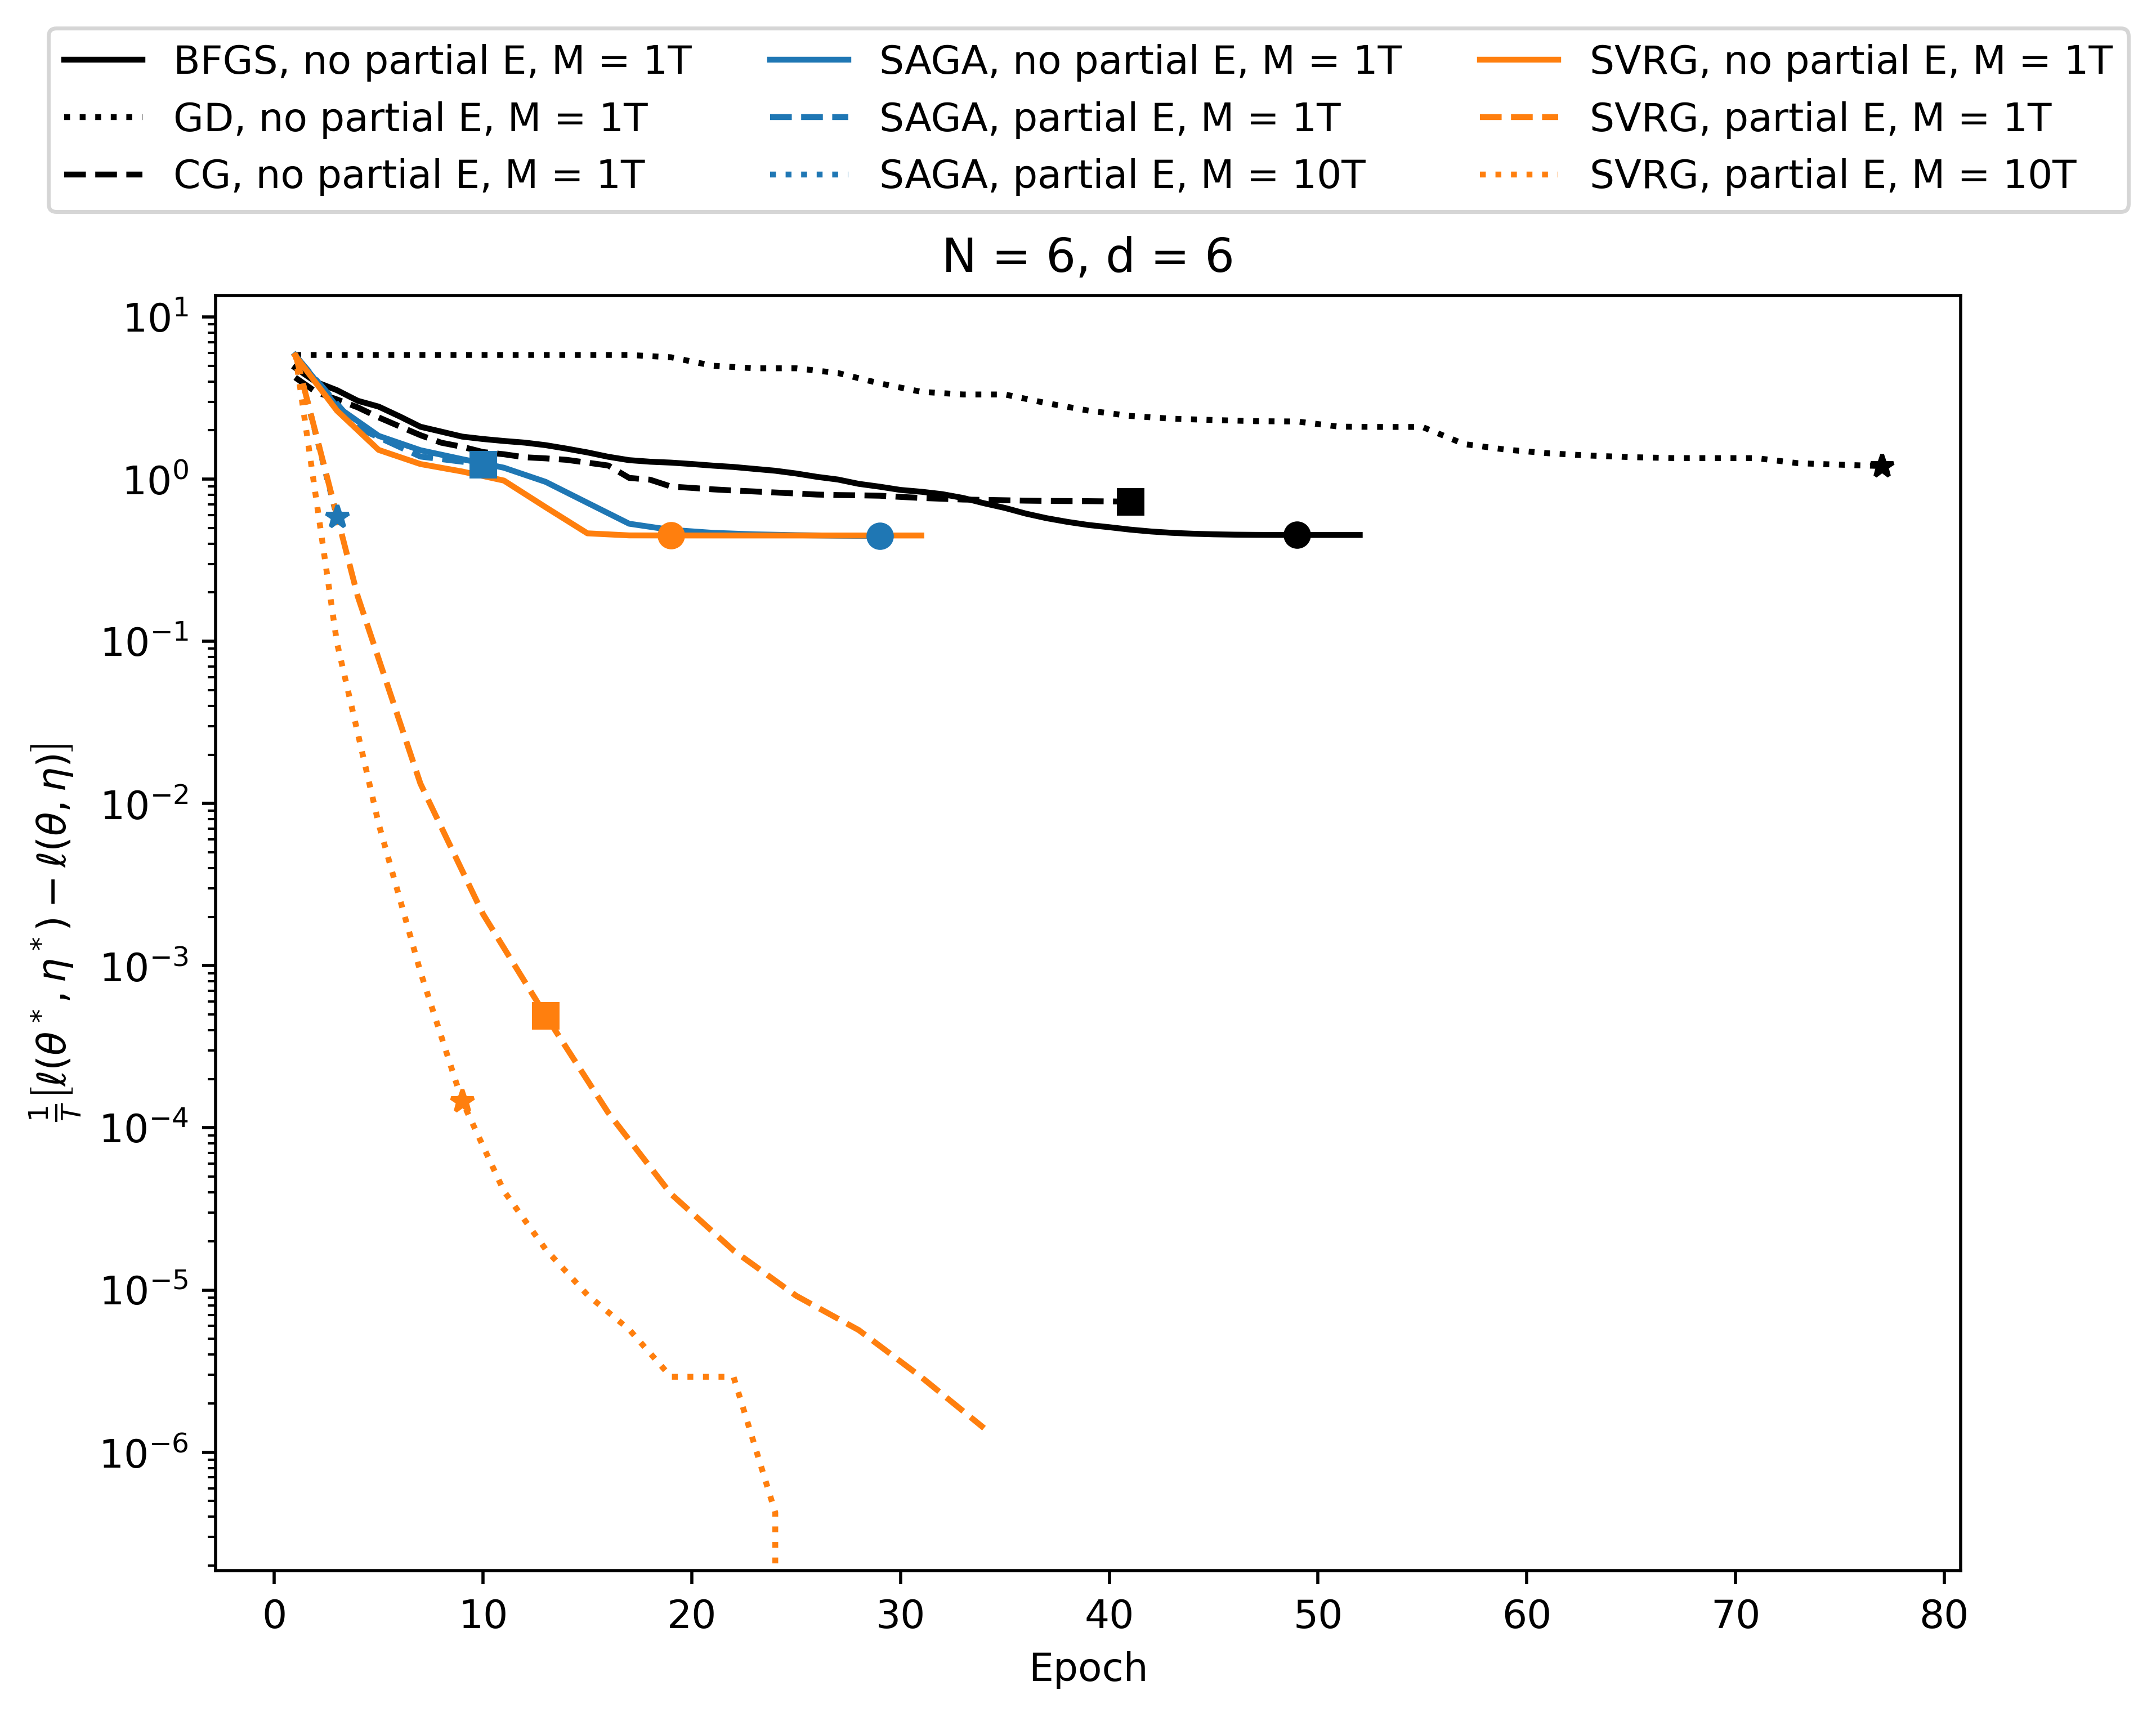
\includegraphics[width=3in]{../plt/log-like_v_epoch_T-100000-K-6-1-d-6-001.png}
    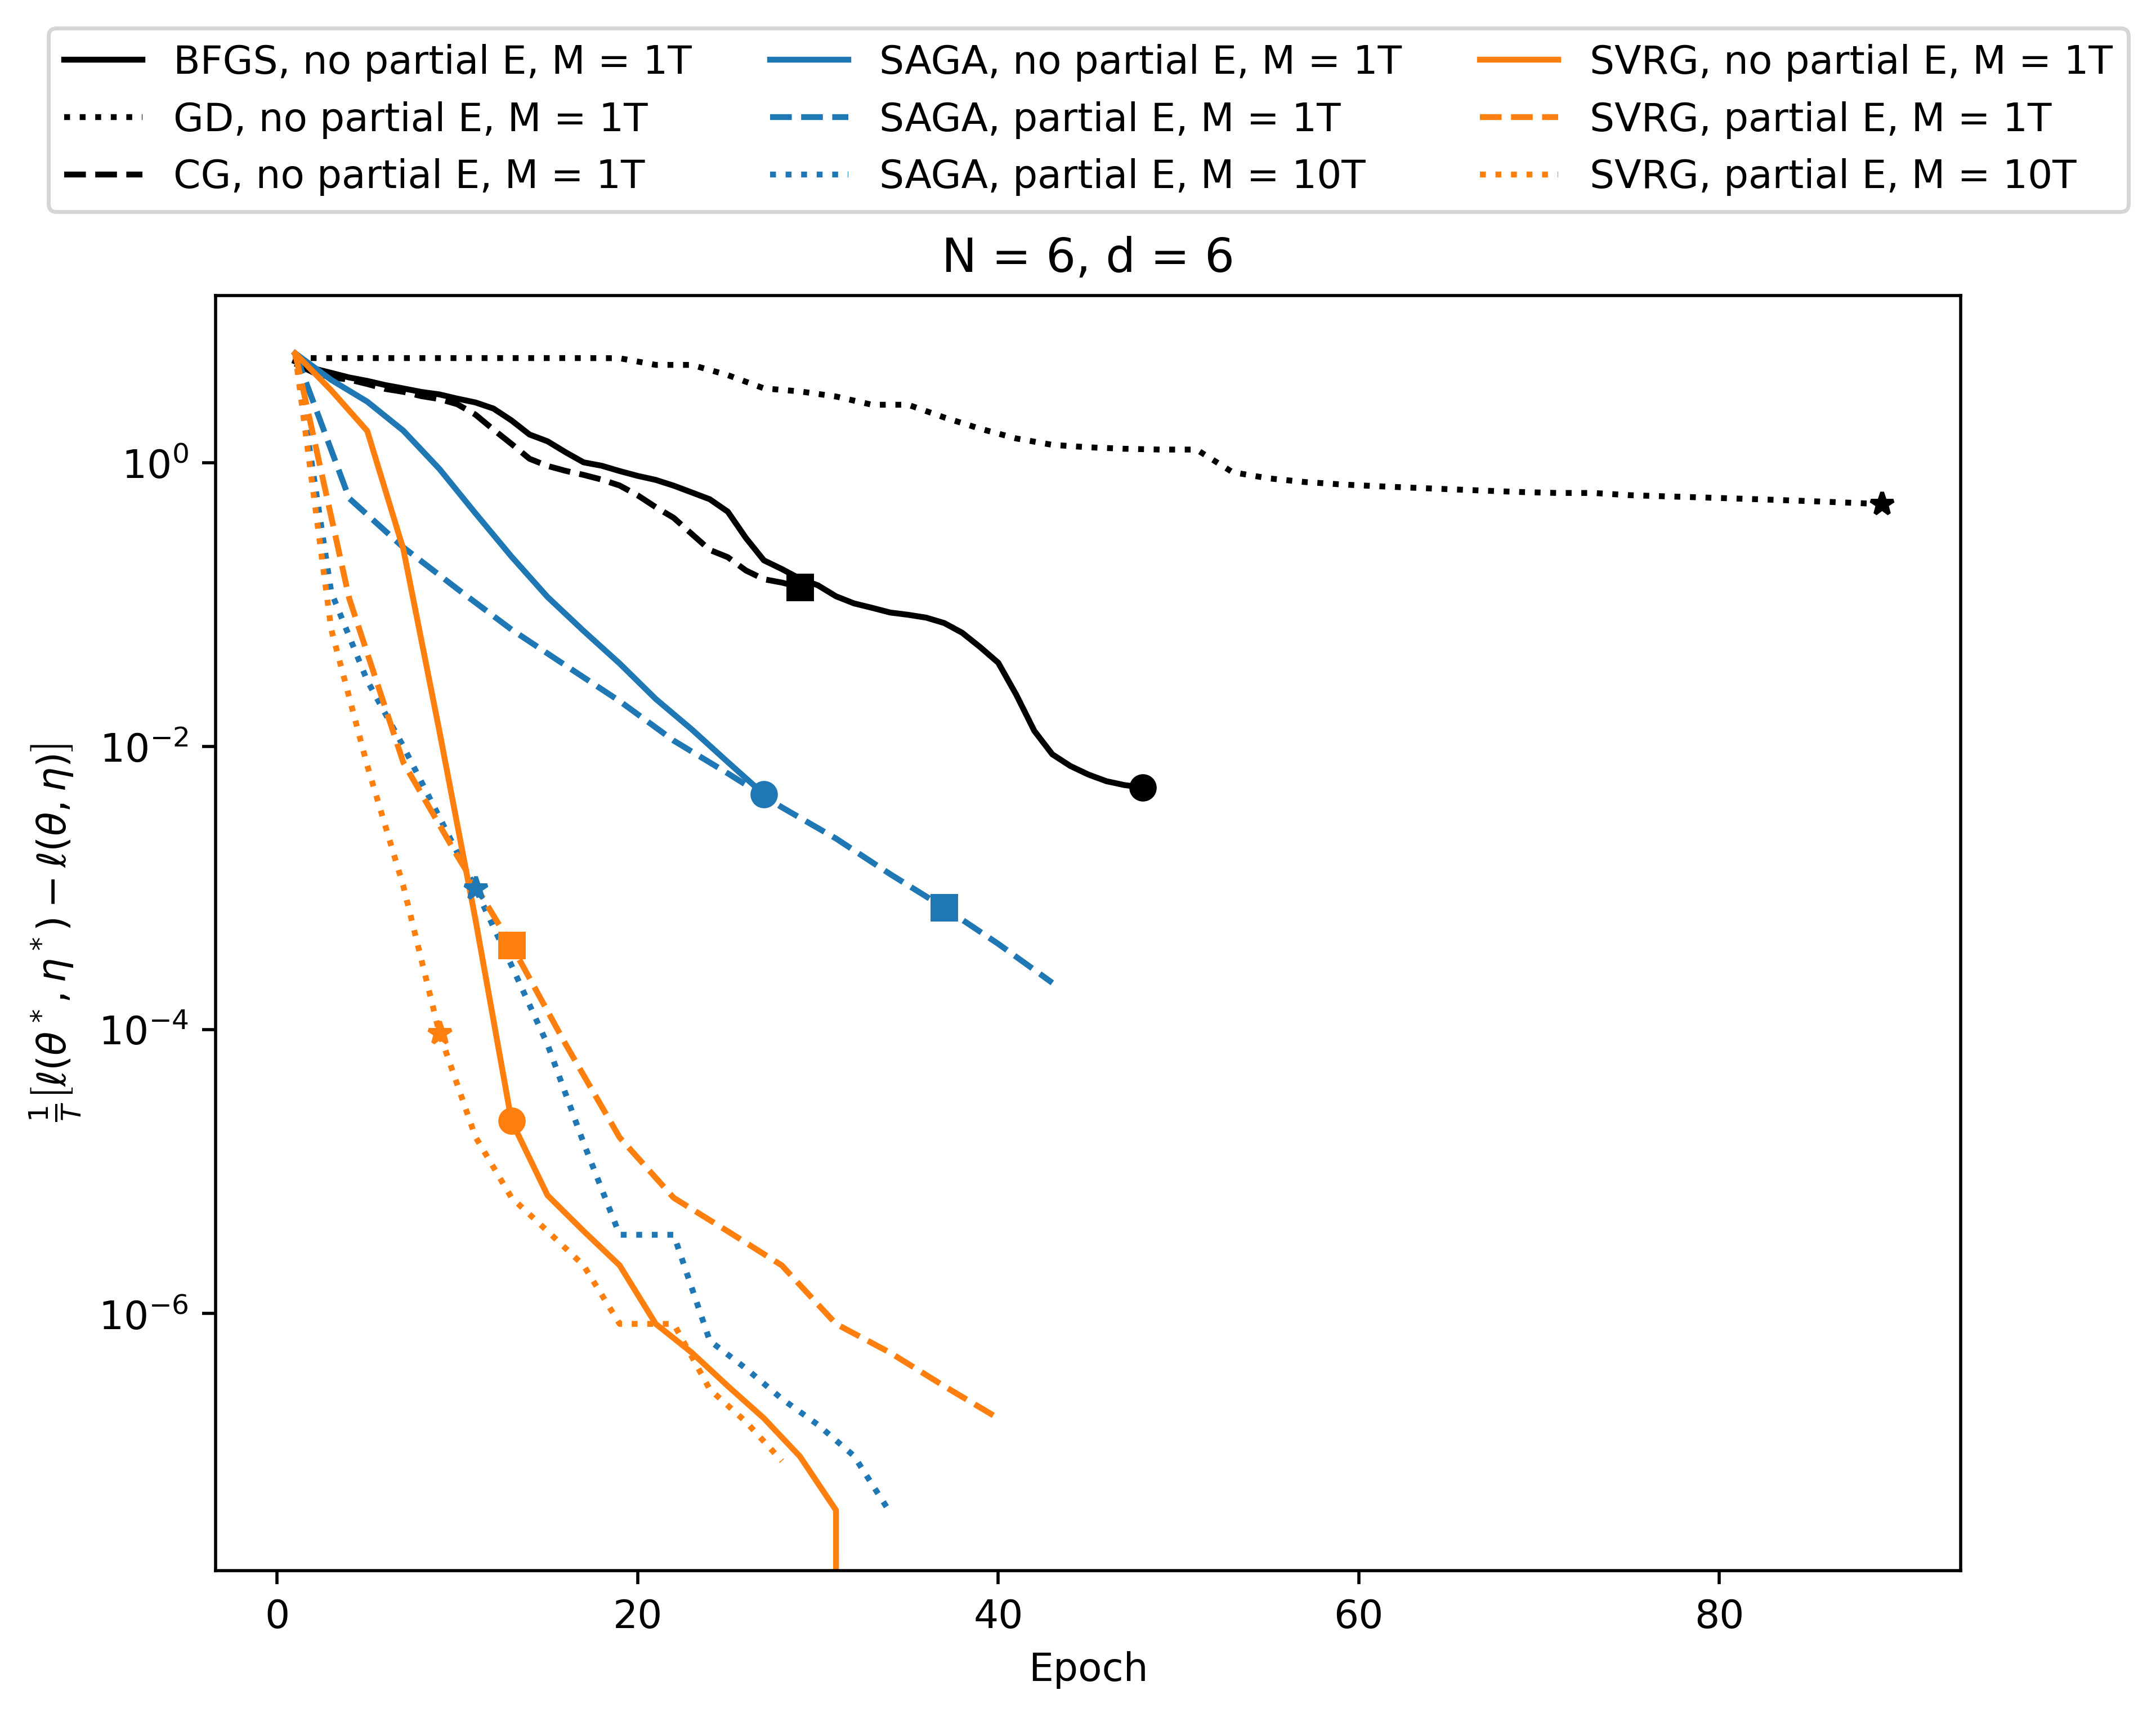
\includegraphics[width=3in]{../plt/log-like_v_epoch_T-100000-K-6-1-d-6-002.png}
    \\
    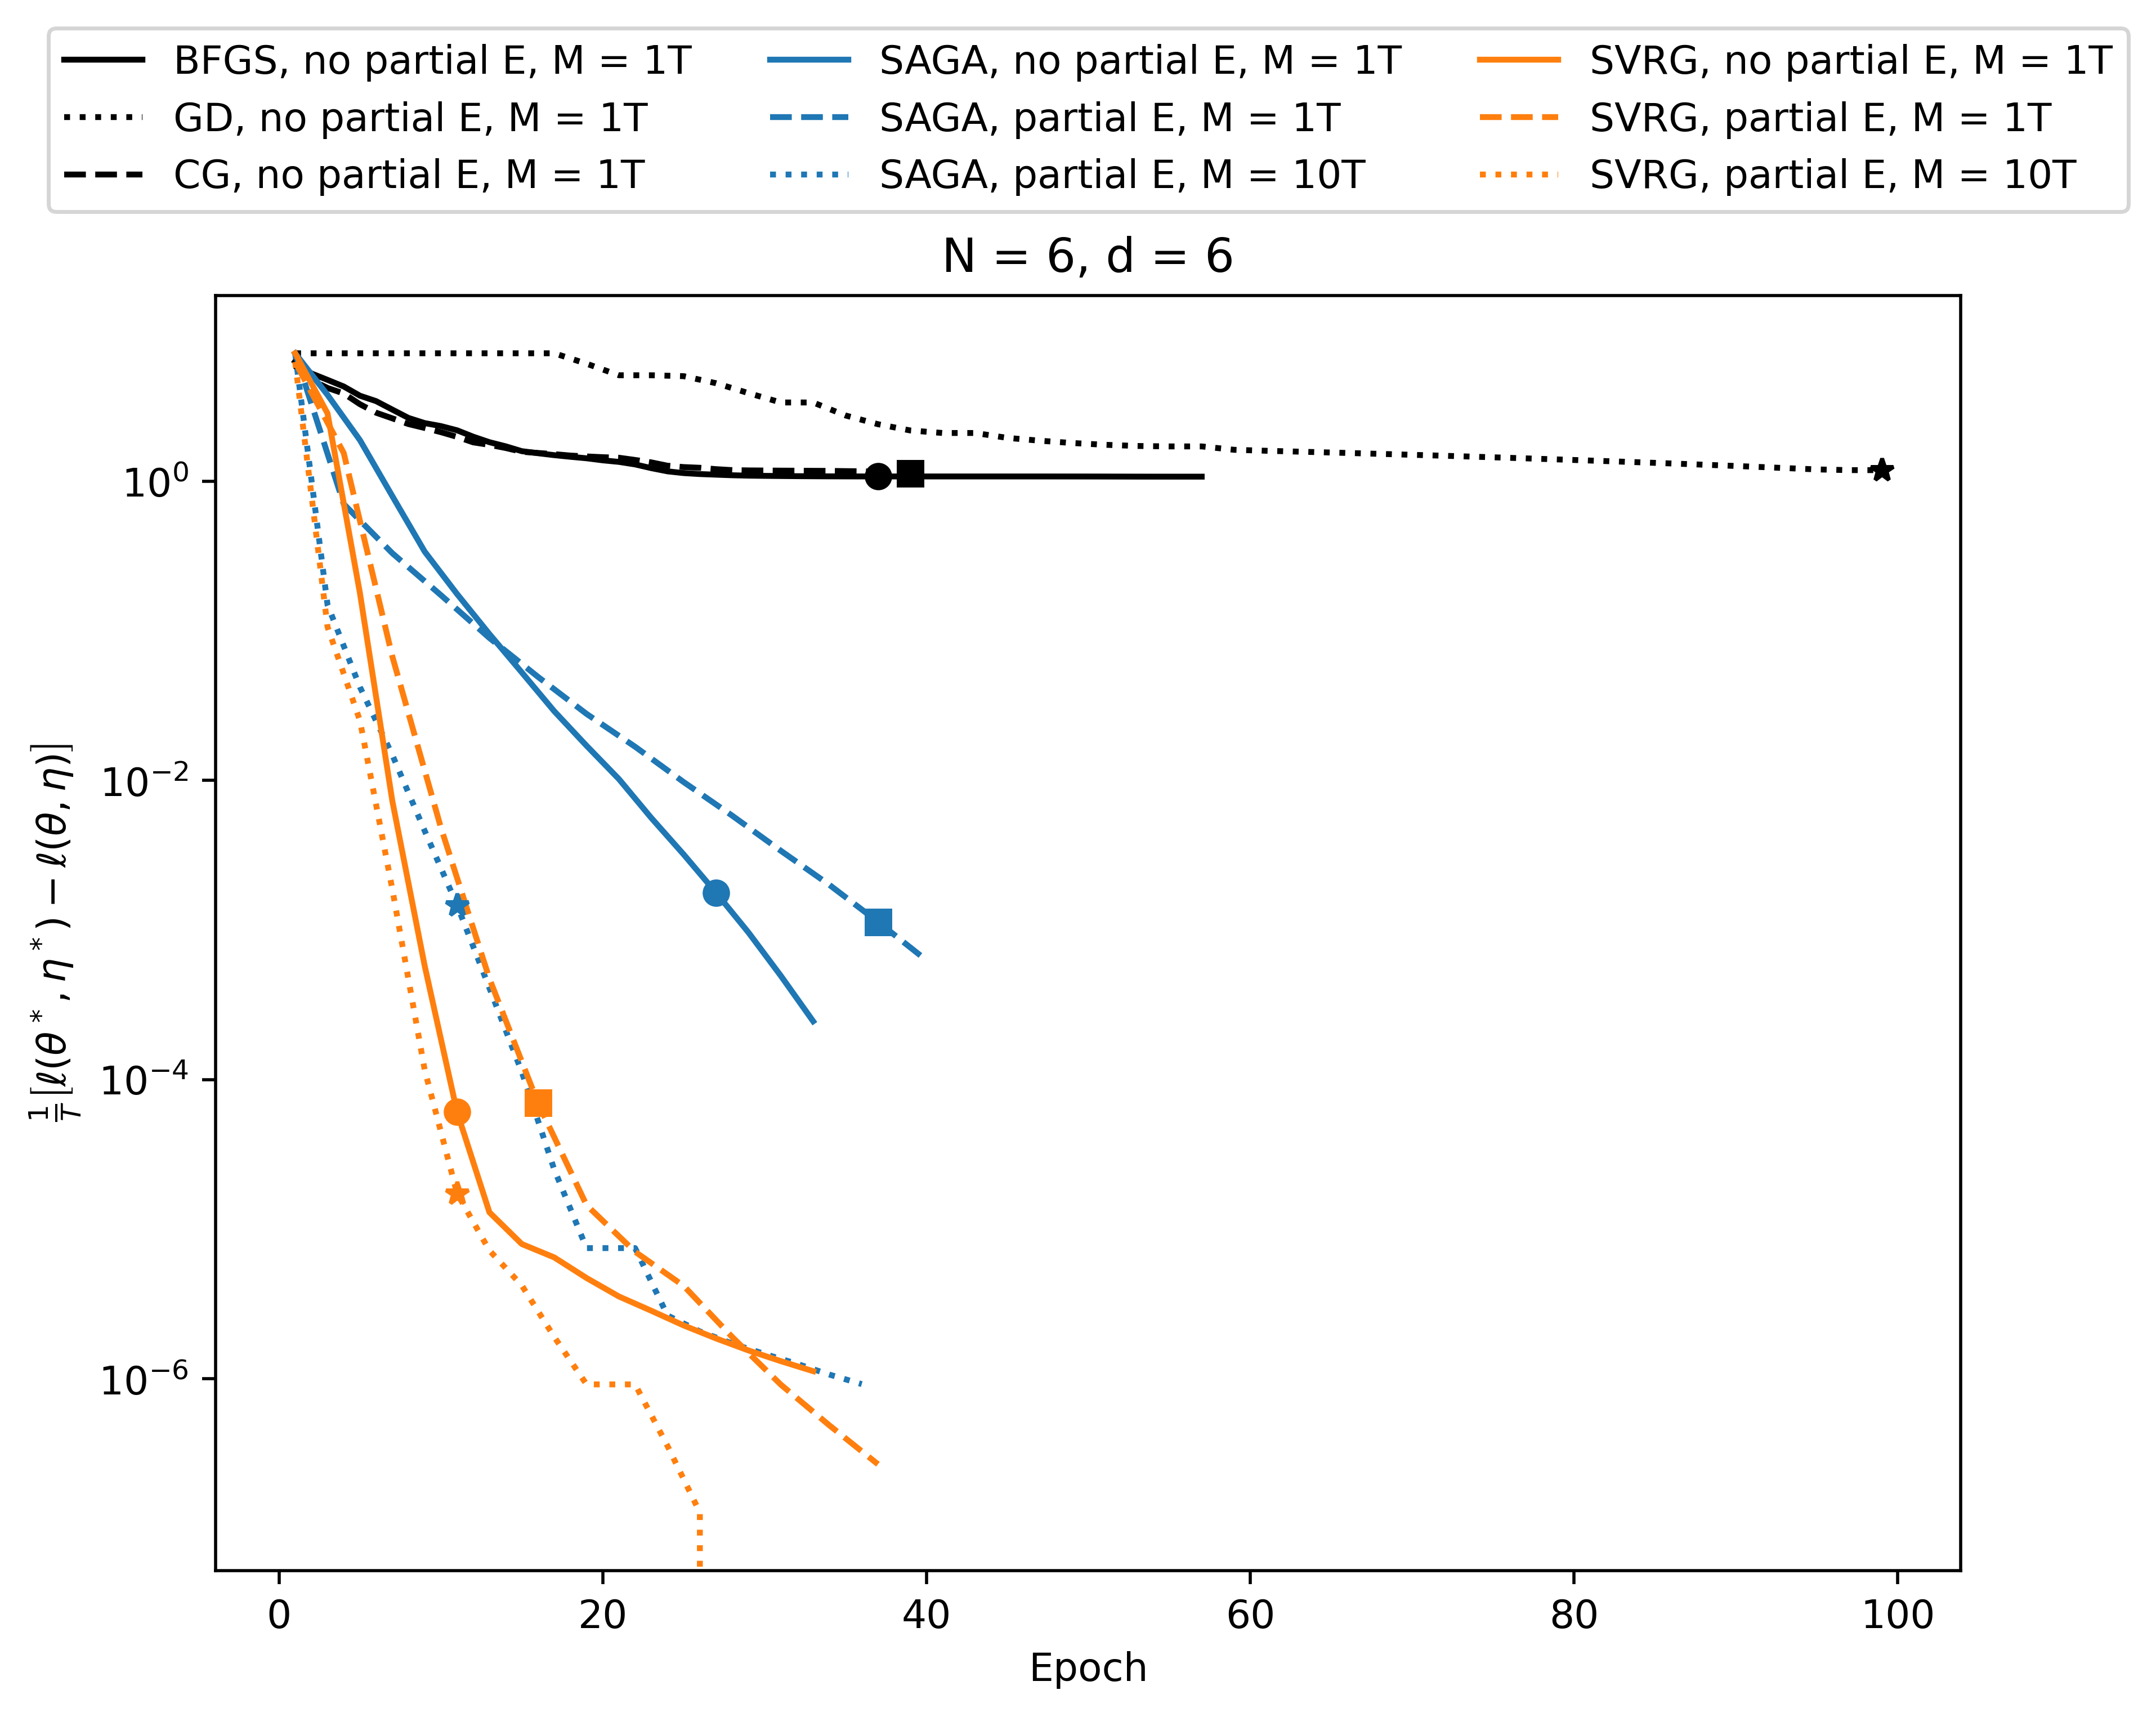
\includegraphics[width=3in]{../plt/log-like_v_epoch_T-100000-K-6-1-d-6-003.png}
    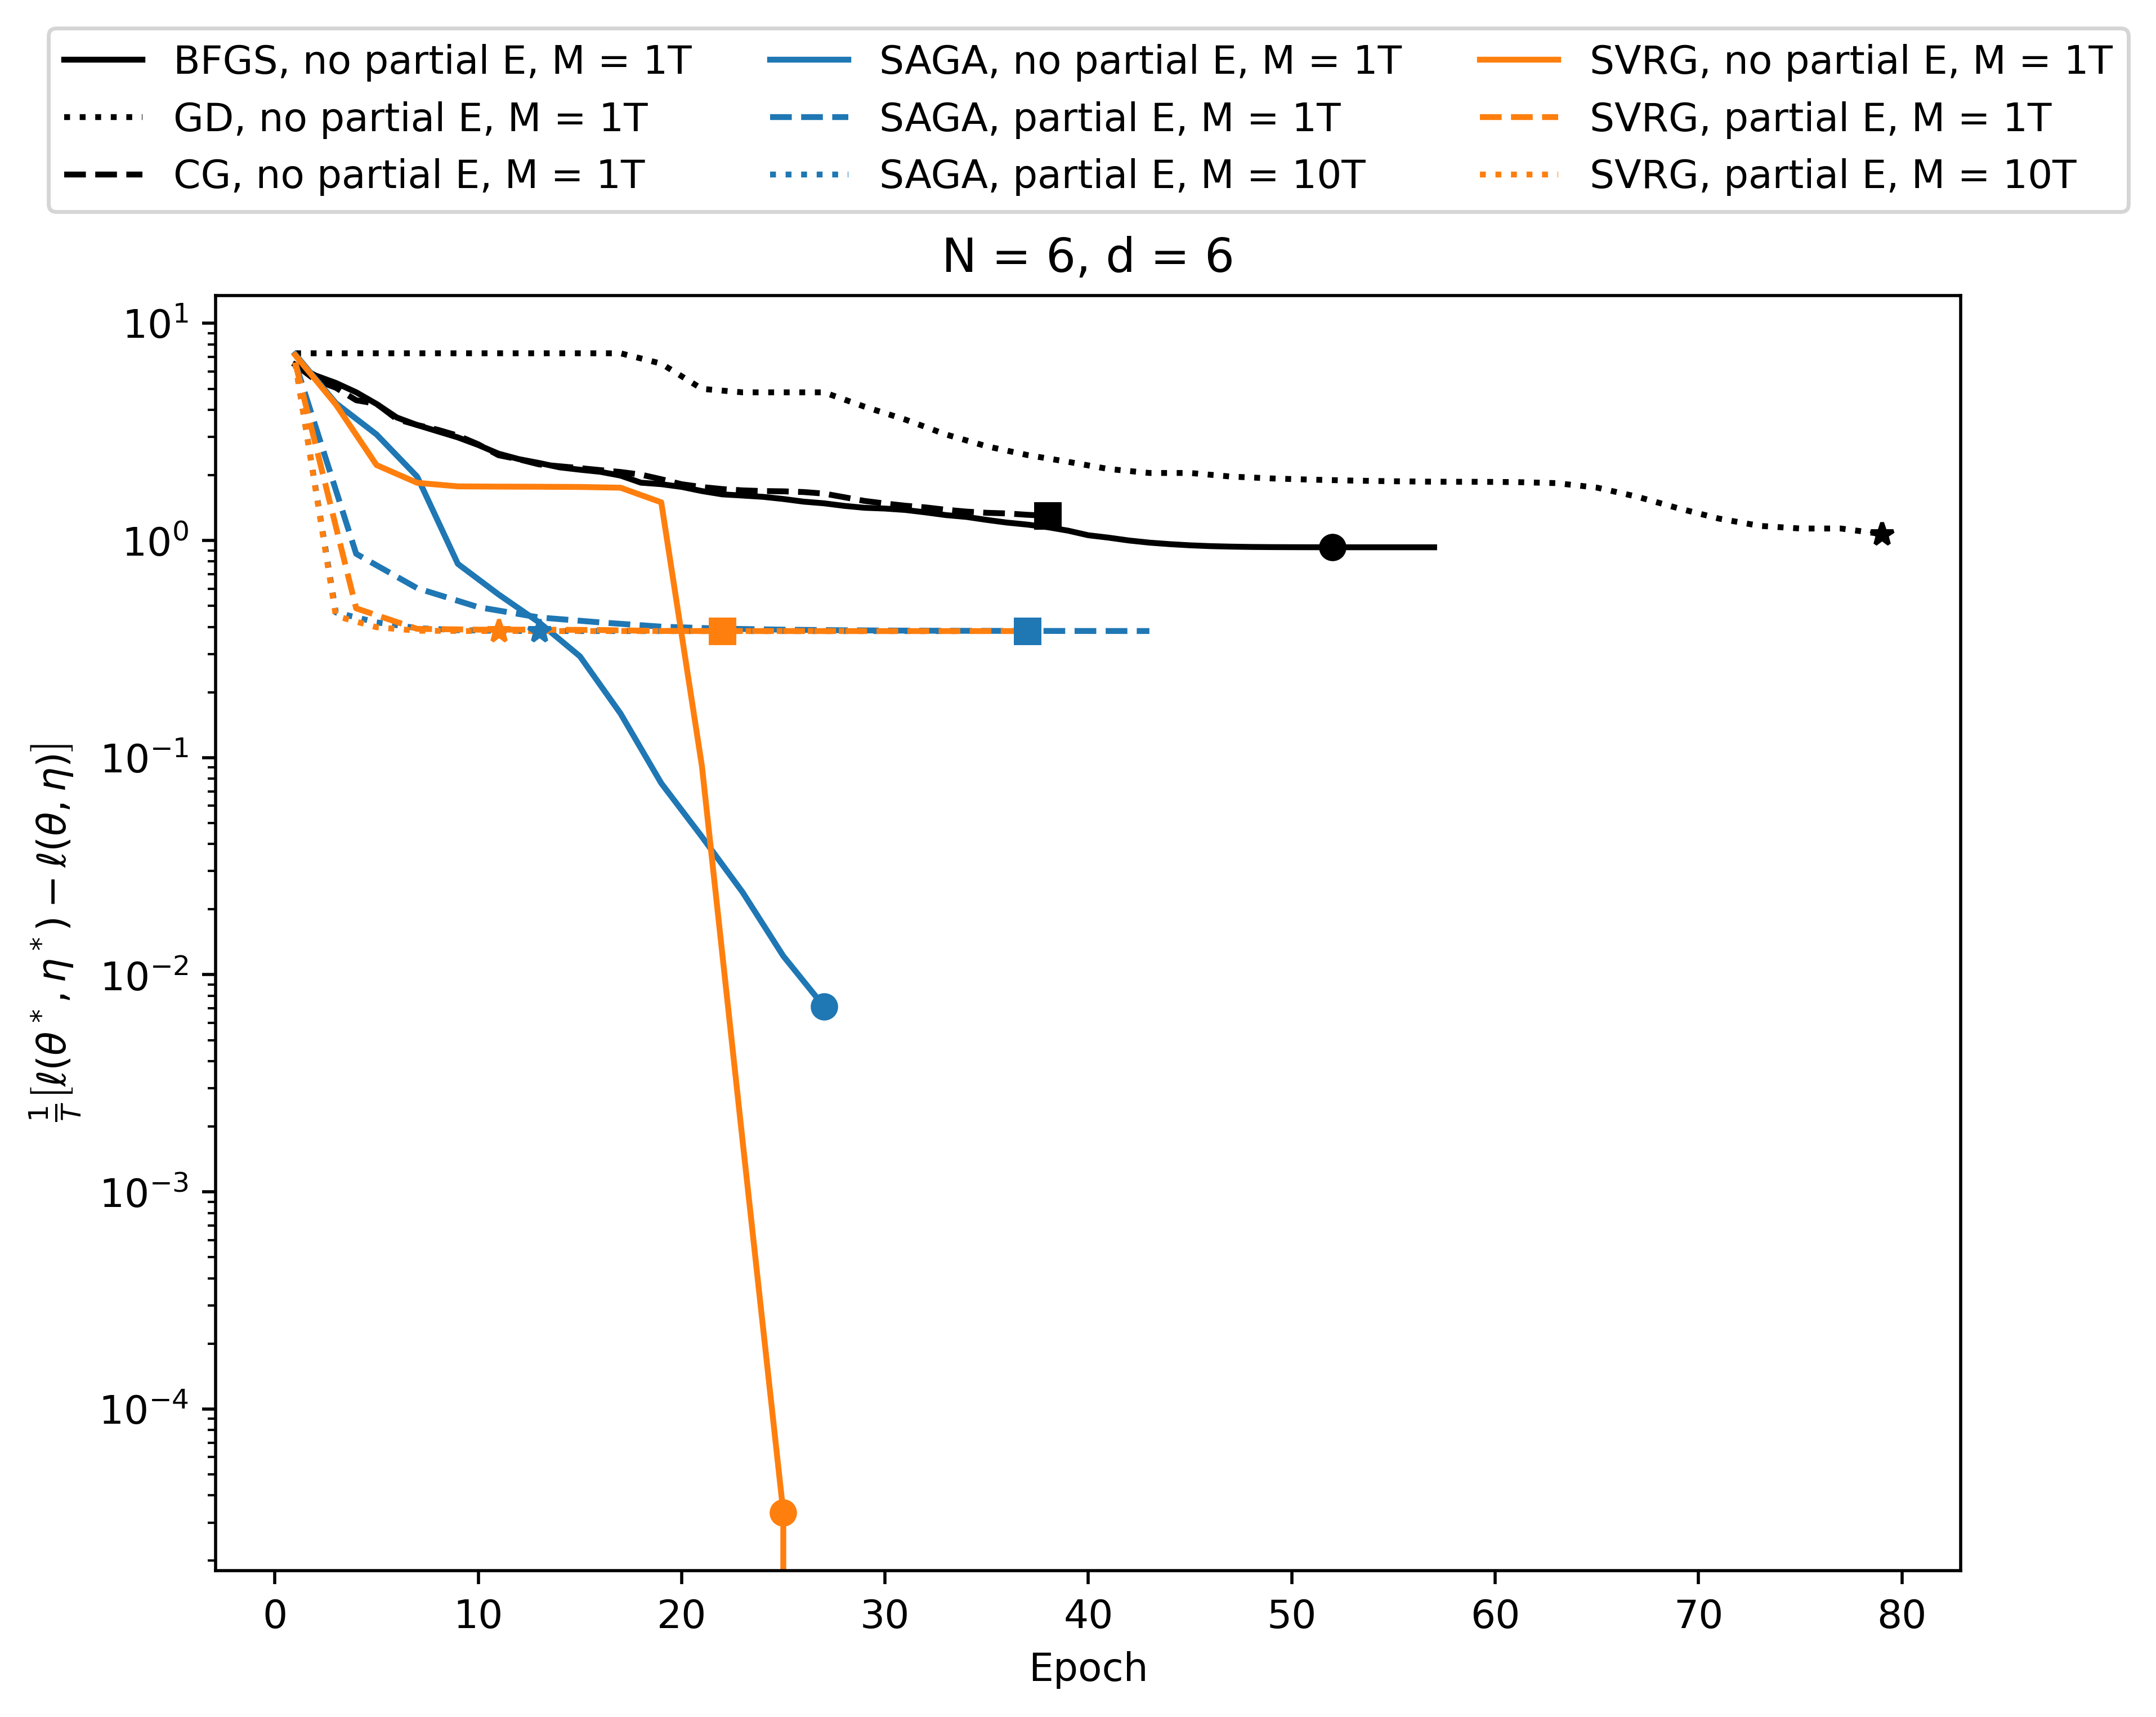
\includegraphics[width=3in]{../plt/log-like_v_epoch_T-100000-K-6-1-d-6-004.png}   
    \caption{Optimally gap between the current log-likelihood and optimal log-likelihood for the simulation studies with $T=10^{5}$, $N=6$ and $d=6$, for four different simulated data sets. One epoch represents either one full E-step, $T$ iterations with the M-step, or one gradient step for full-gradient algorithms. The y-axis is on a log-scale.}
\end{figure}


%%%%%%%%%%%%%%%%%%%%%%%%%%%%%%%%%


\begin{figure}
    \centering
    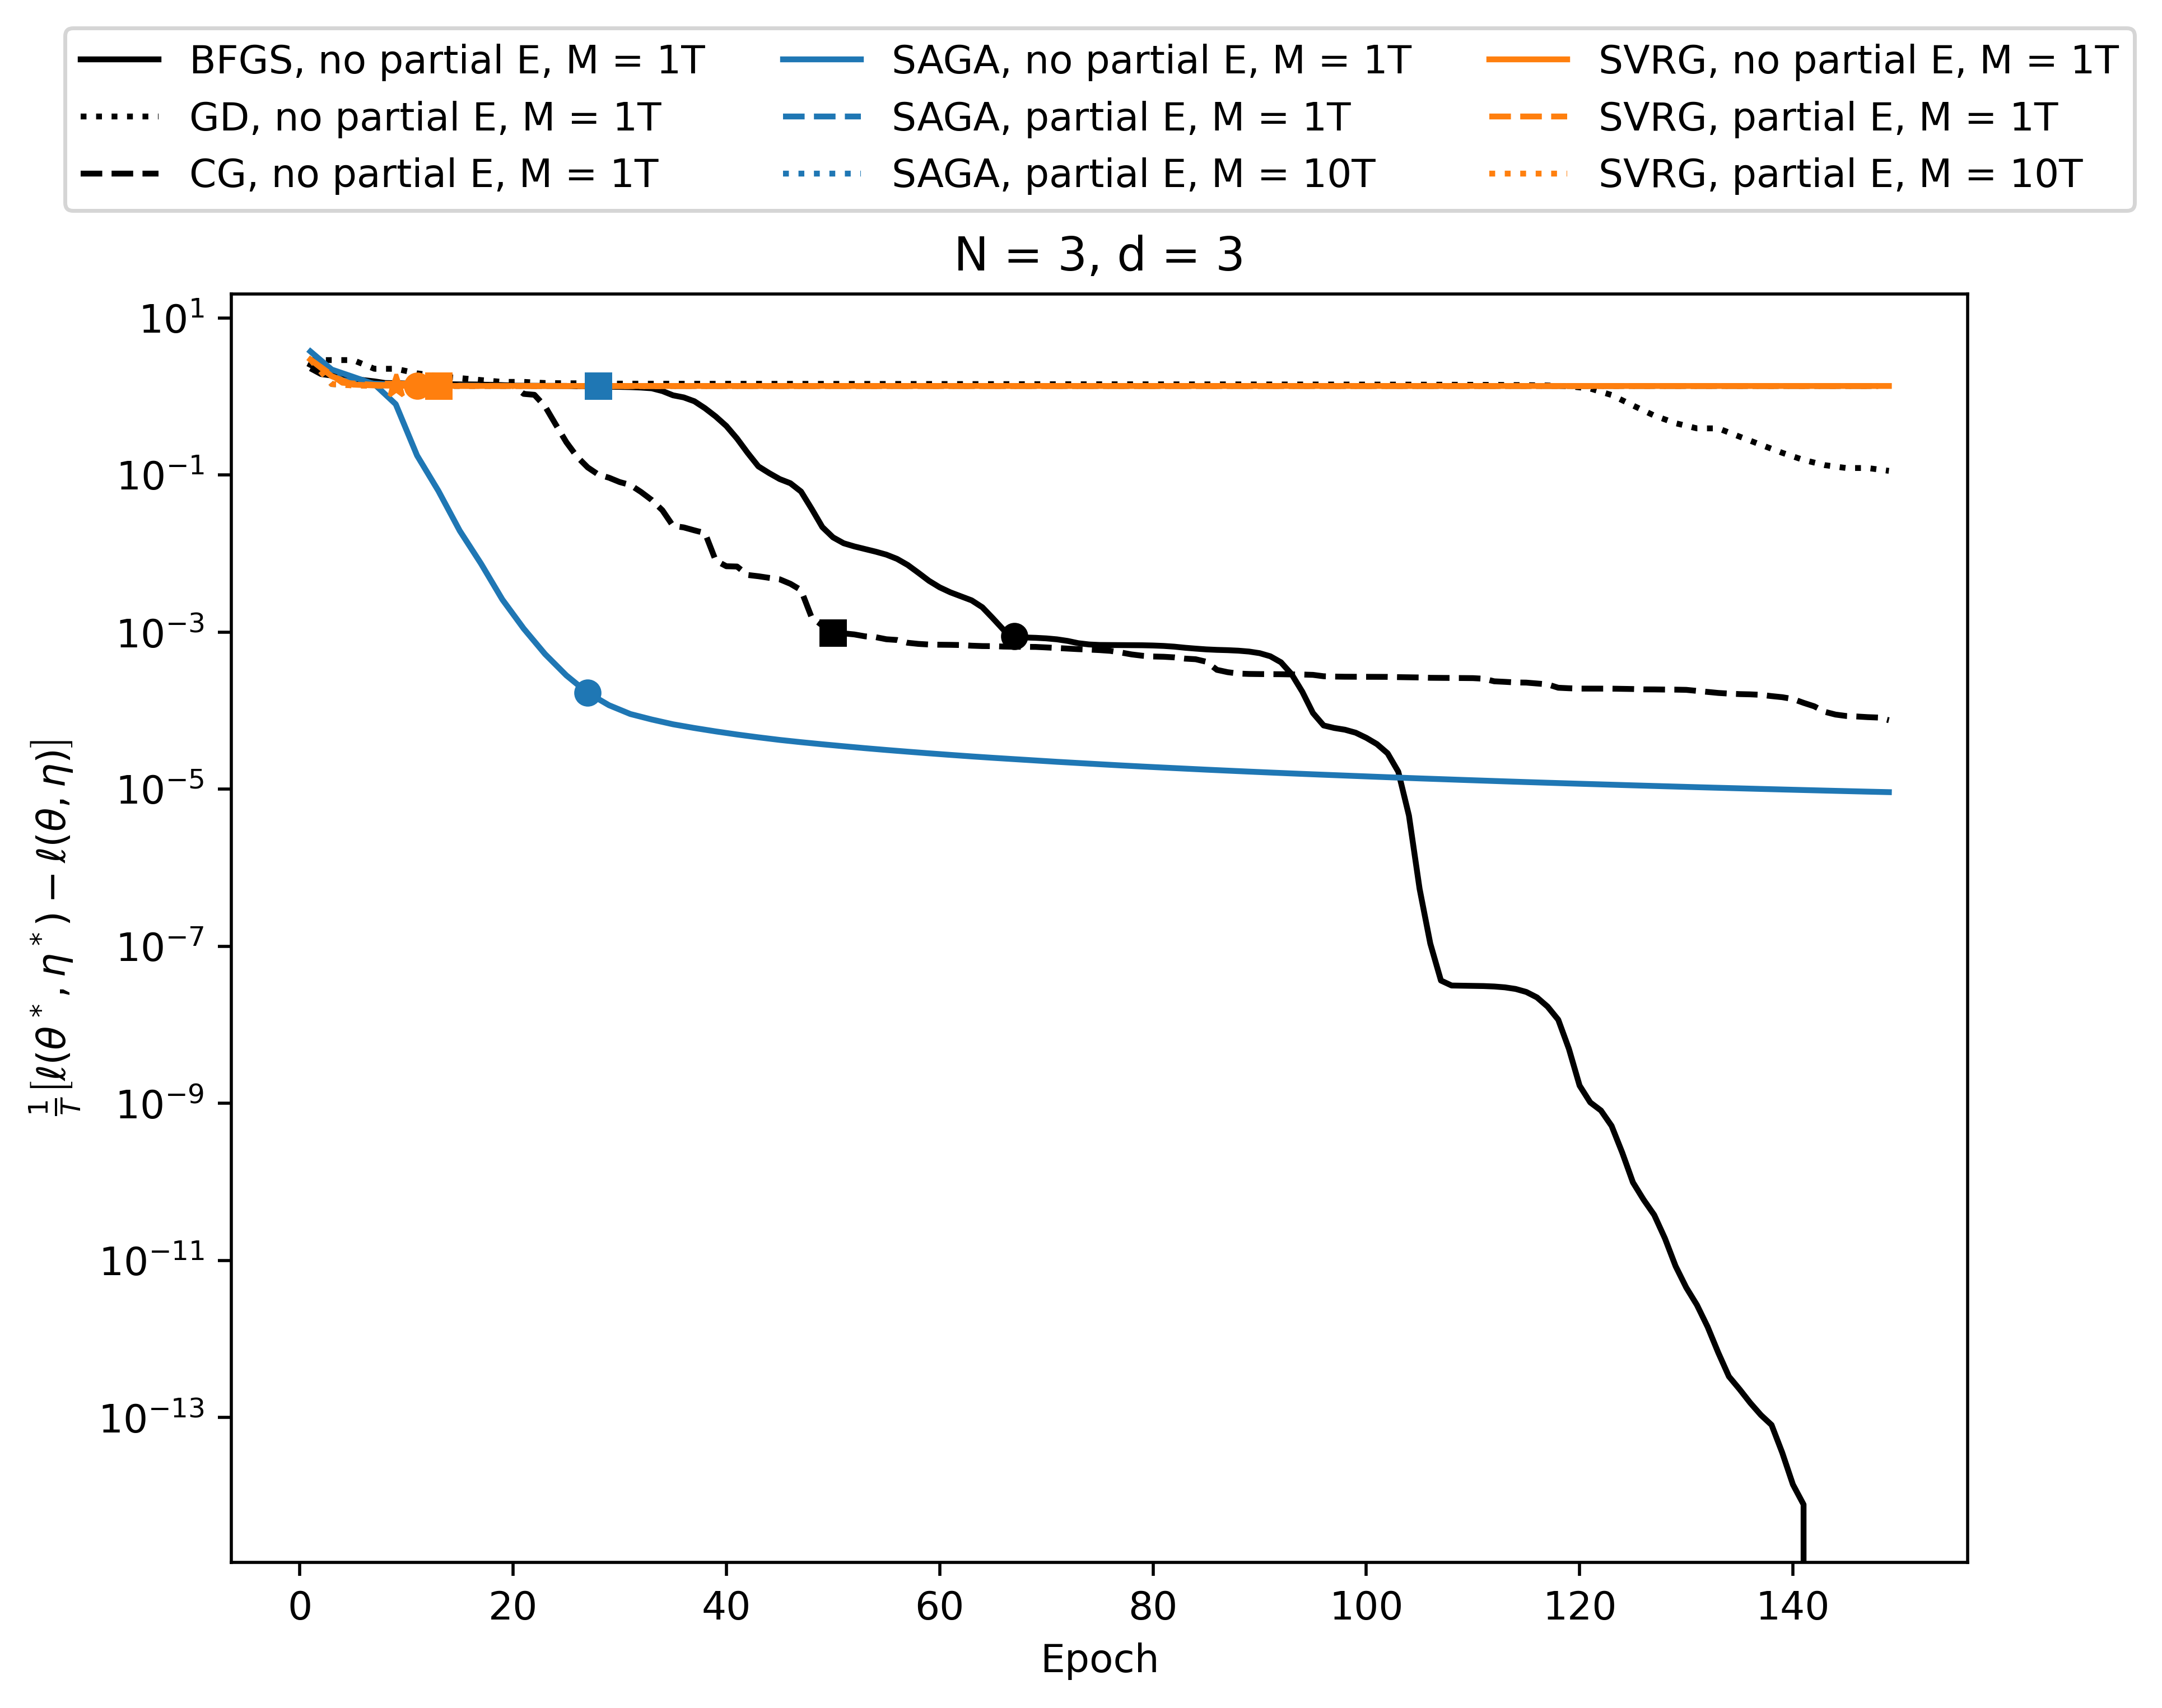
\includegraphics[width=3in]{../plt/log-like_v_epoch_T-1000-K-3-1-d-3-001.png}
    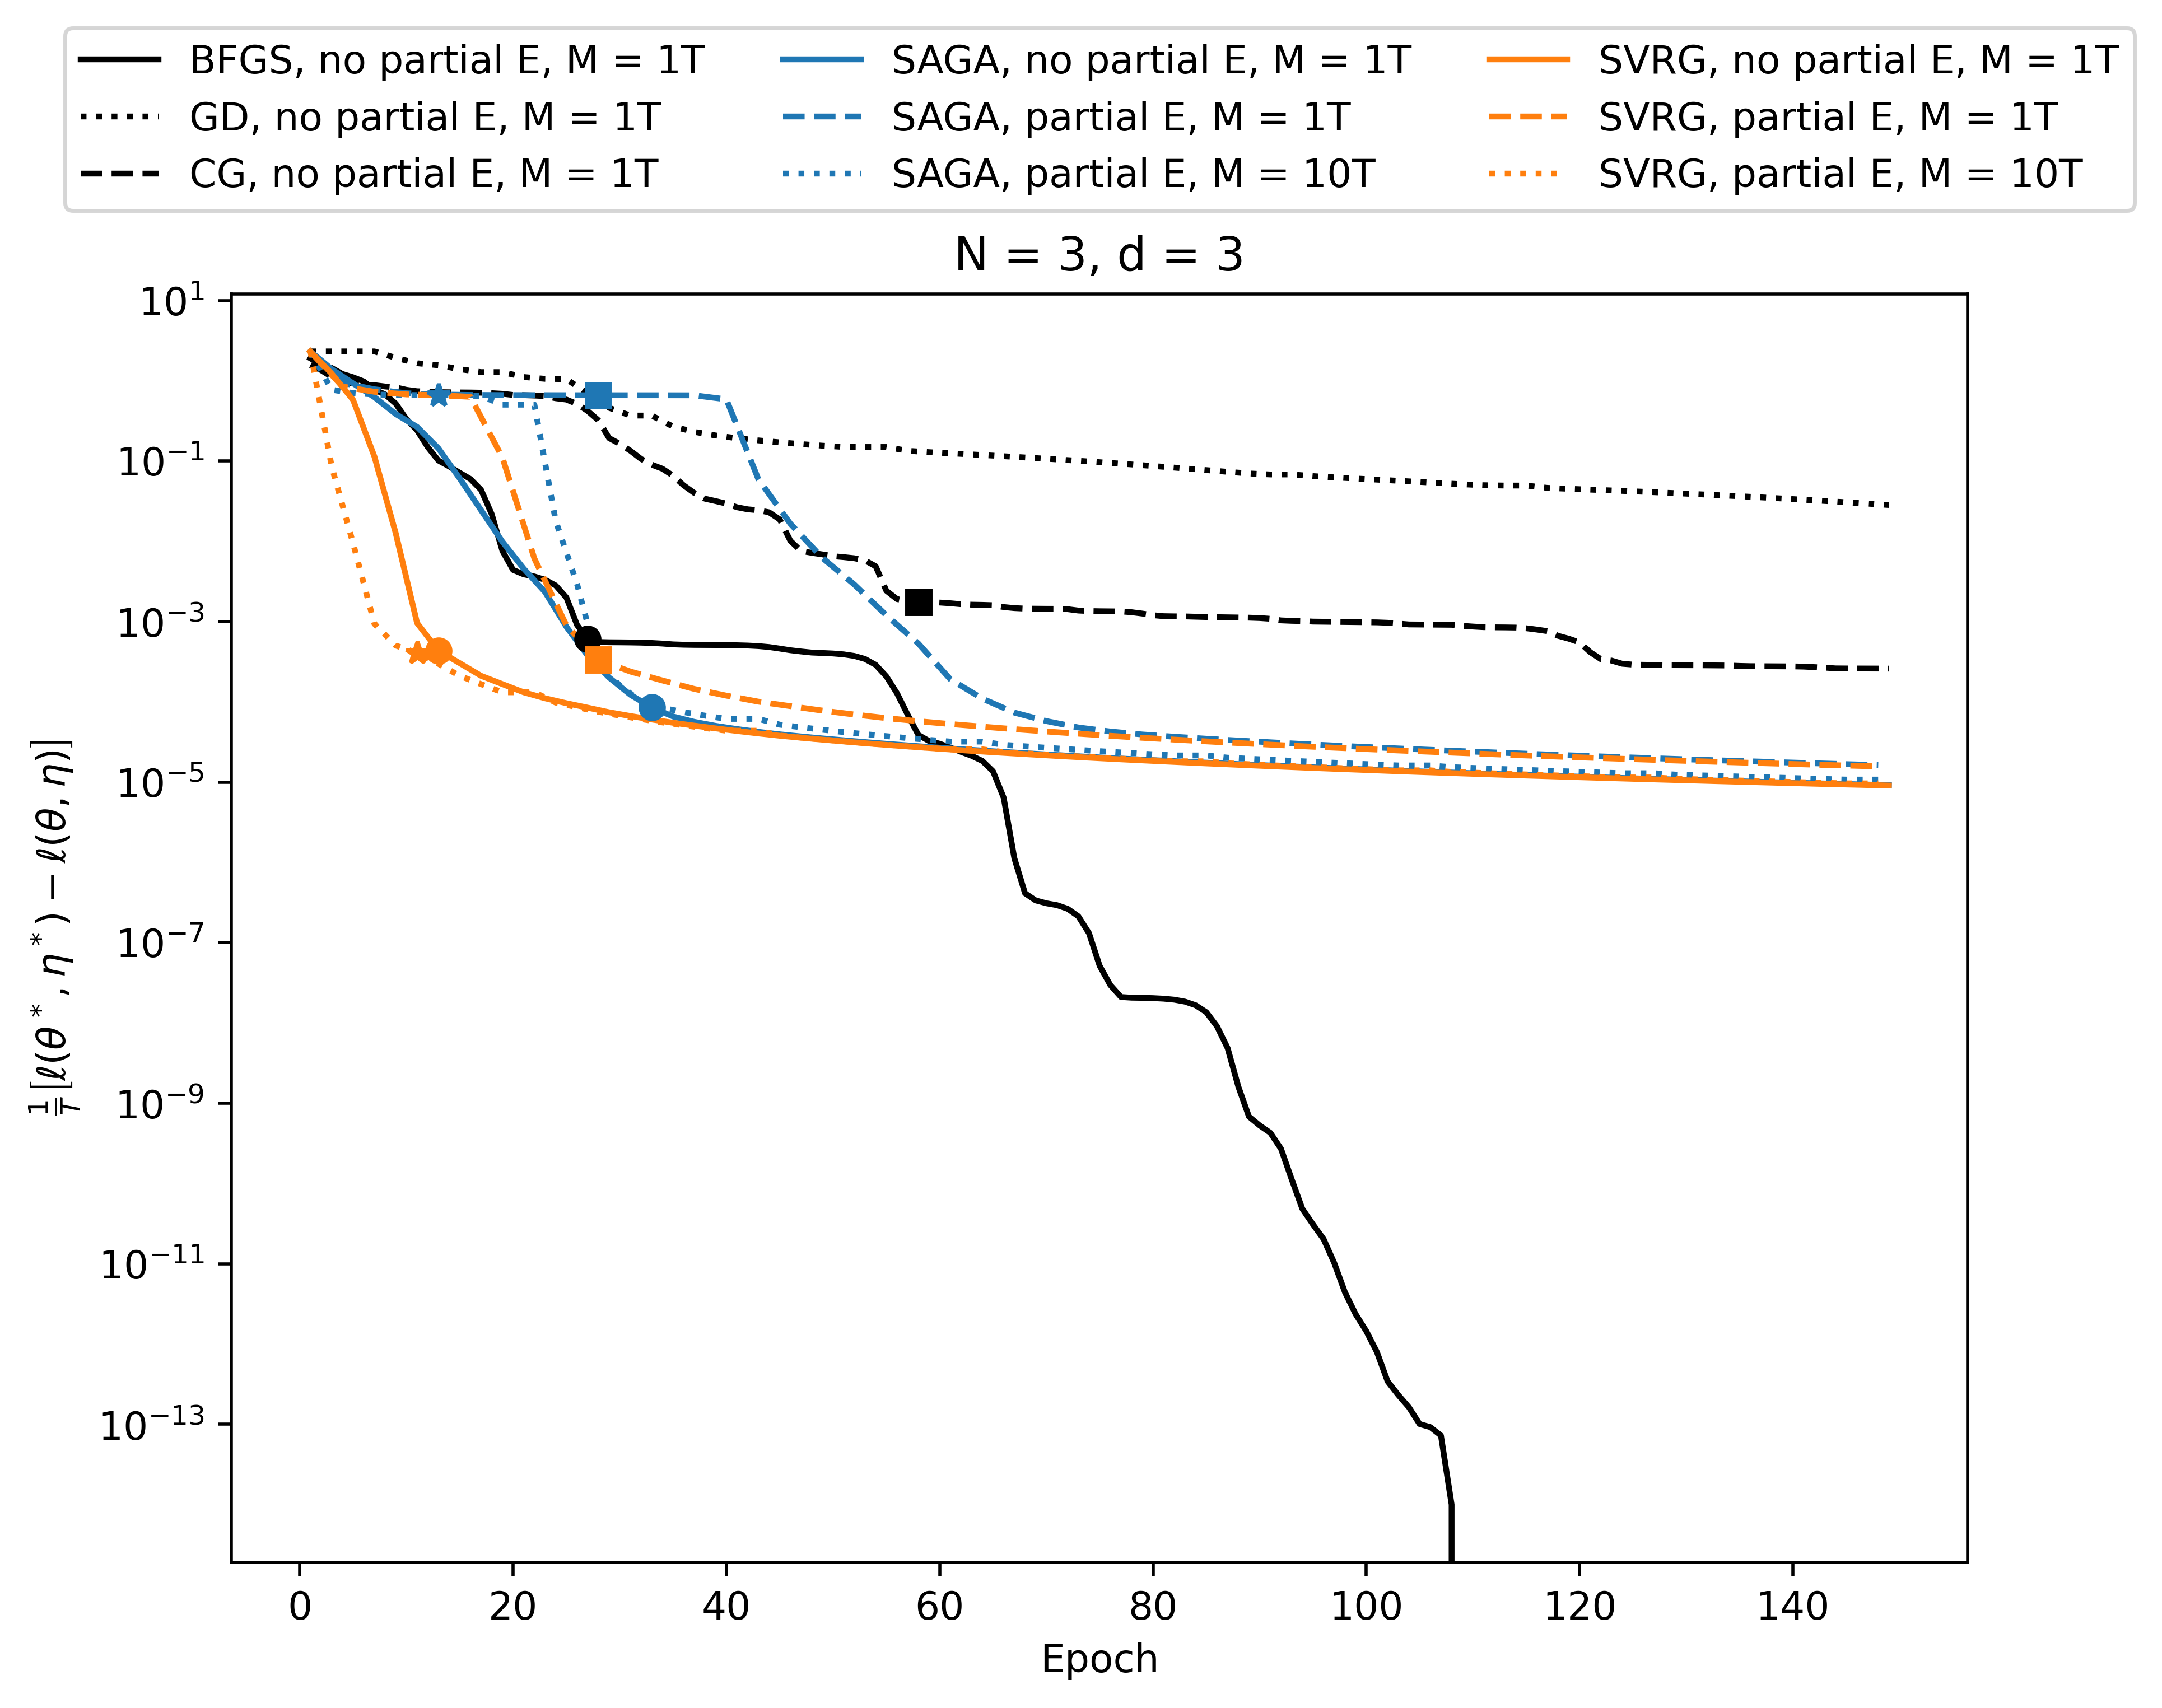
\includegraphics[width=3in]{../plt/log-like_v_epoch_T-1000-K-3-1-d-3-002.png}
    \\
    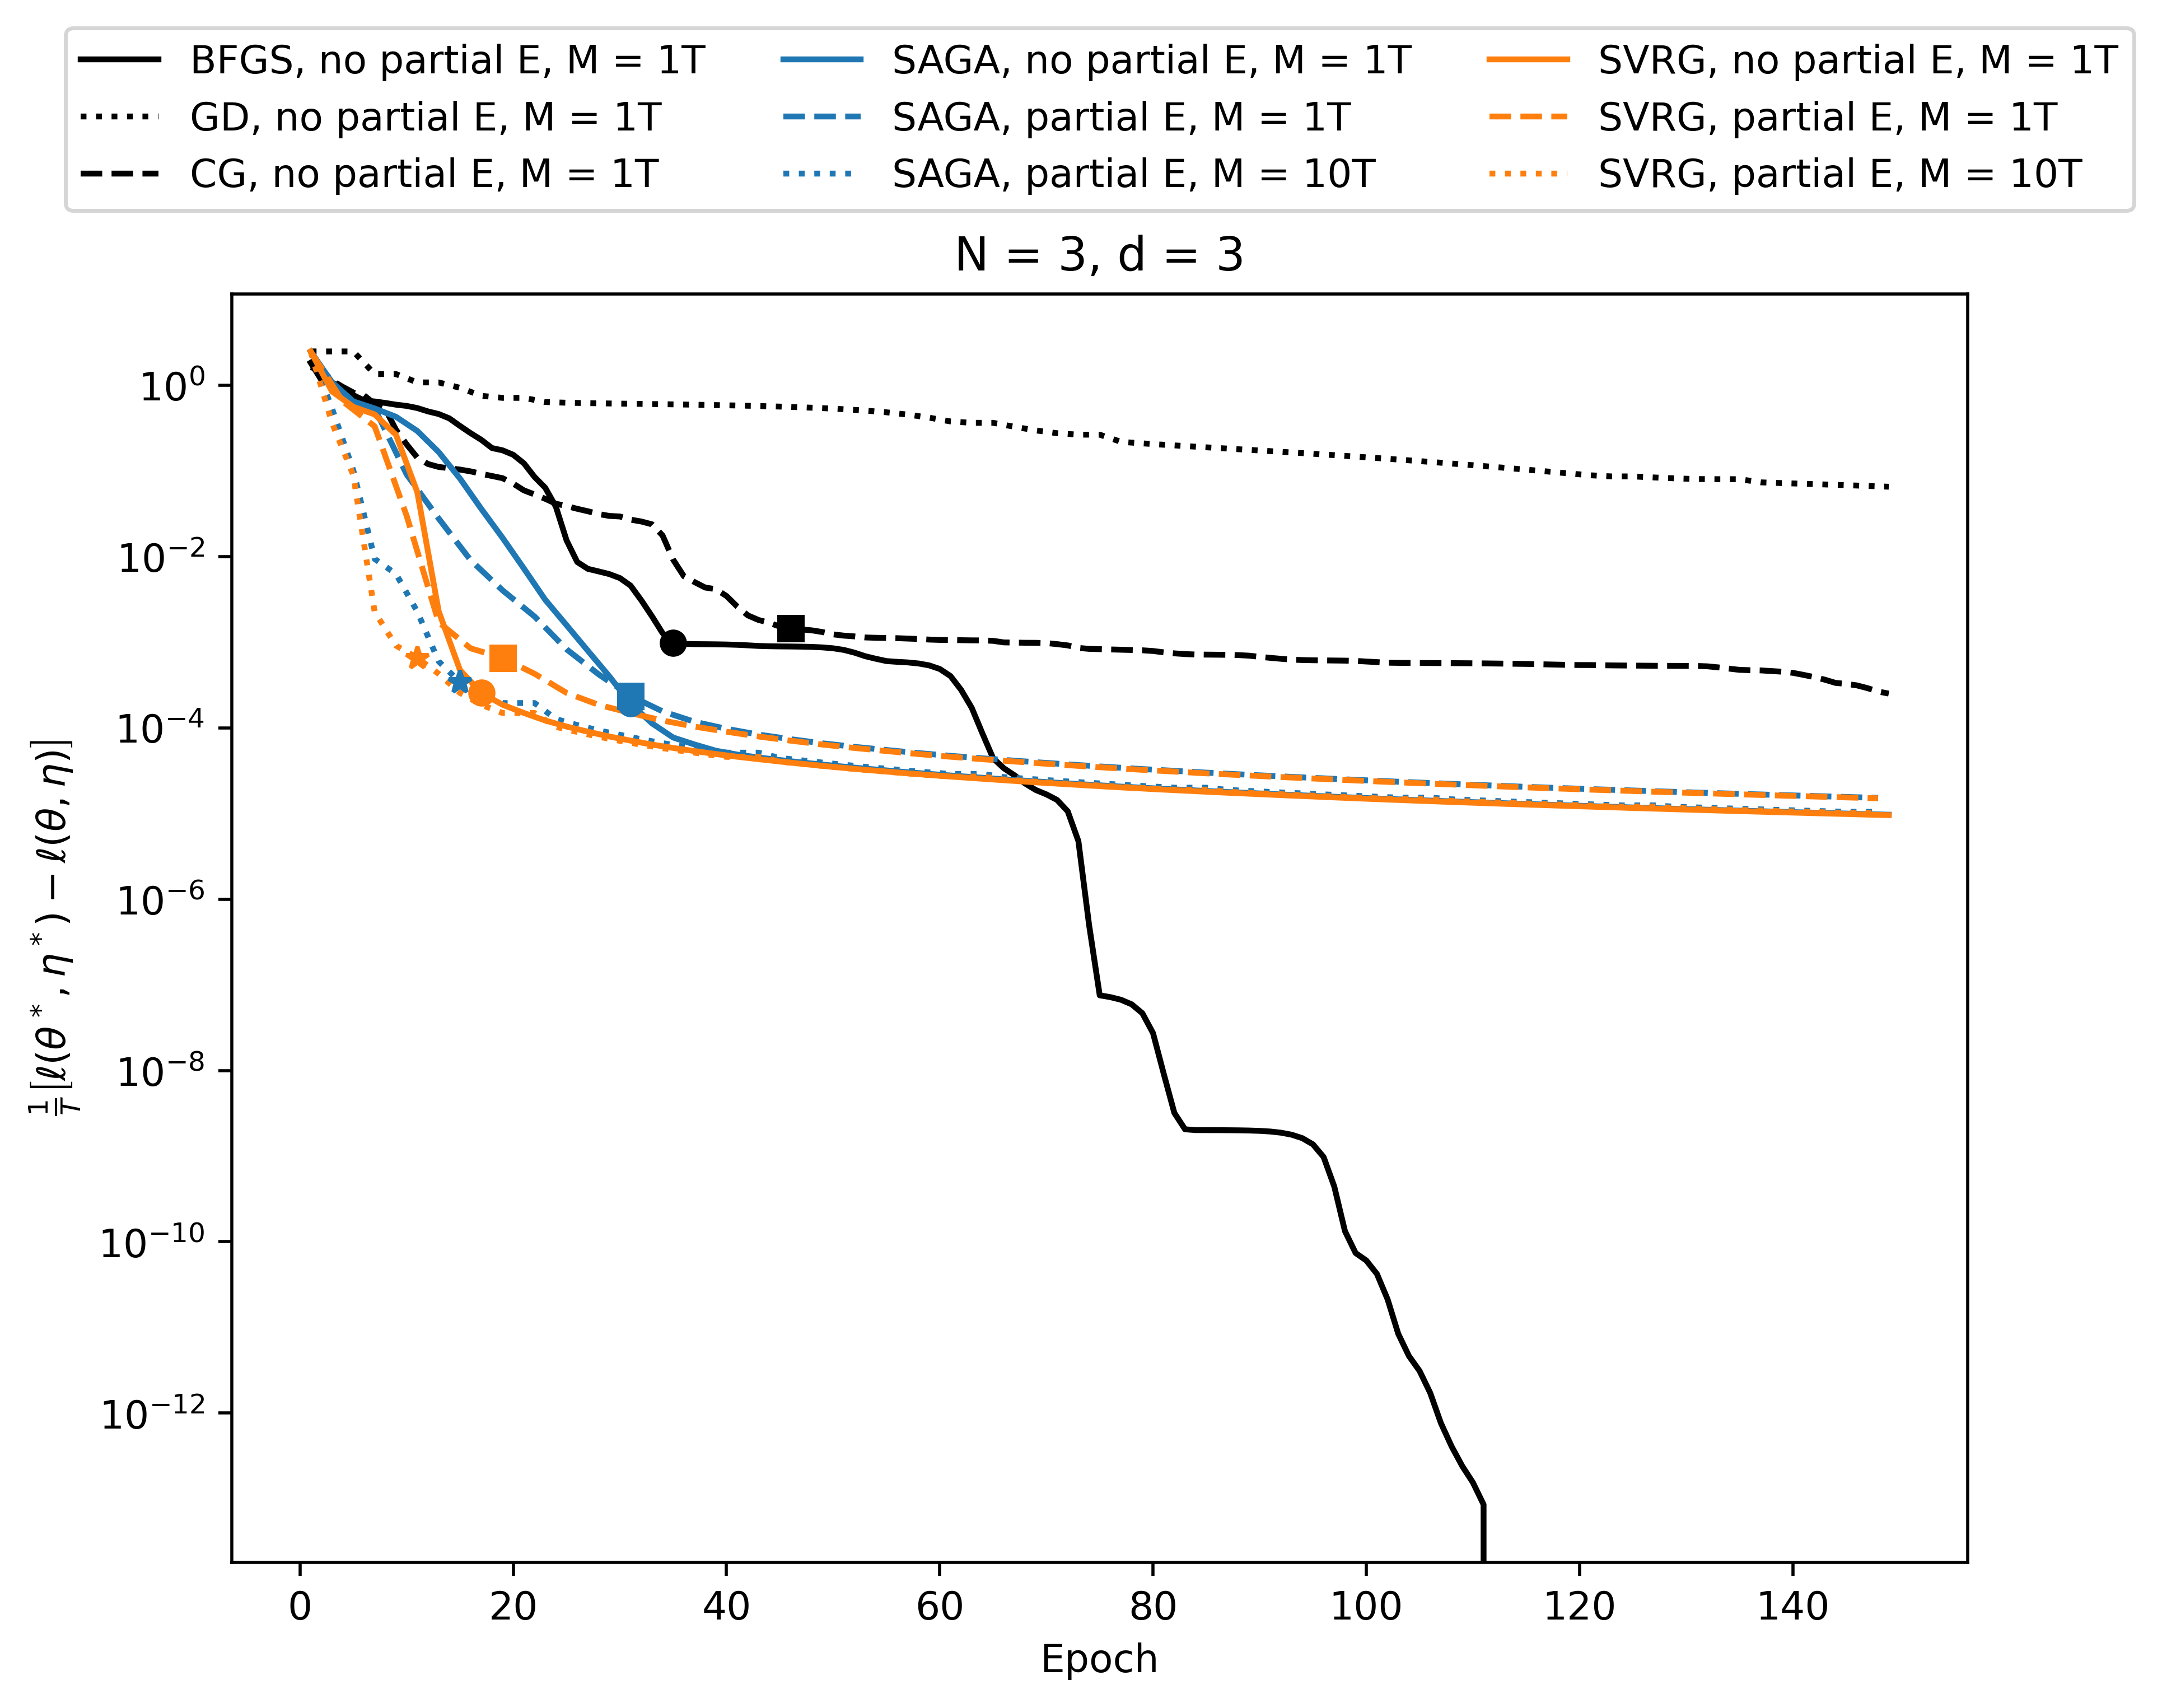
\includegraphics[width=3in]{../plt/log-like_v_epoch_T-1000-K-3-1-d-3-003.png}
    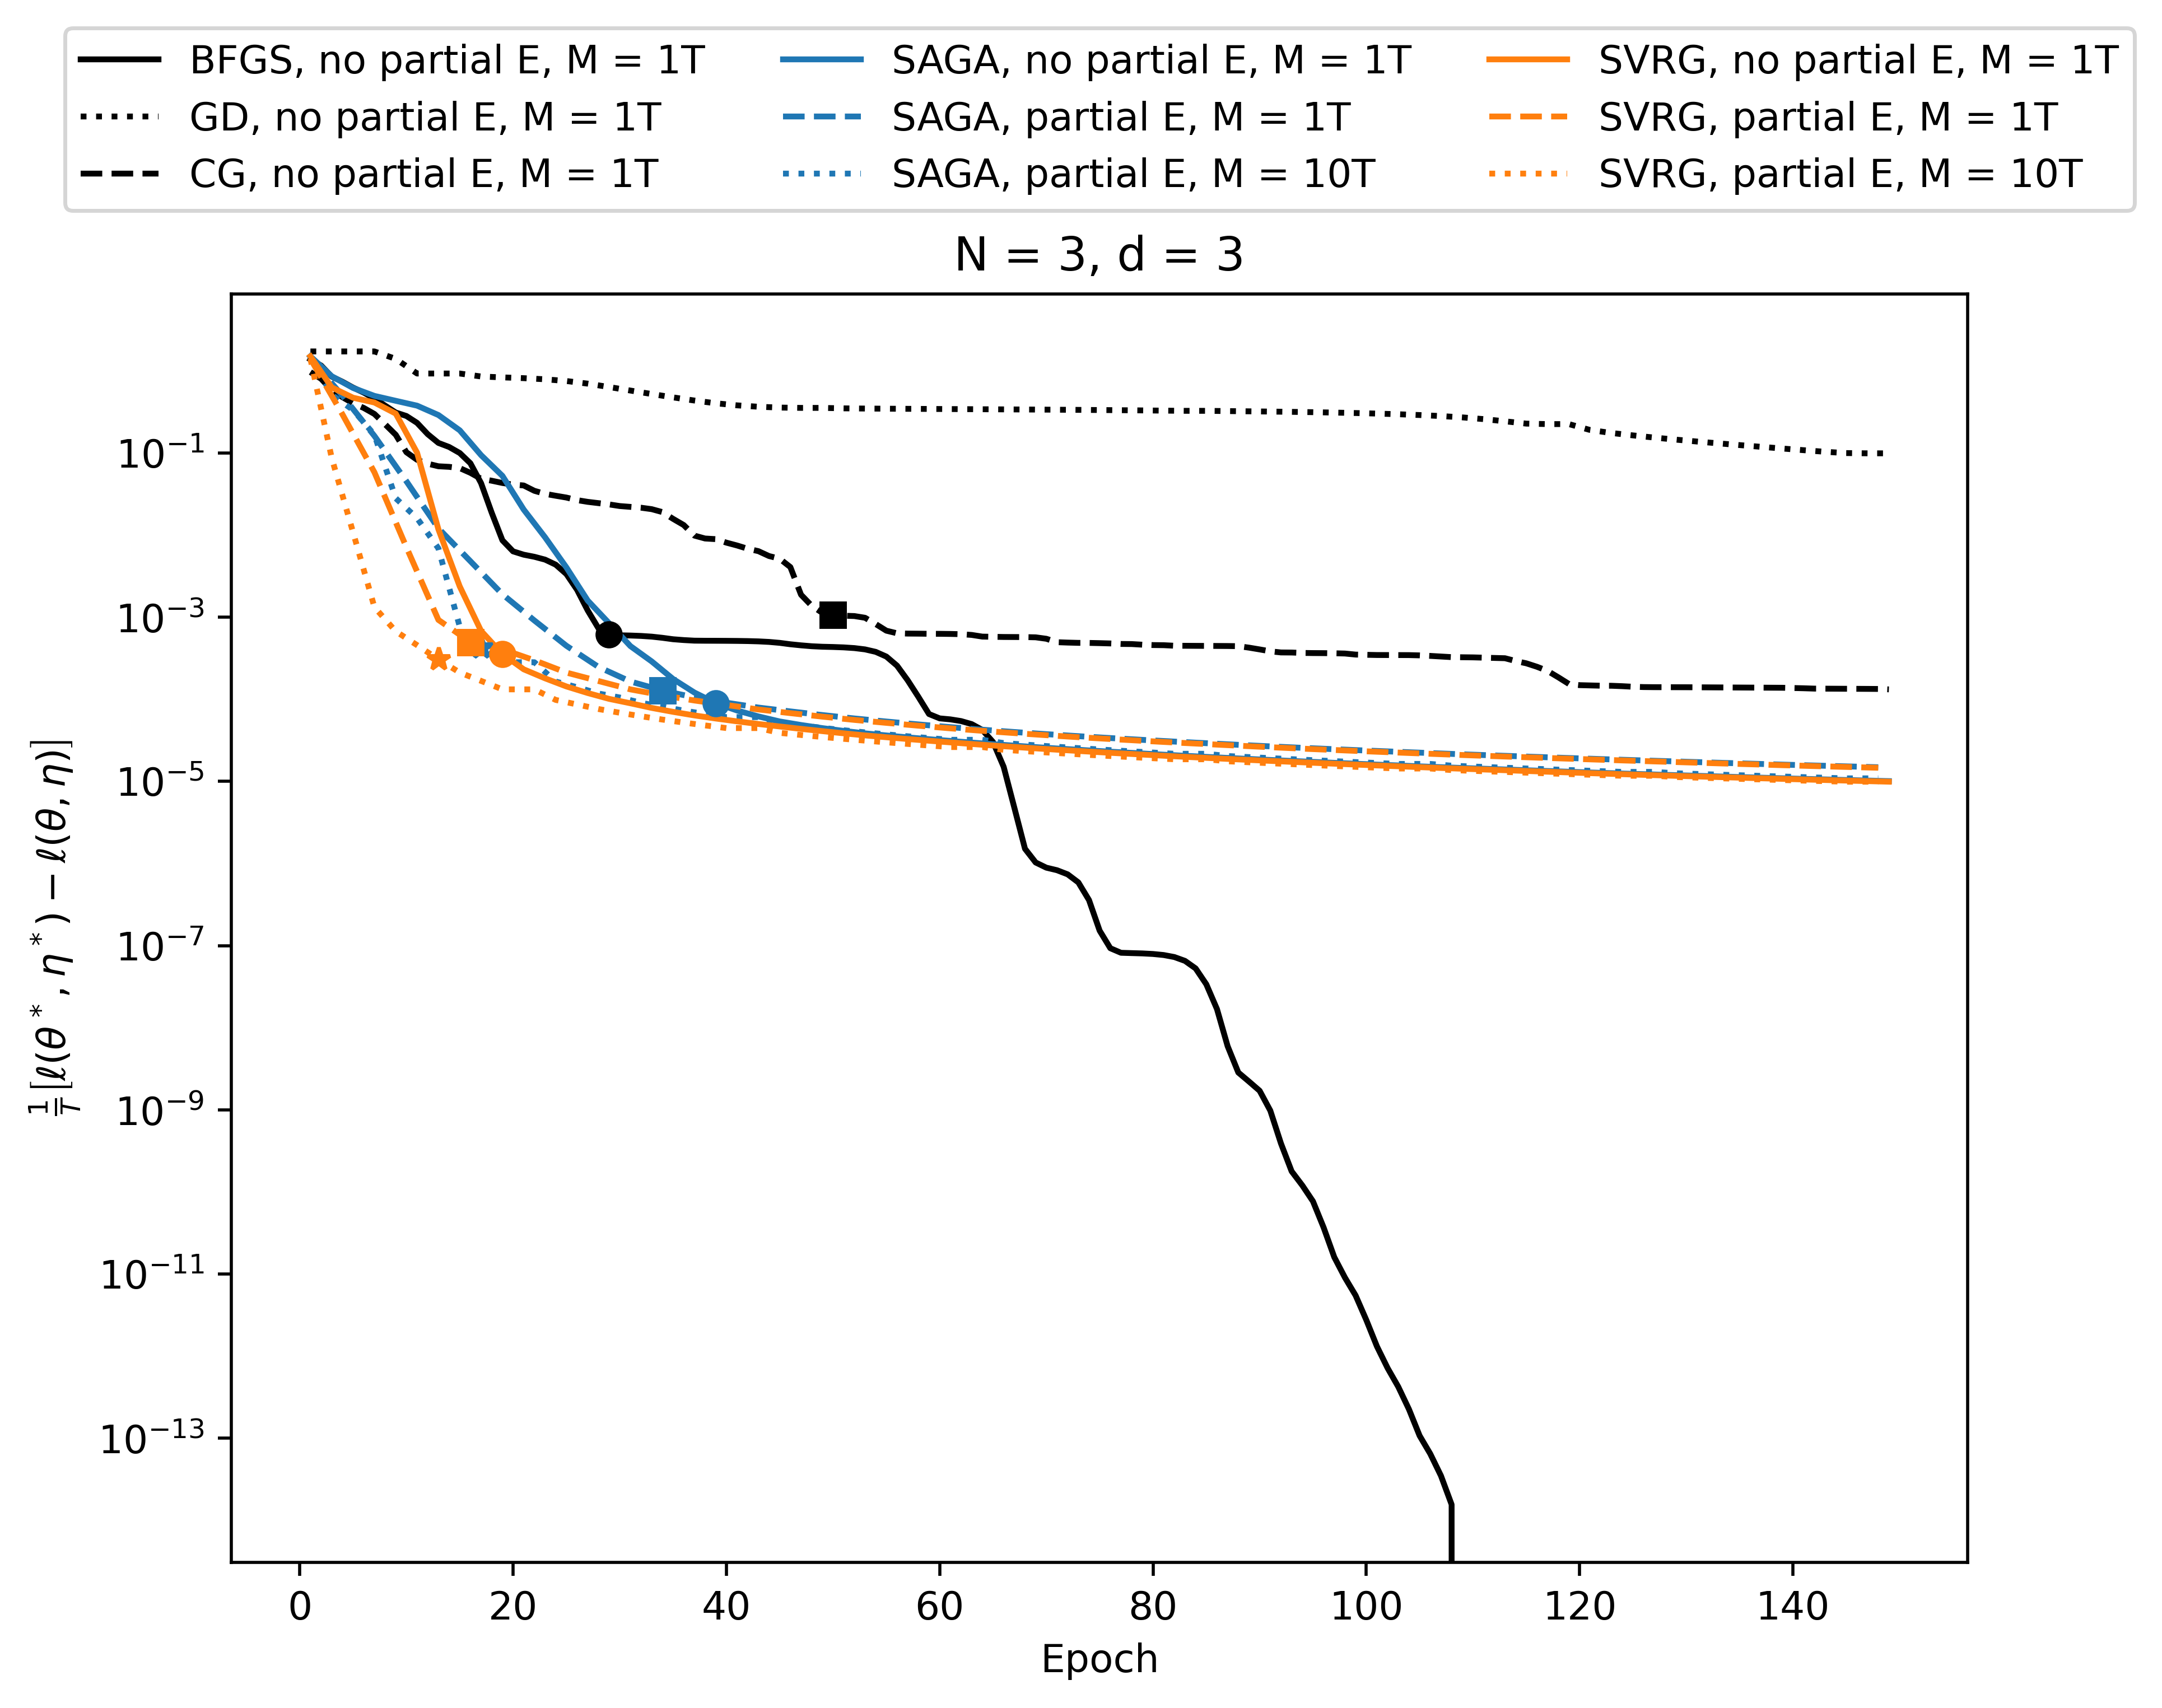
\includegraphics[width=3in]{../plt/log-like_v_epoch_T-1000-K-3-1-d-3-004.png}   
    \caption{Optimally gap between the current log-likelihood and optimal log-likelihood for the simulation studies with $T=10^{3}$, $N=3$ and $d=3$, for four different simulated data sets. One epoch represents either one full E-step, $T$ iterations with the M-step, or one gradient step for full-gradient algorithms. The y-axis is on a log-scale.}
\end{figure}
%
\begin{figure}
    \centering
    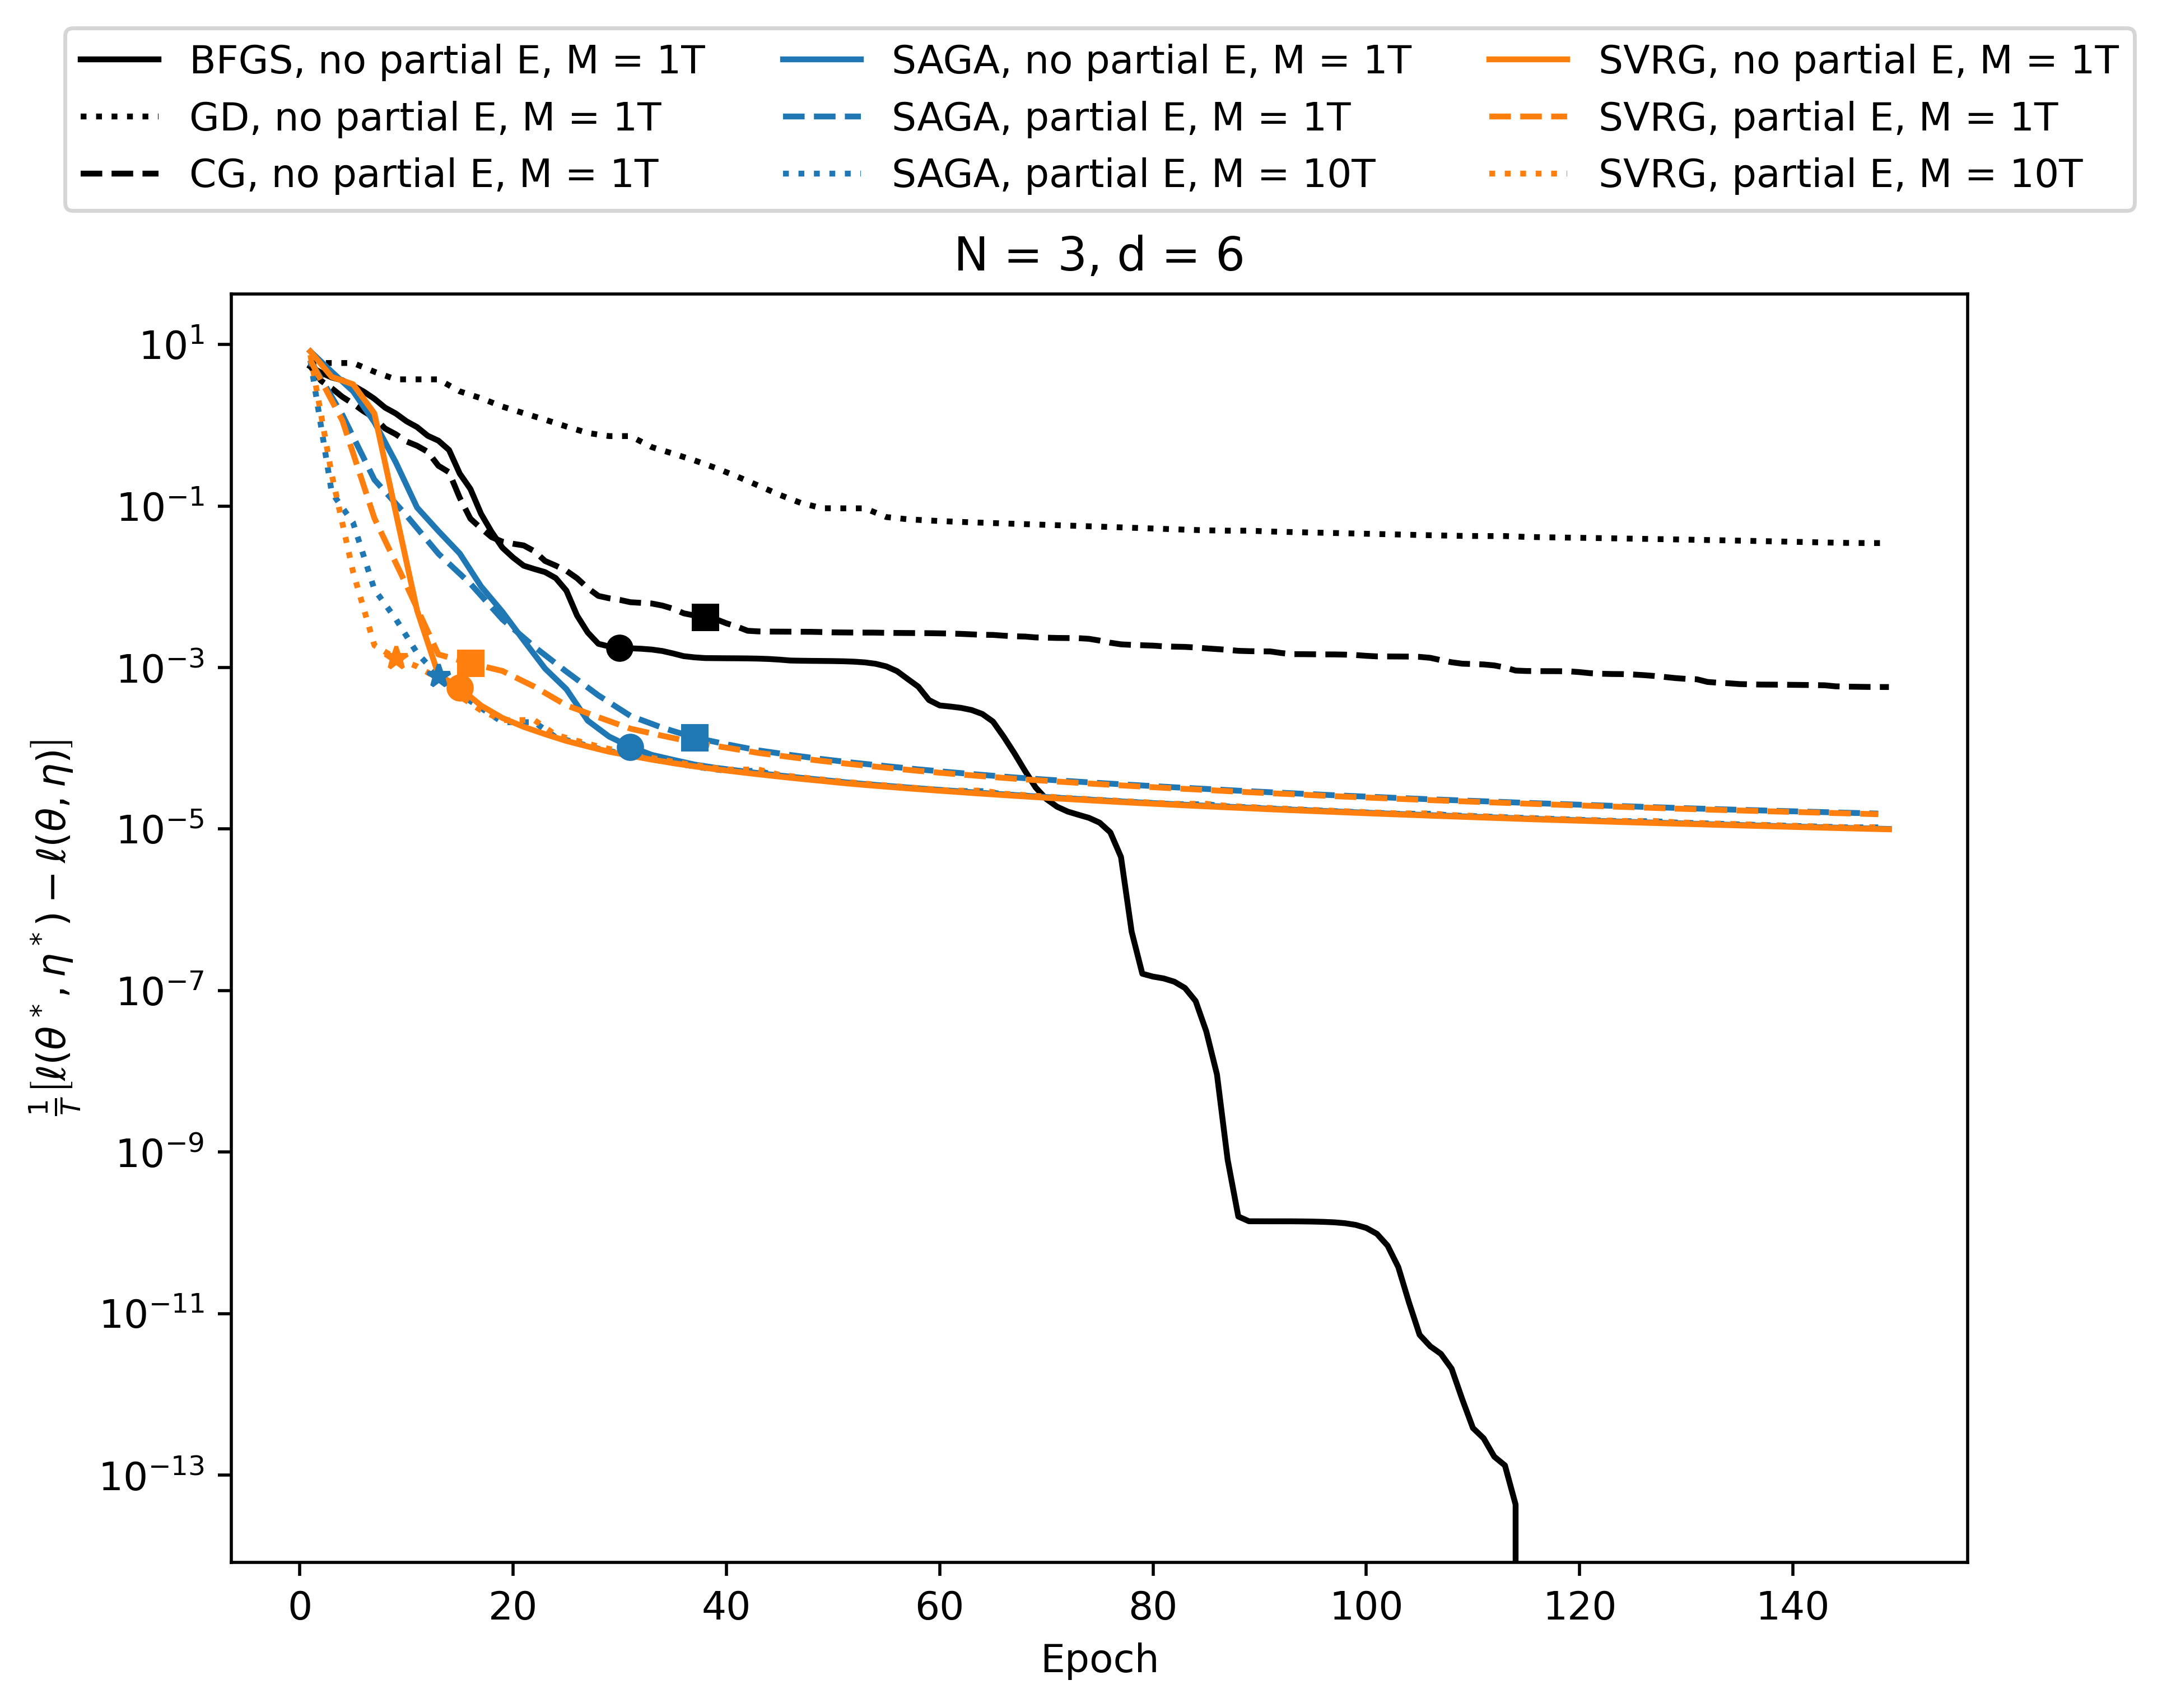
\includegraphics[width=3in]{../plt/log-like_v_epoch_T-1000-K-3-1-d-6-001.png}
    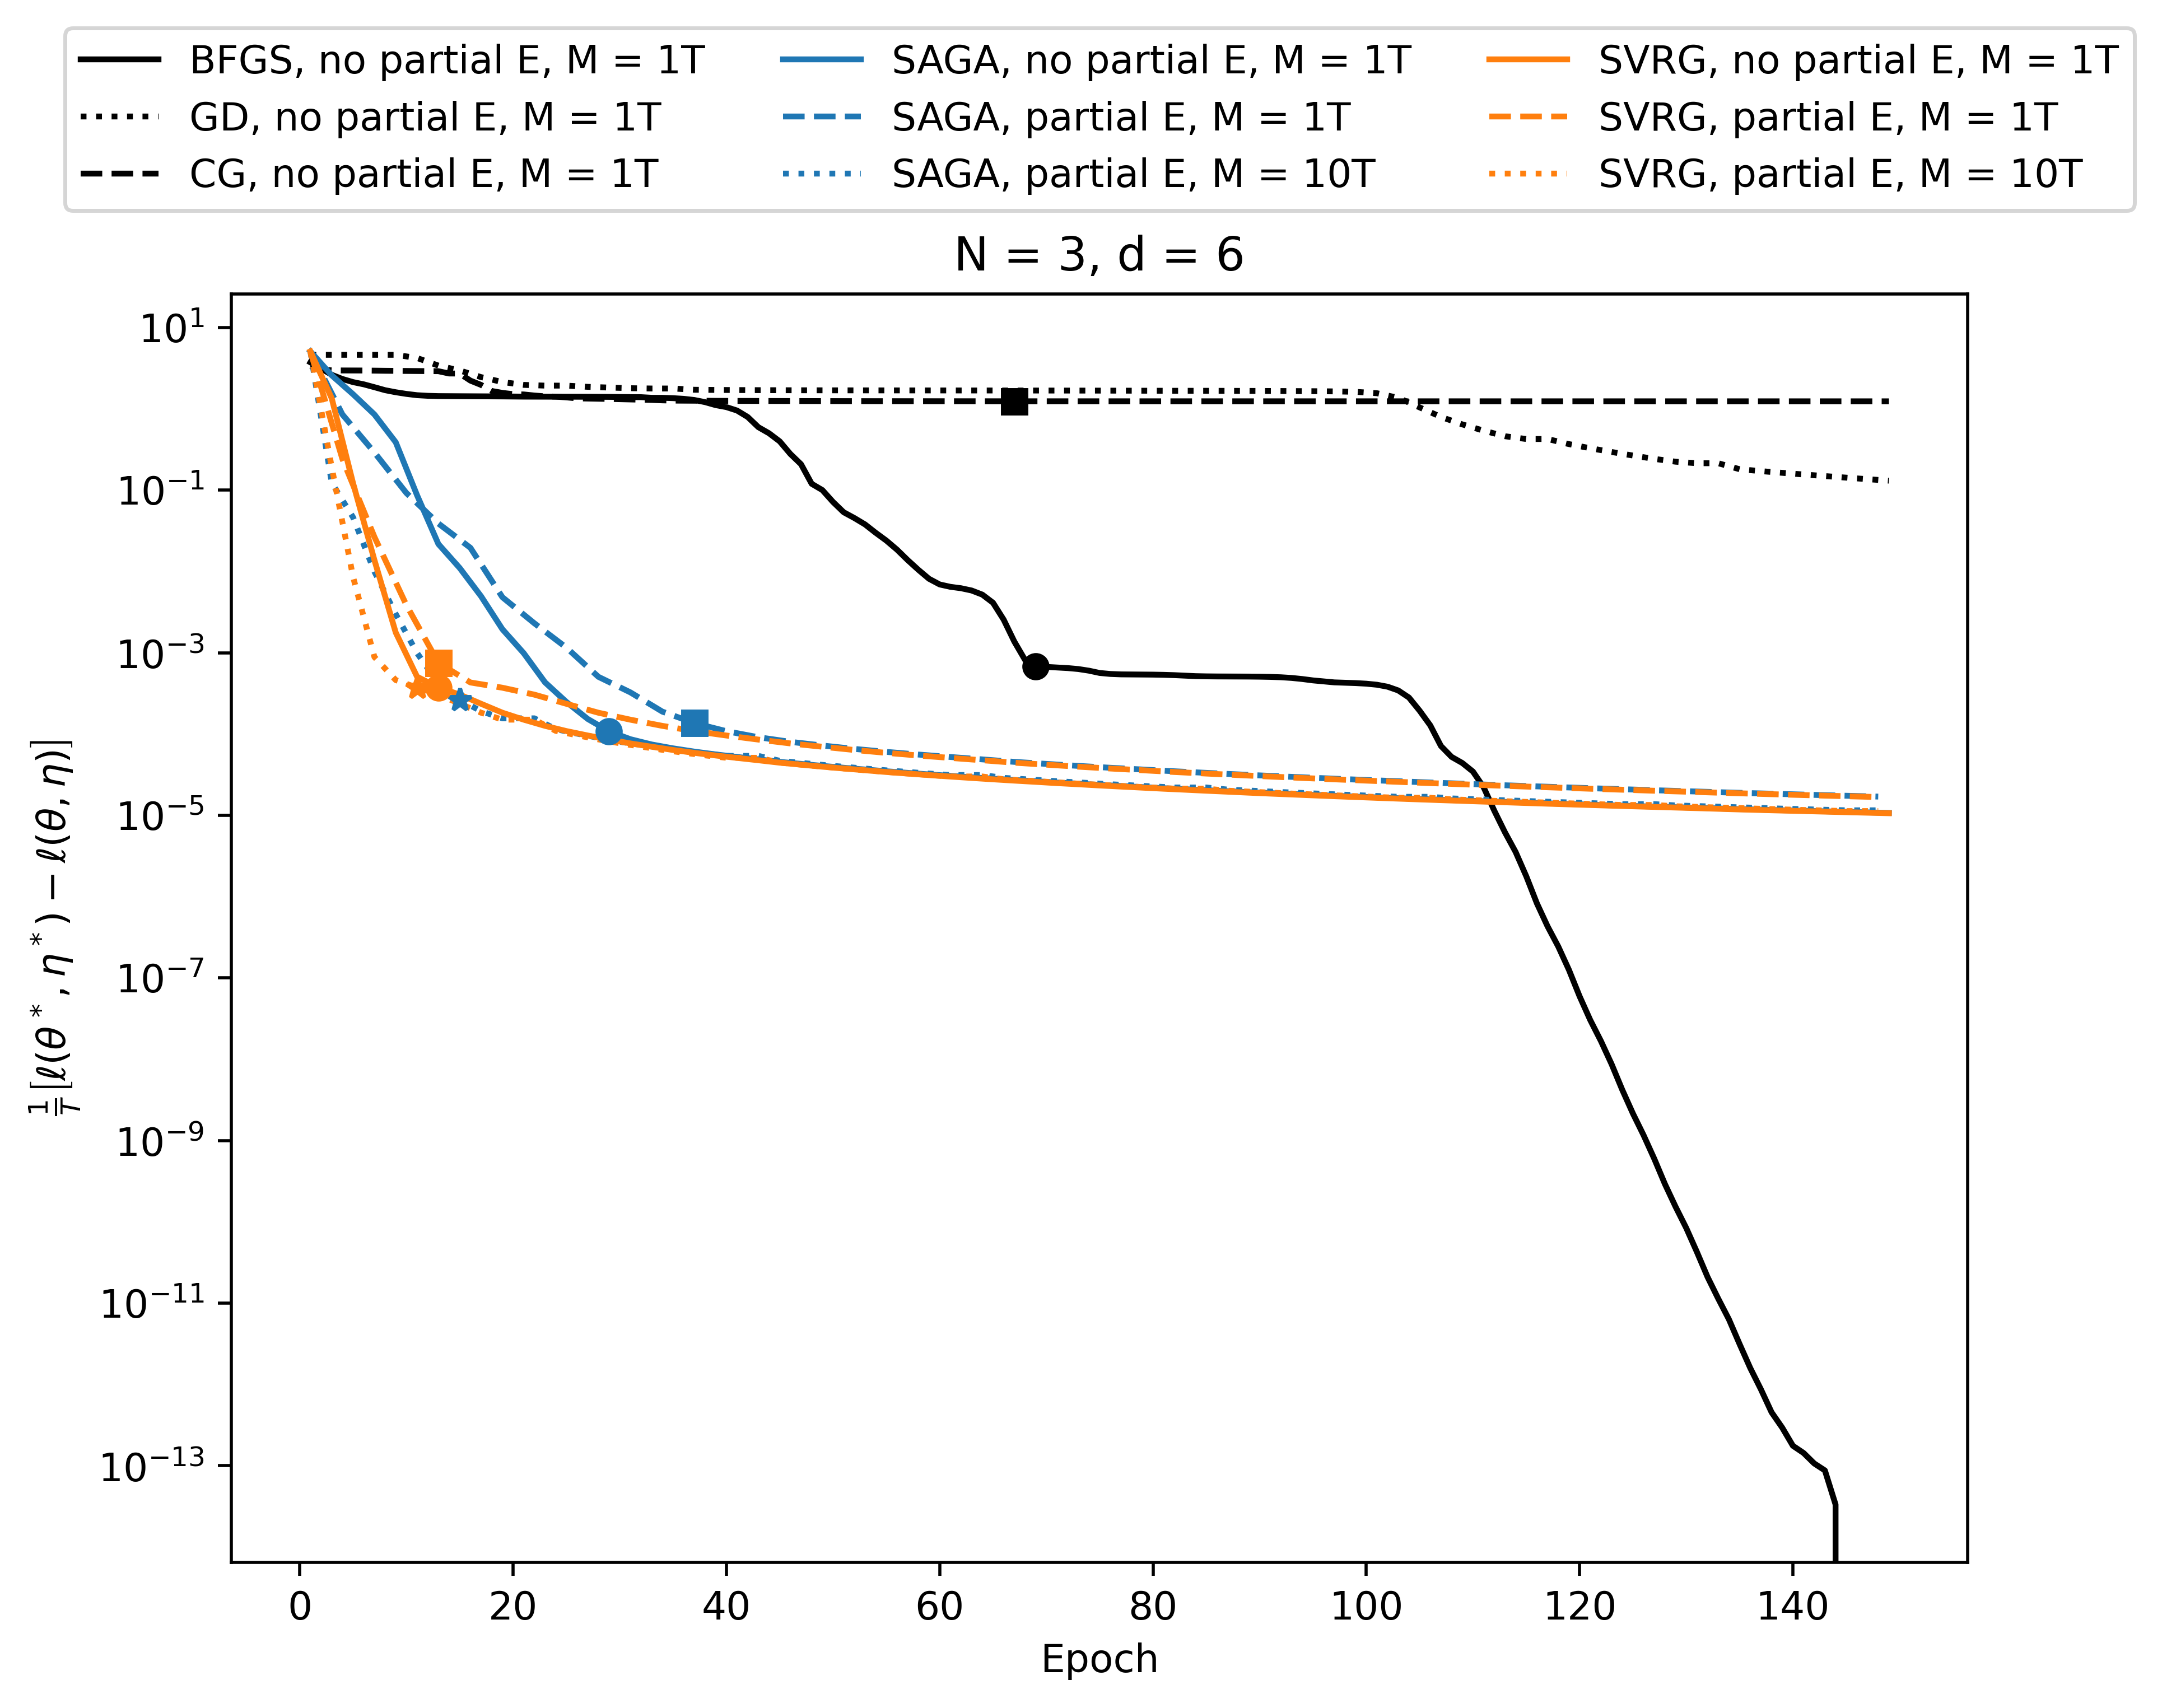
\includegraphics[width=3in]{../plt/log-like_v_epoch_T-1000-K-3-1-d-6-002.png}
    \\
    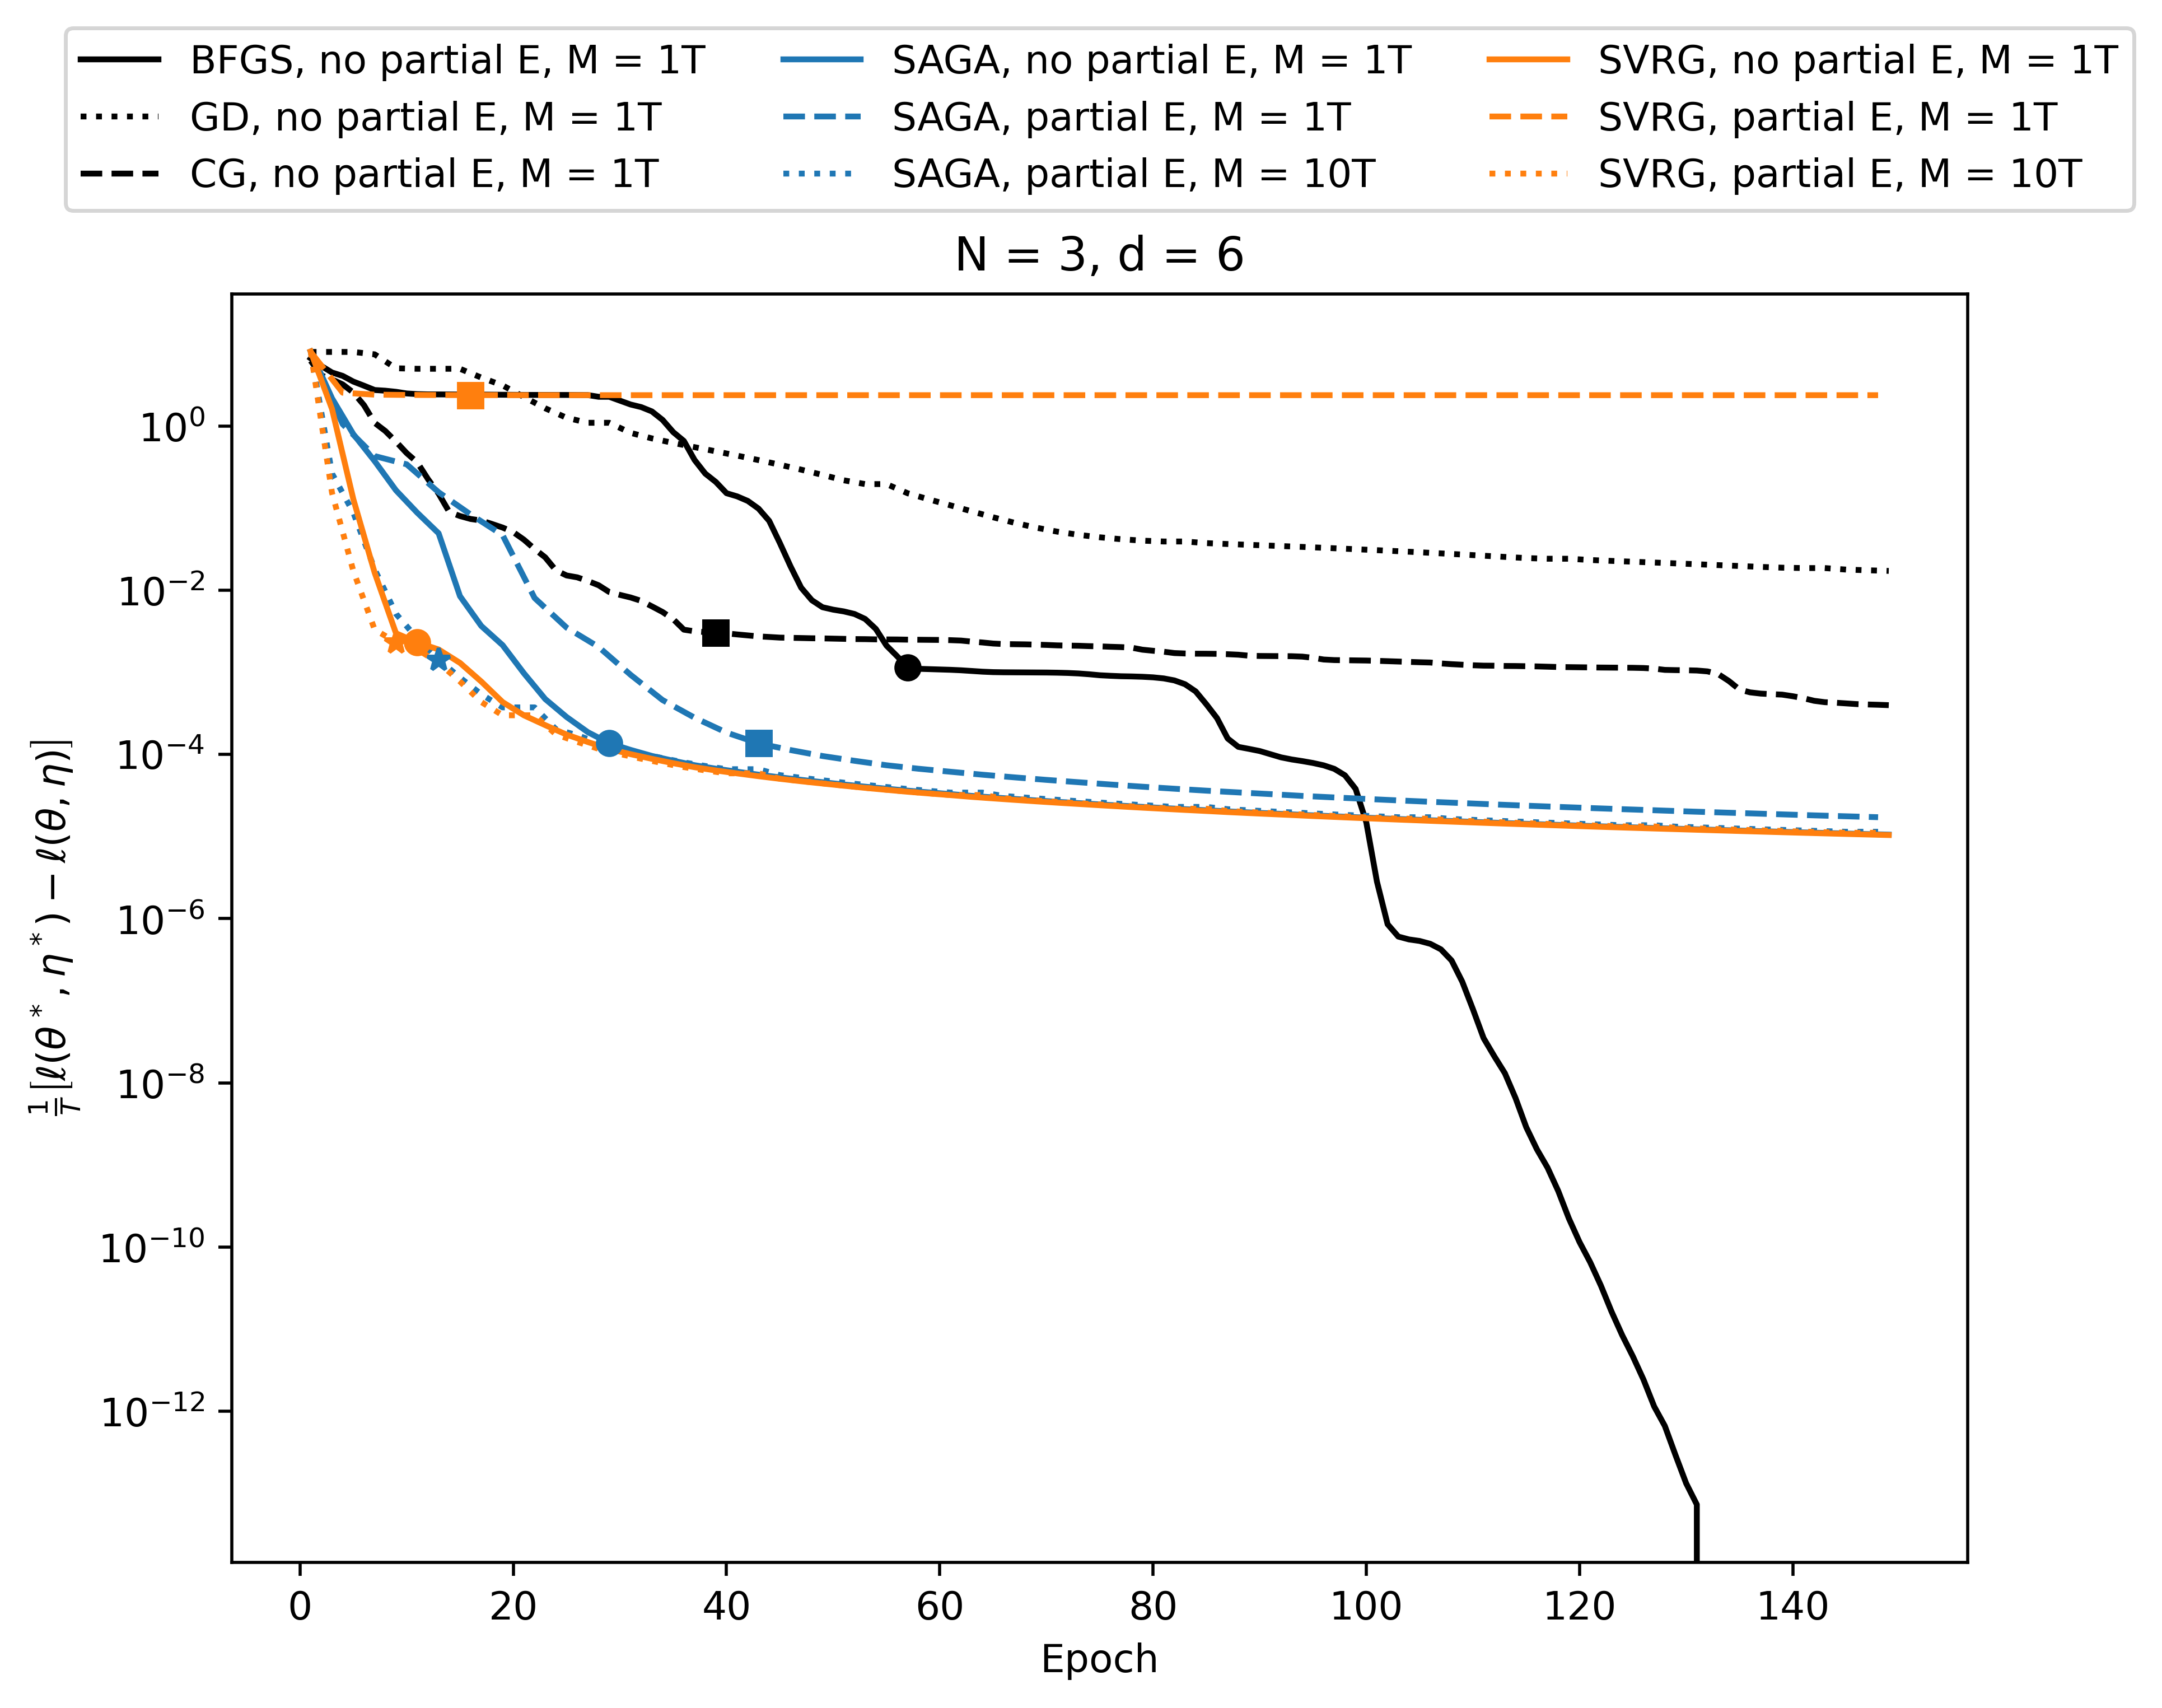
\includegraphics[width=3in]{../plt/log-like_v_epoch_T-1000-K-3-1-d-6-003.png}
    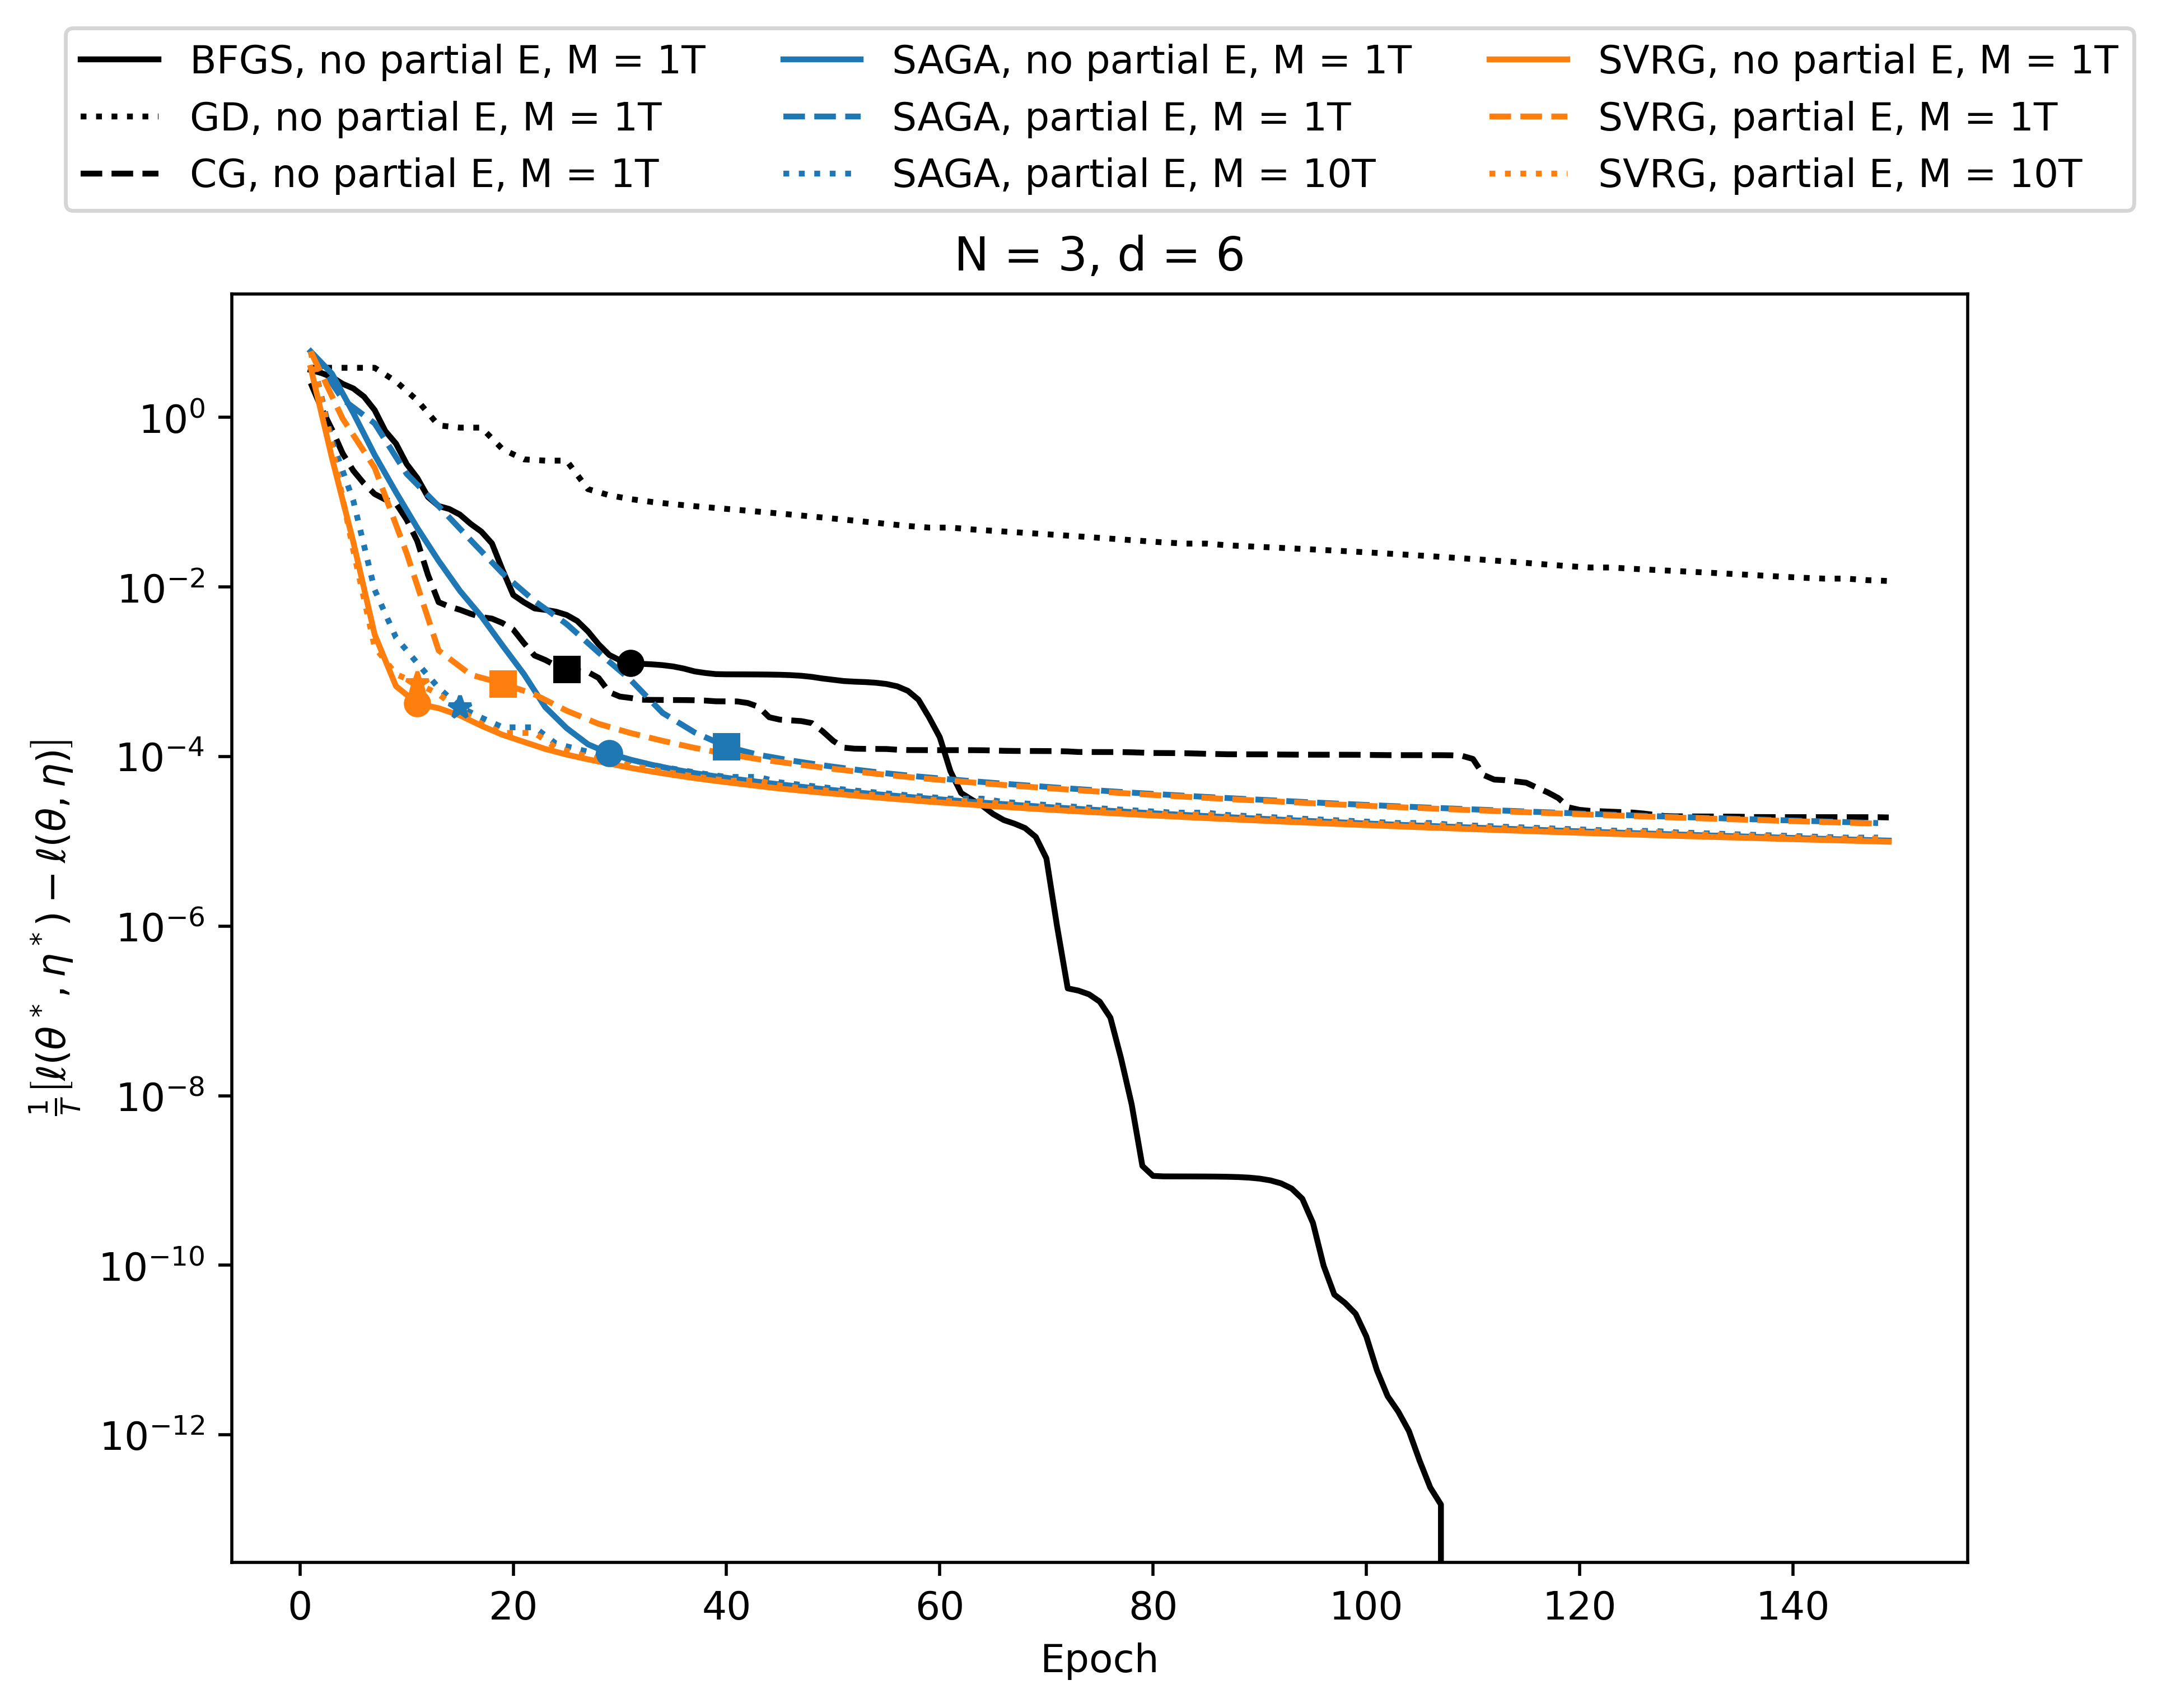
\includegraphics[width=3in]{../plt/log-like_v_epoch_T-1000-K-3-1-d-6-004.png}   
    \caption{Optimally gap between the current log-likelihood and optimal log-likelihood for the simulation studies with $T=10^{3}$, $N=3$ and $d=6$, for four different simulated data sets. One epoch represents either one full E-step, $T$ iterations with the M-step, or one gradient step for full-gradient algorithms. The y-axis is on a log-scale.}
\end{figure}
%
\begin{figure}
    \centering
    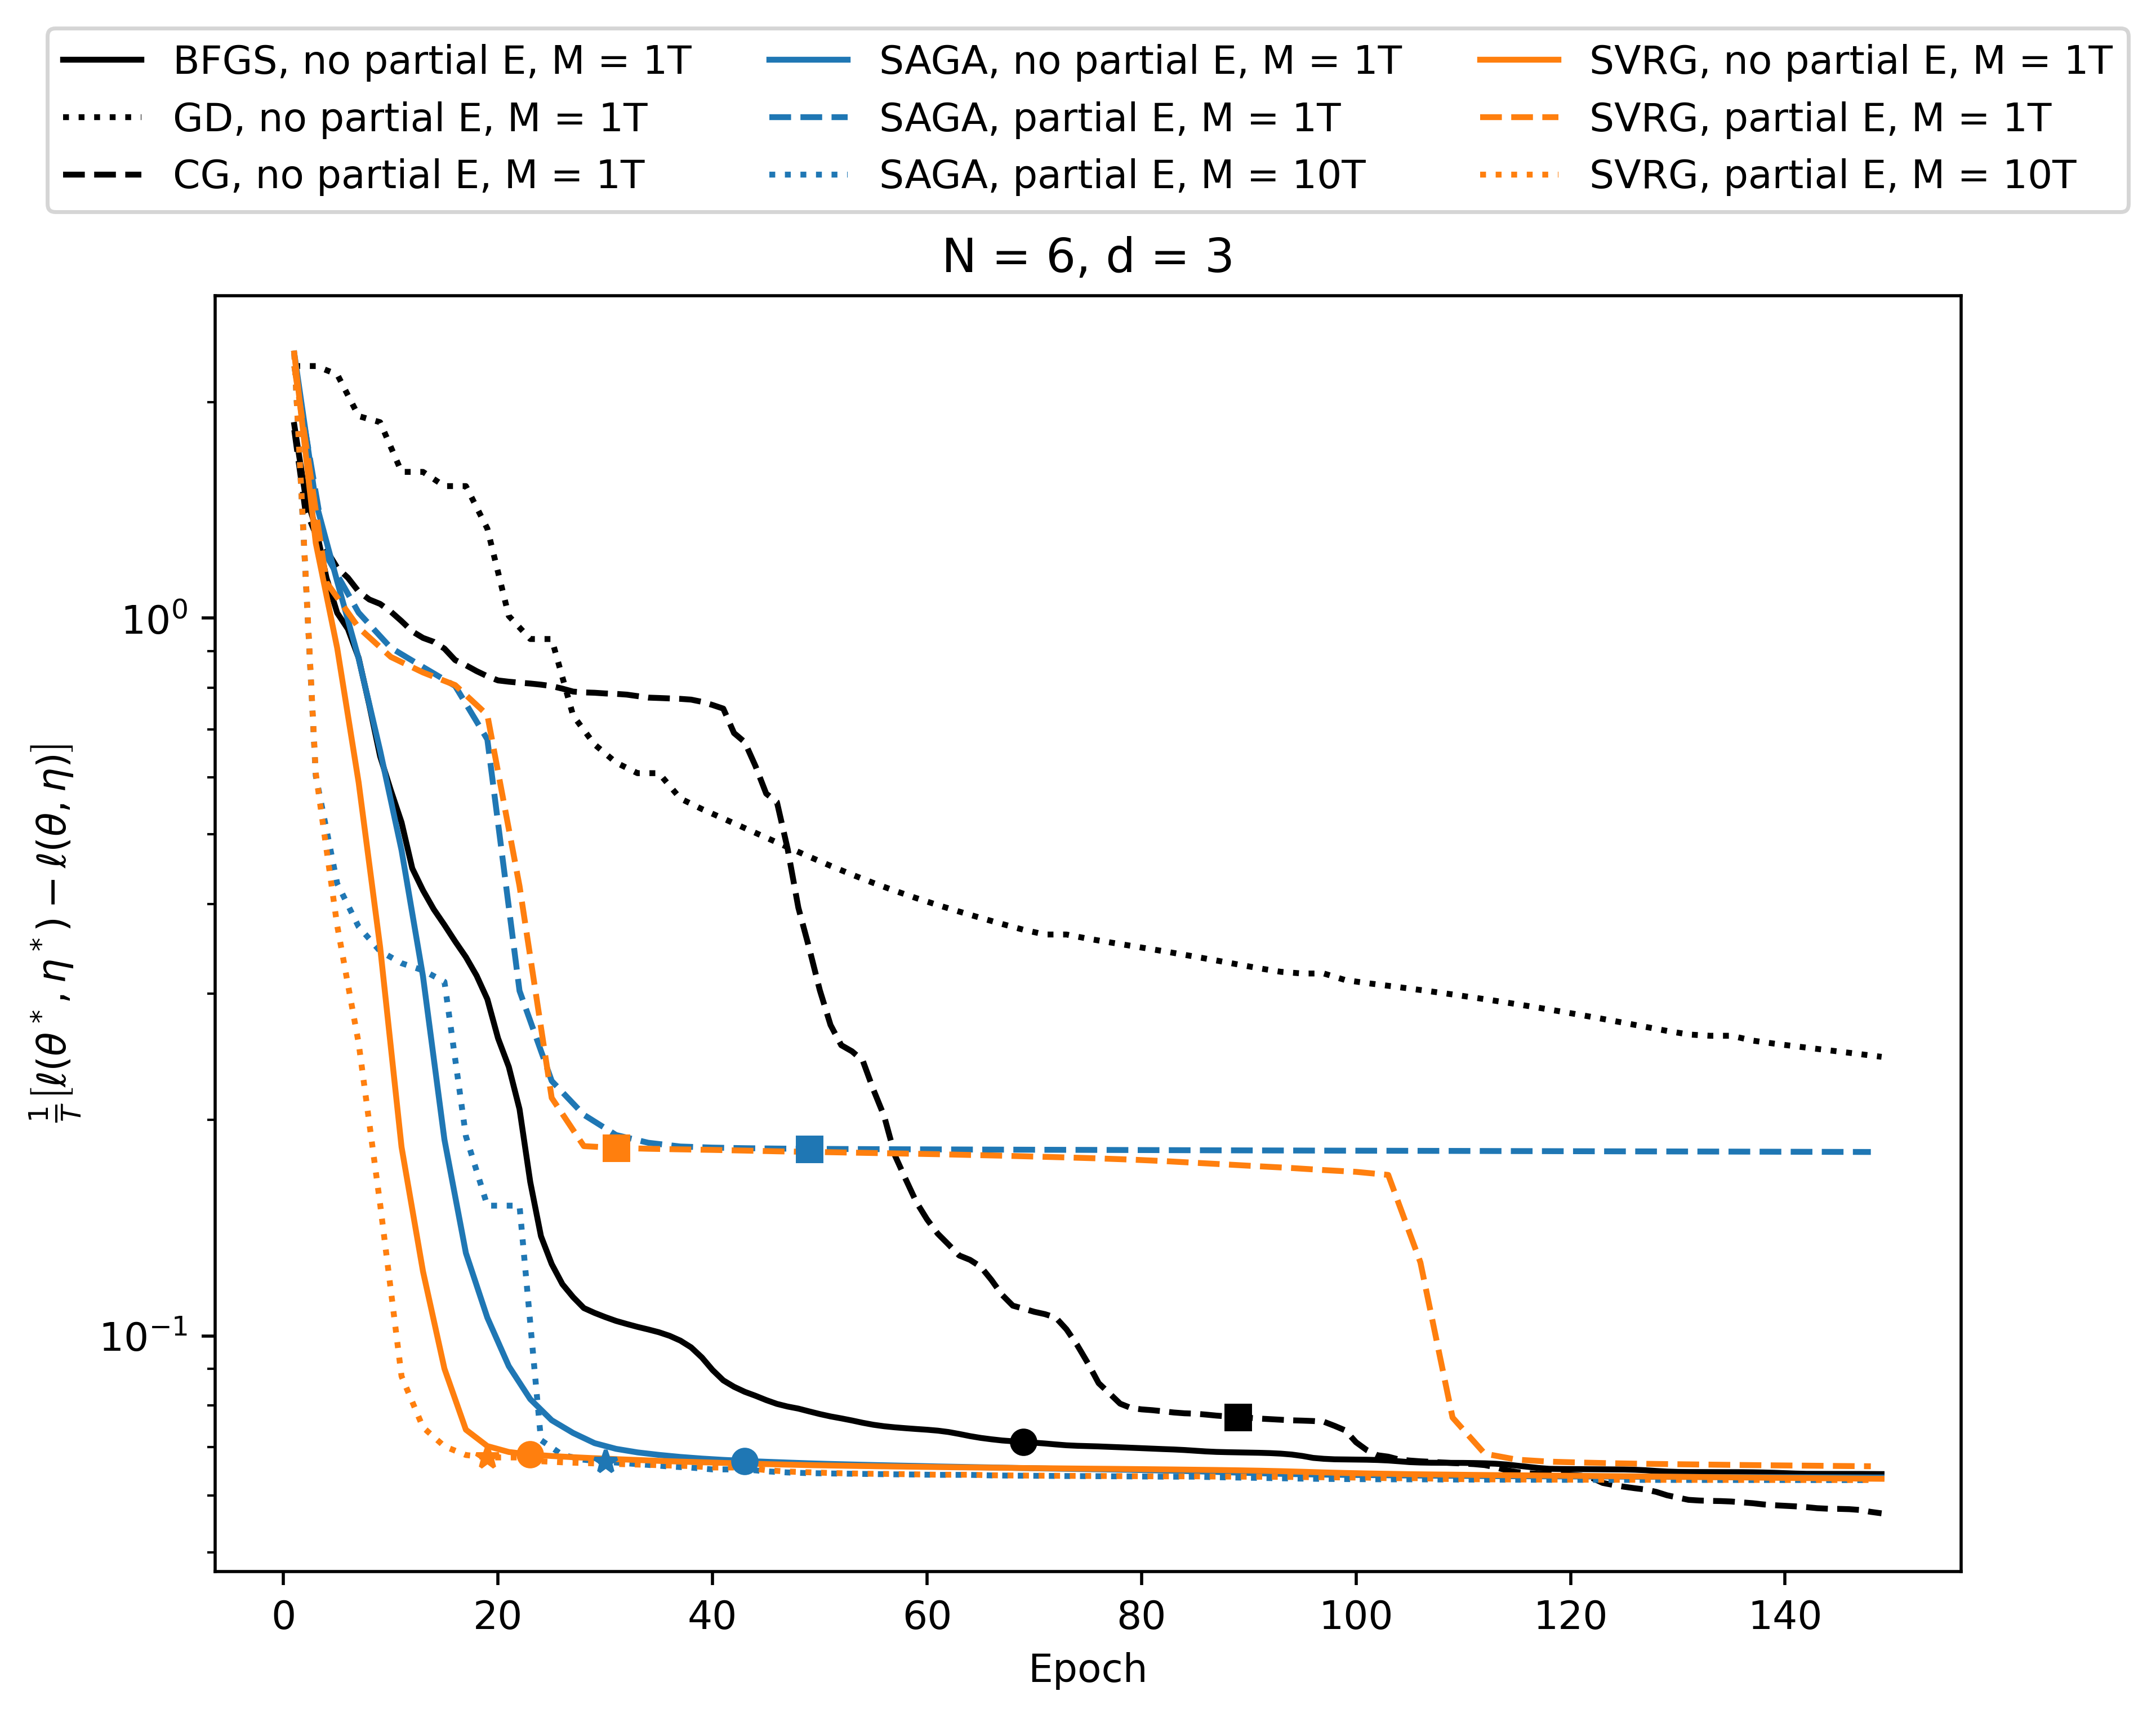
\includegraphics[width=3in]{../plt/log-like_v_epoch_T-1000-K-6-1-d-3-001.png}
    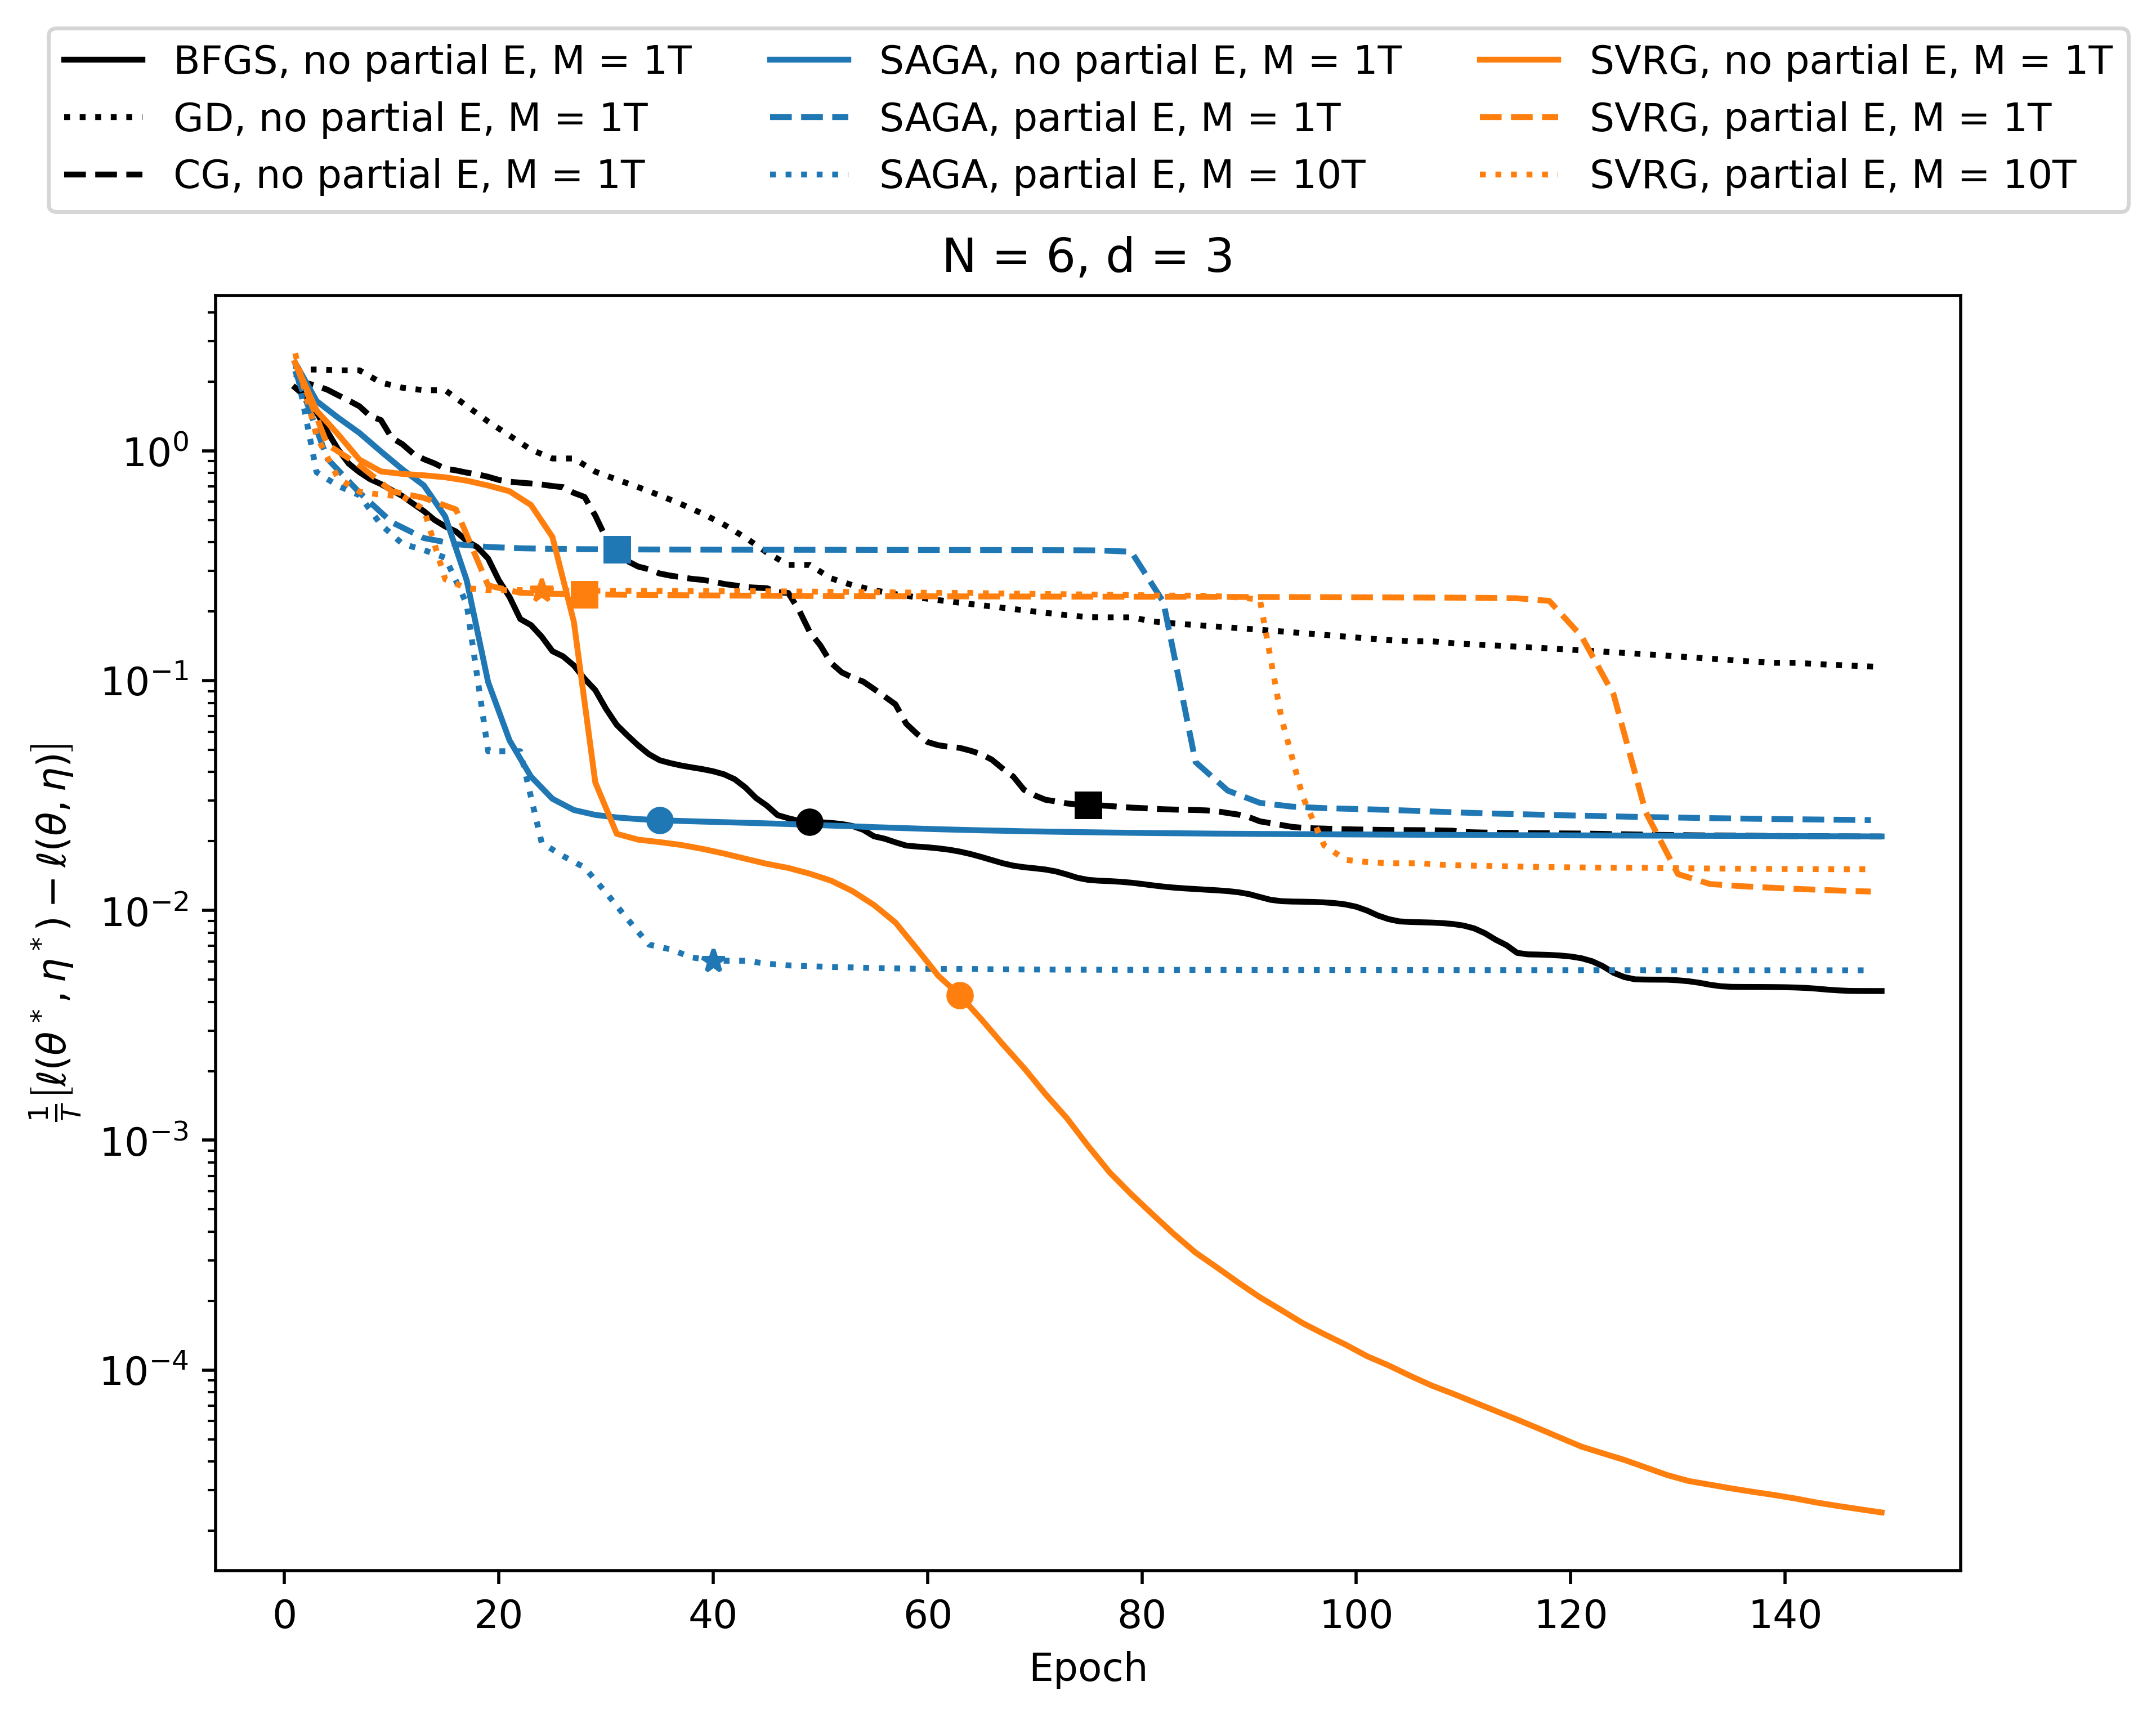
\includegraphics[width=3in]{../plt/log-like_v_epoch_T-1000-K-6-1-d-3-002.png}
    \\
    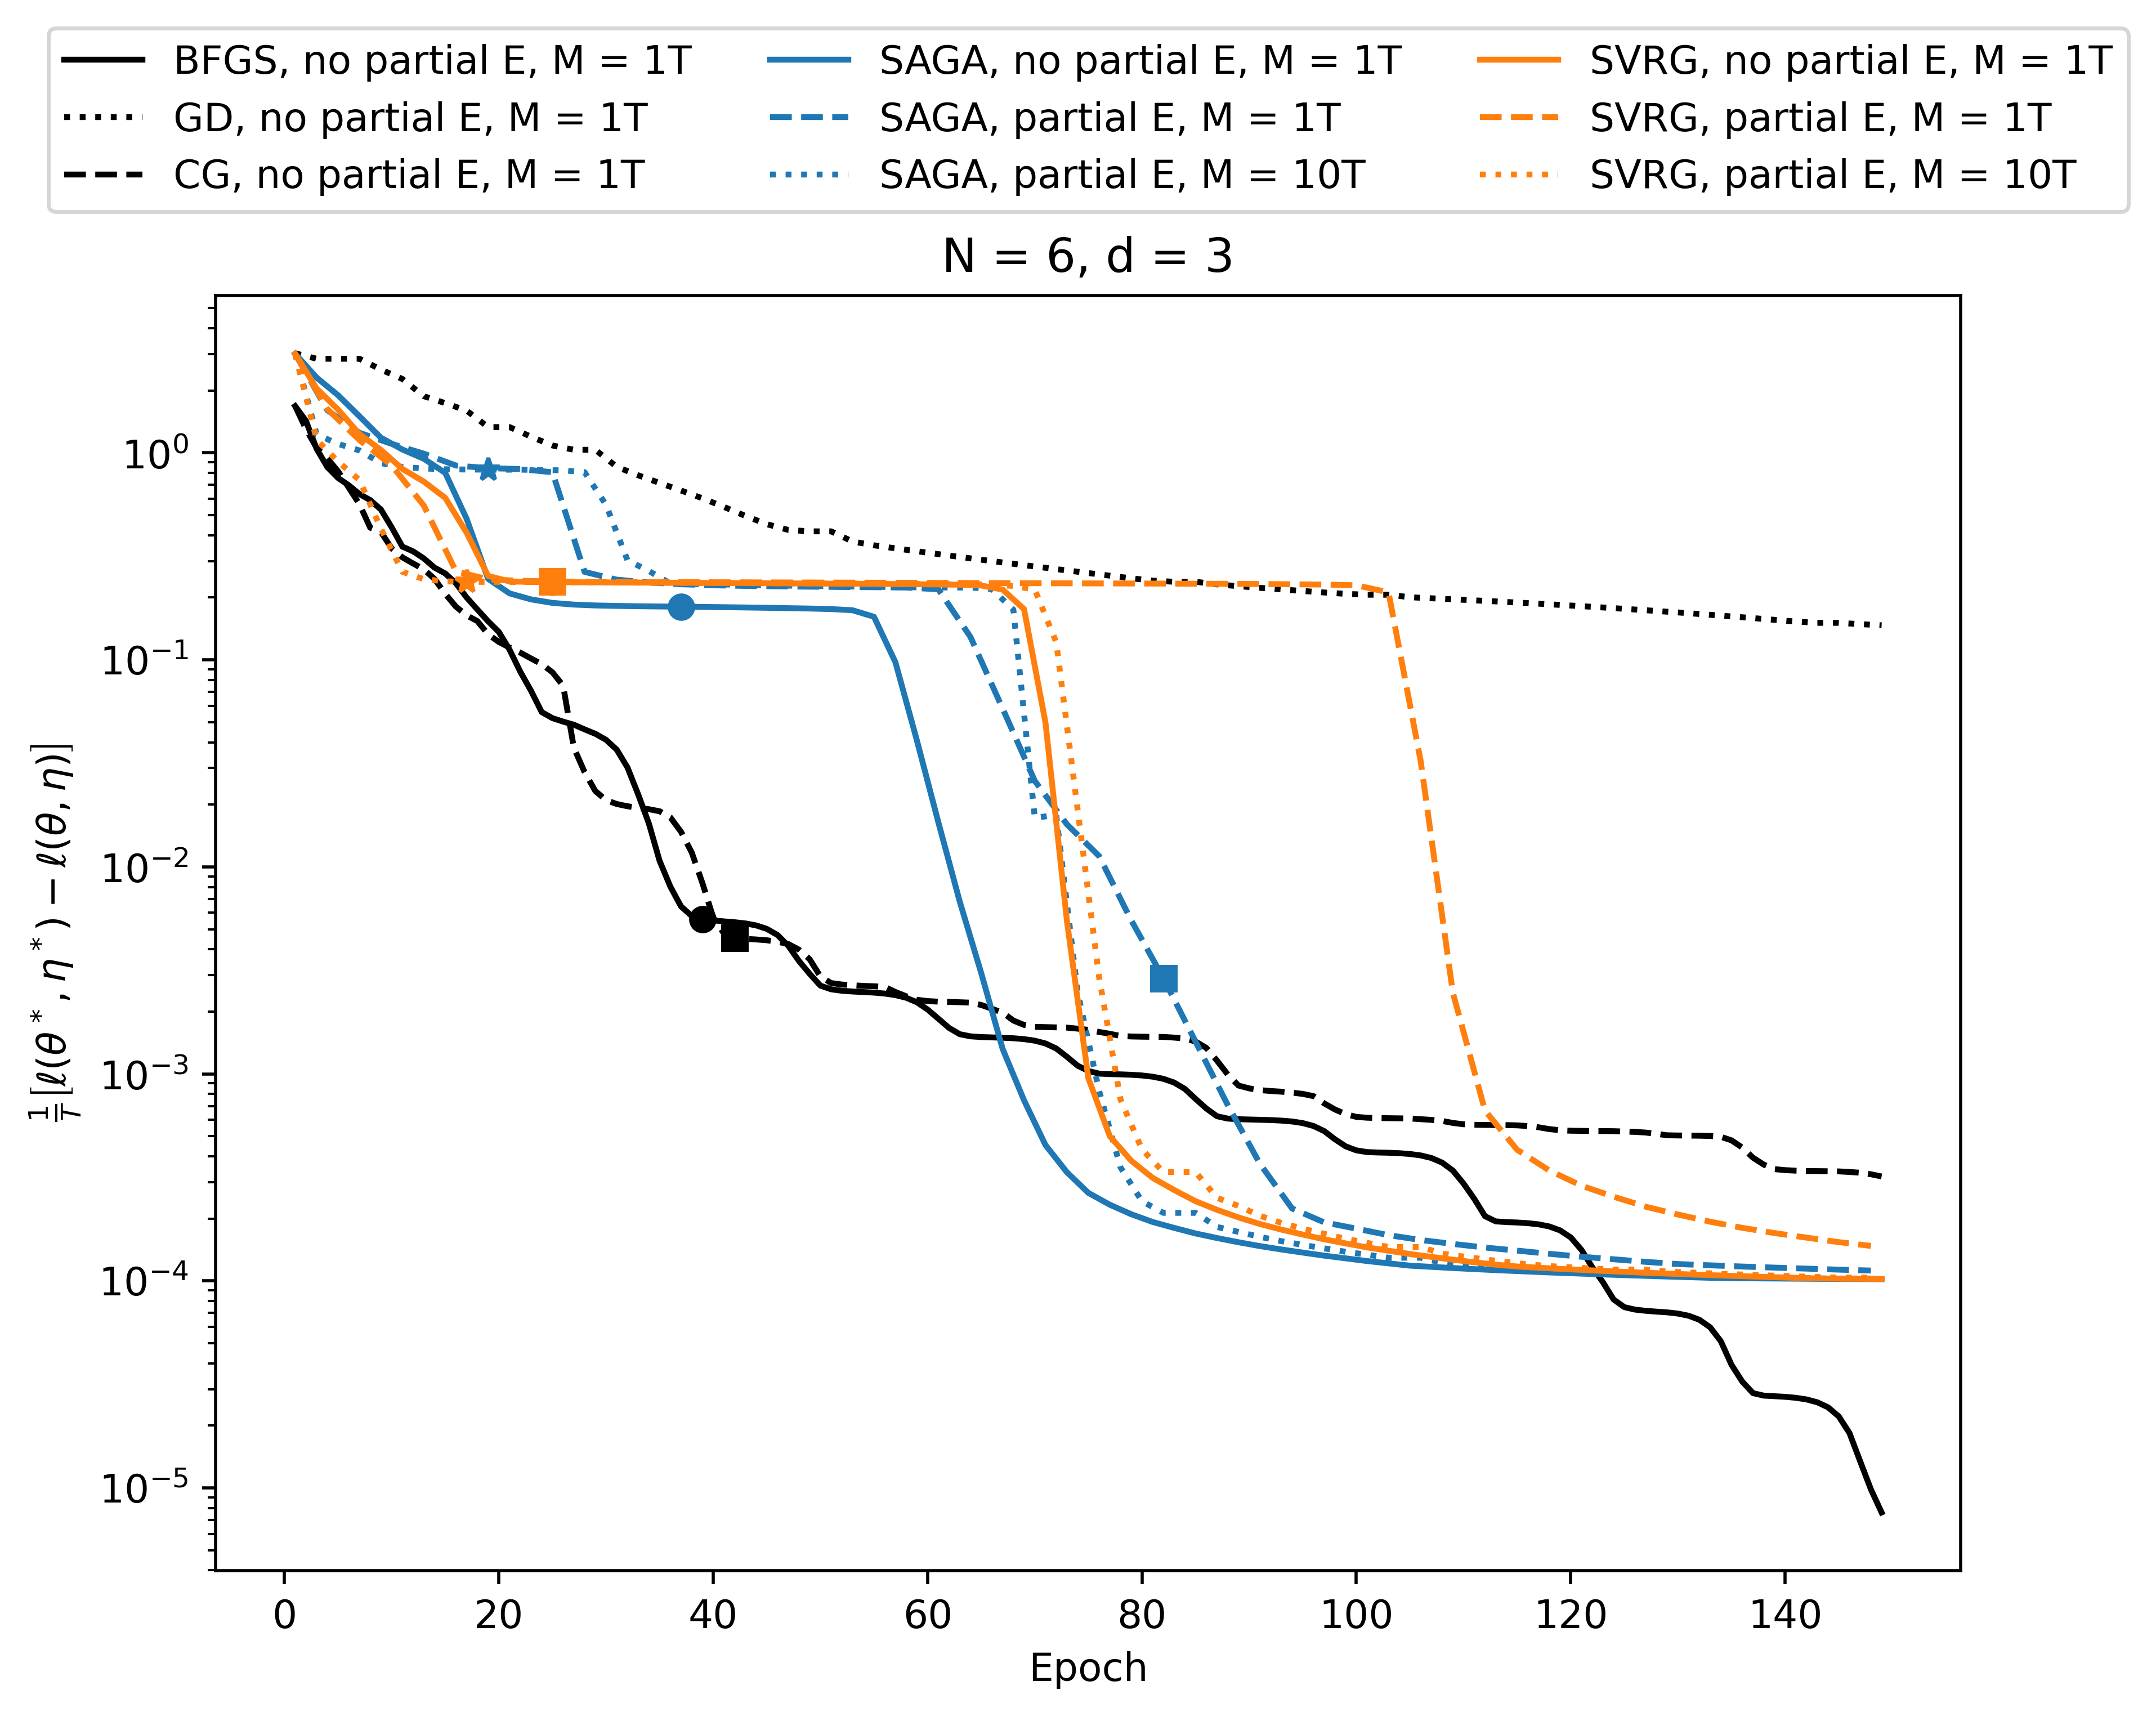
\includegraphics[width=3in]{../plt/log-like_v_epoch_T-1000-K-6-1-d-3-003.png}
    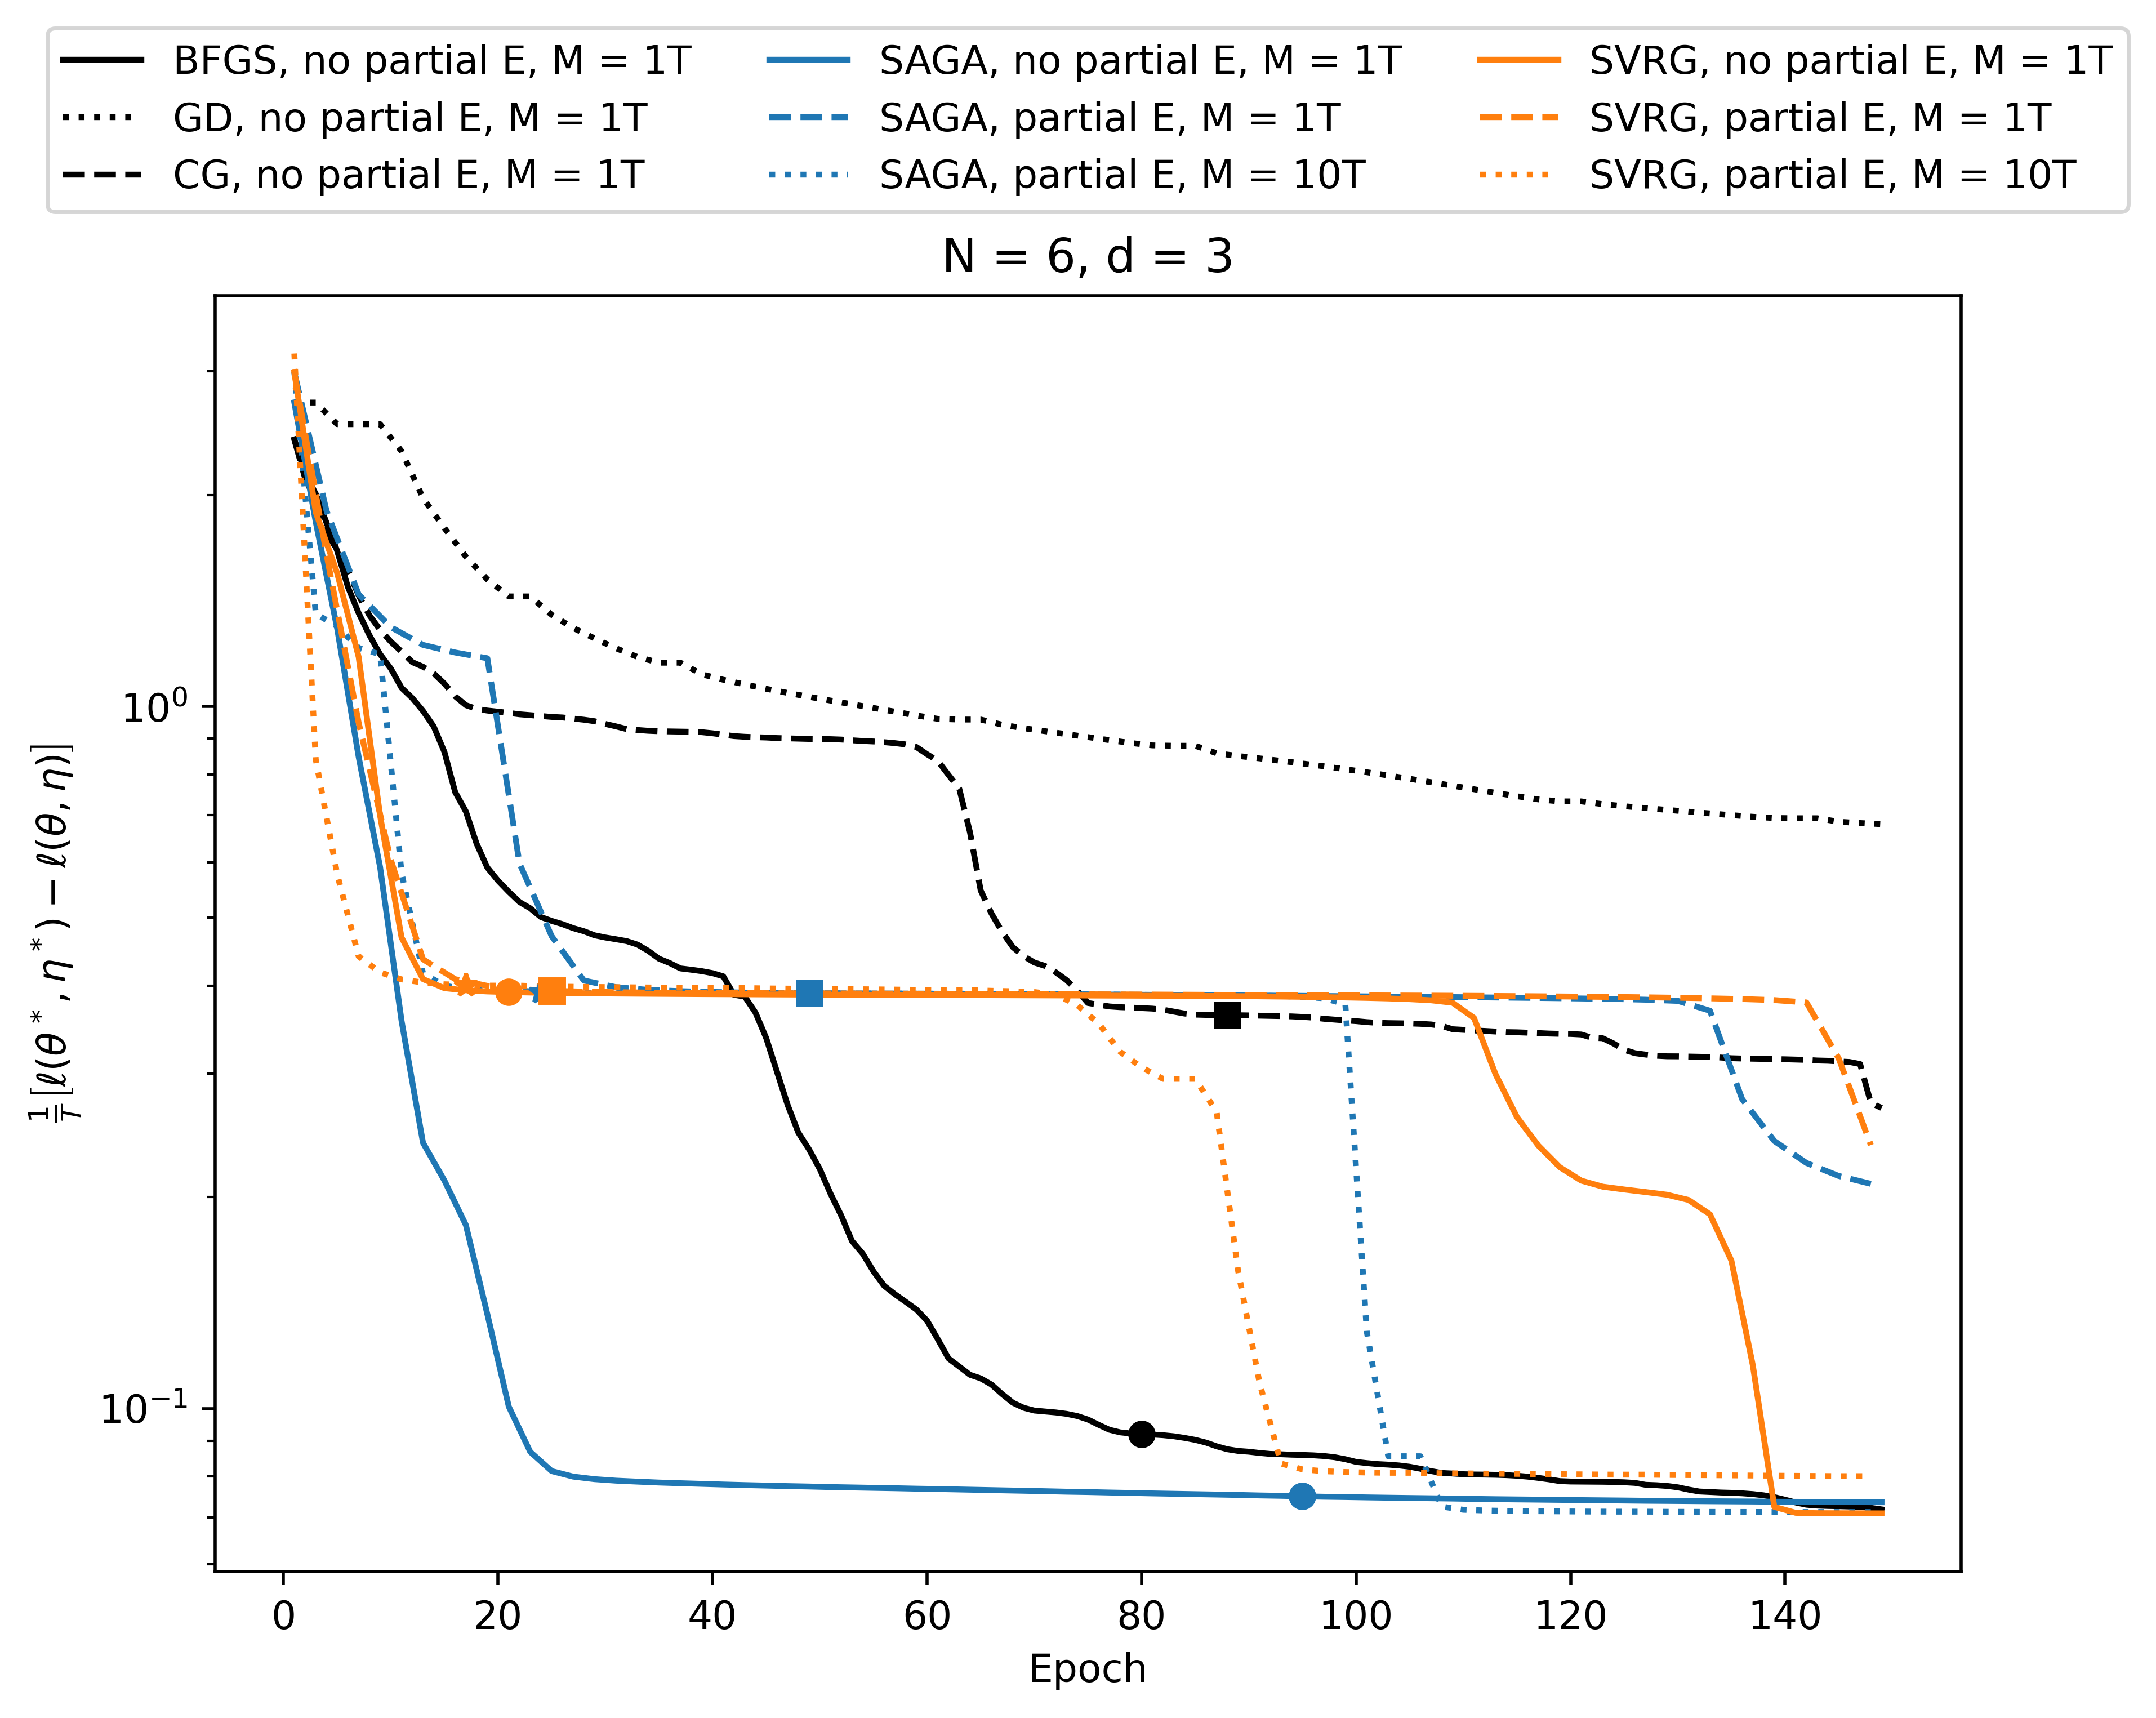
\includegraphics[width=3in]{../plt/log-like_v_epoch_T-1000-K-6-1-d-3-004.png}   
    \caption{Optimally gap between the current log-likelihood and optimal log-likelihood for the simulation studies with $T=10^{3}$, $N=6$ and $d=3$, for four different simulated data sets. One epoch represents either one full E-step, $T$ iterations with the M-step, or one gradient step for full-gradient algorithms. The y-axis is on a log-scale.}
\end{figure}
%
\begin{figure}
    \centering
    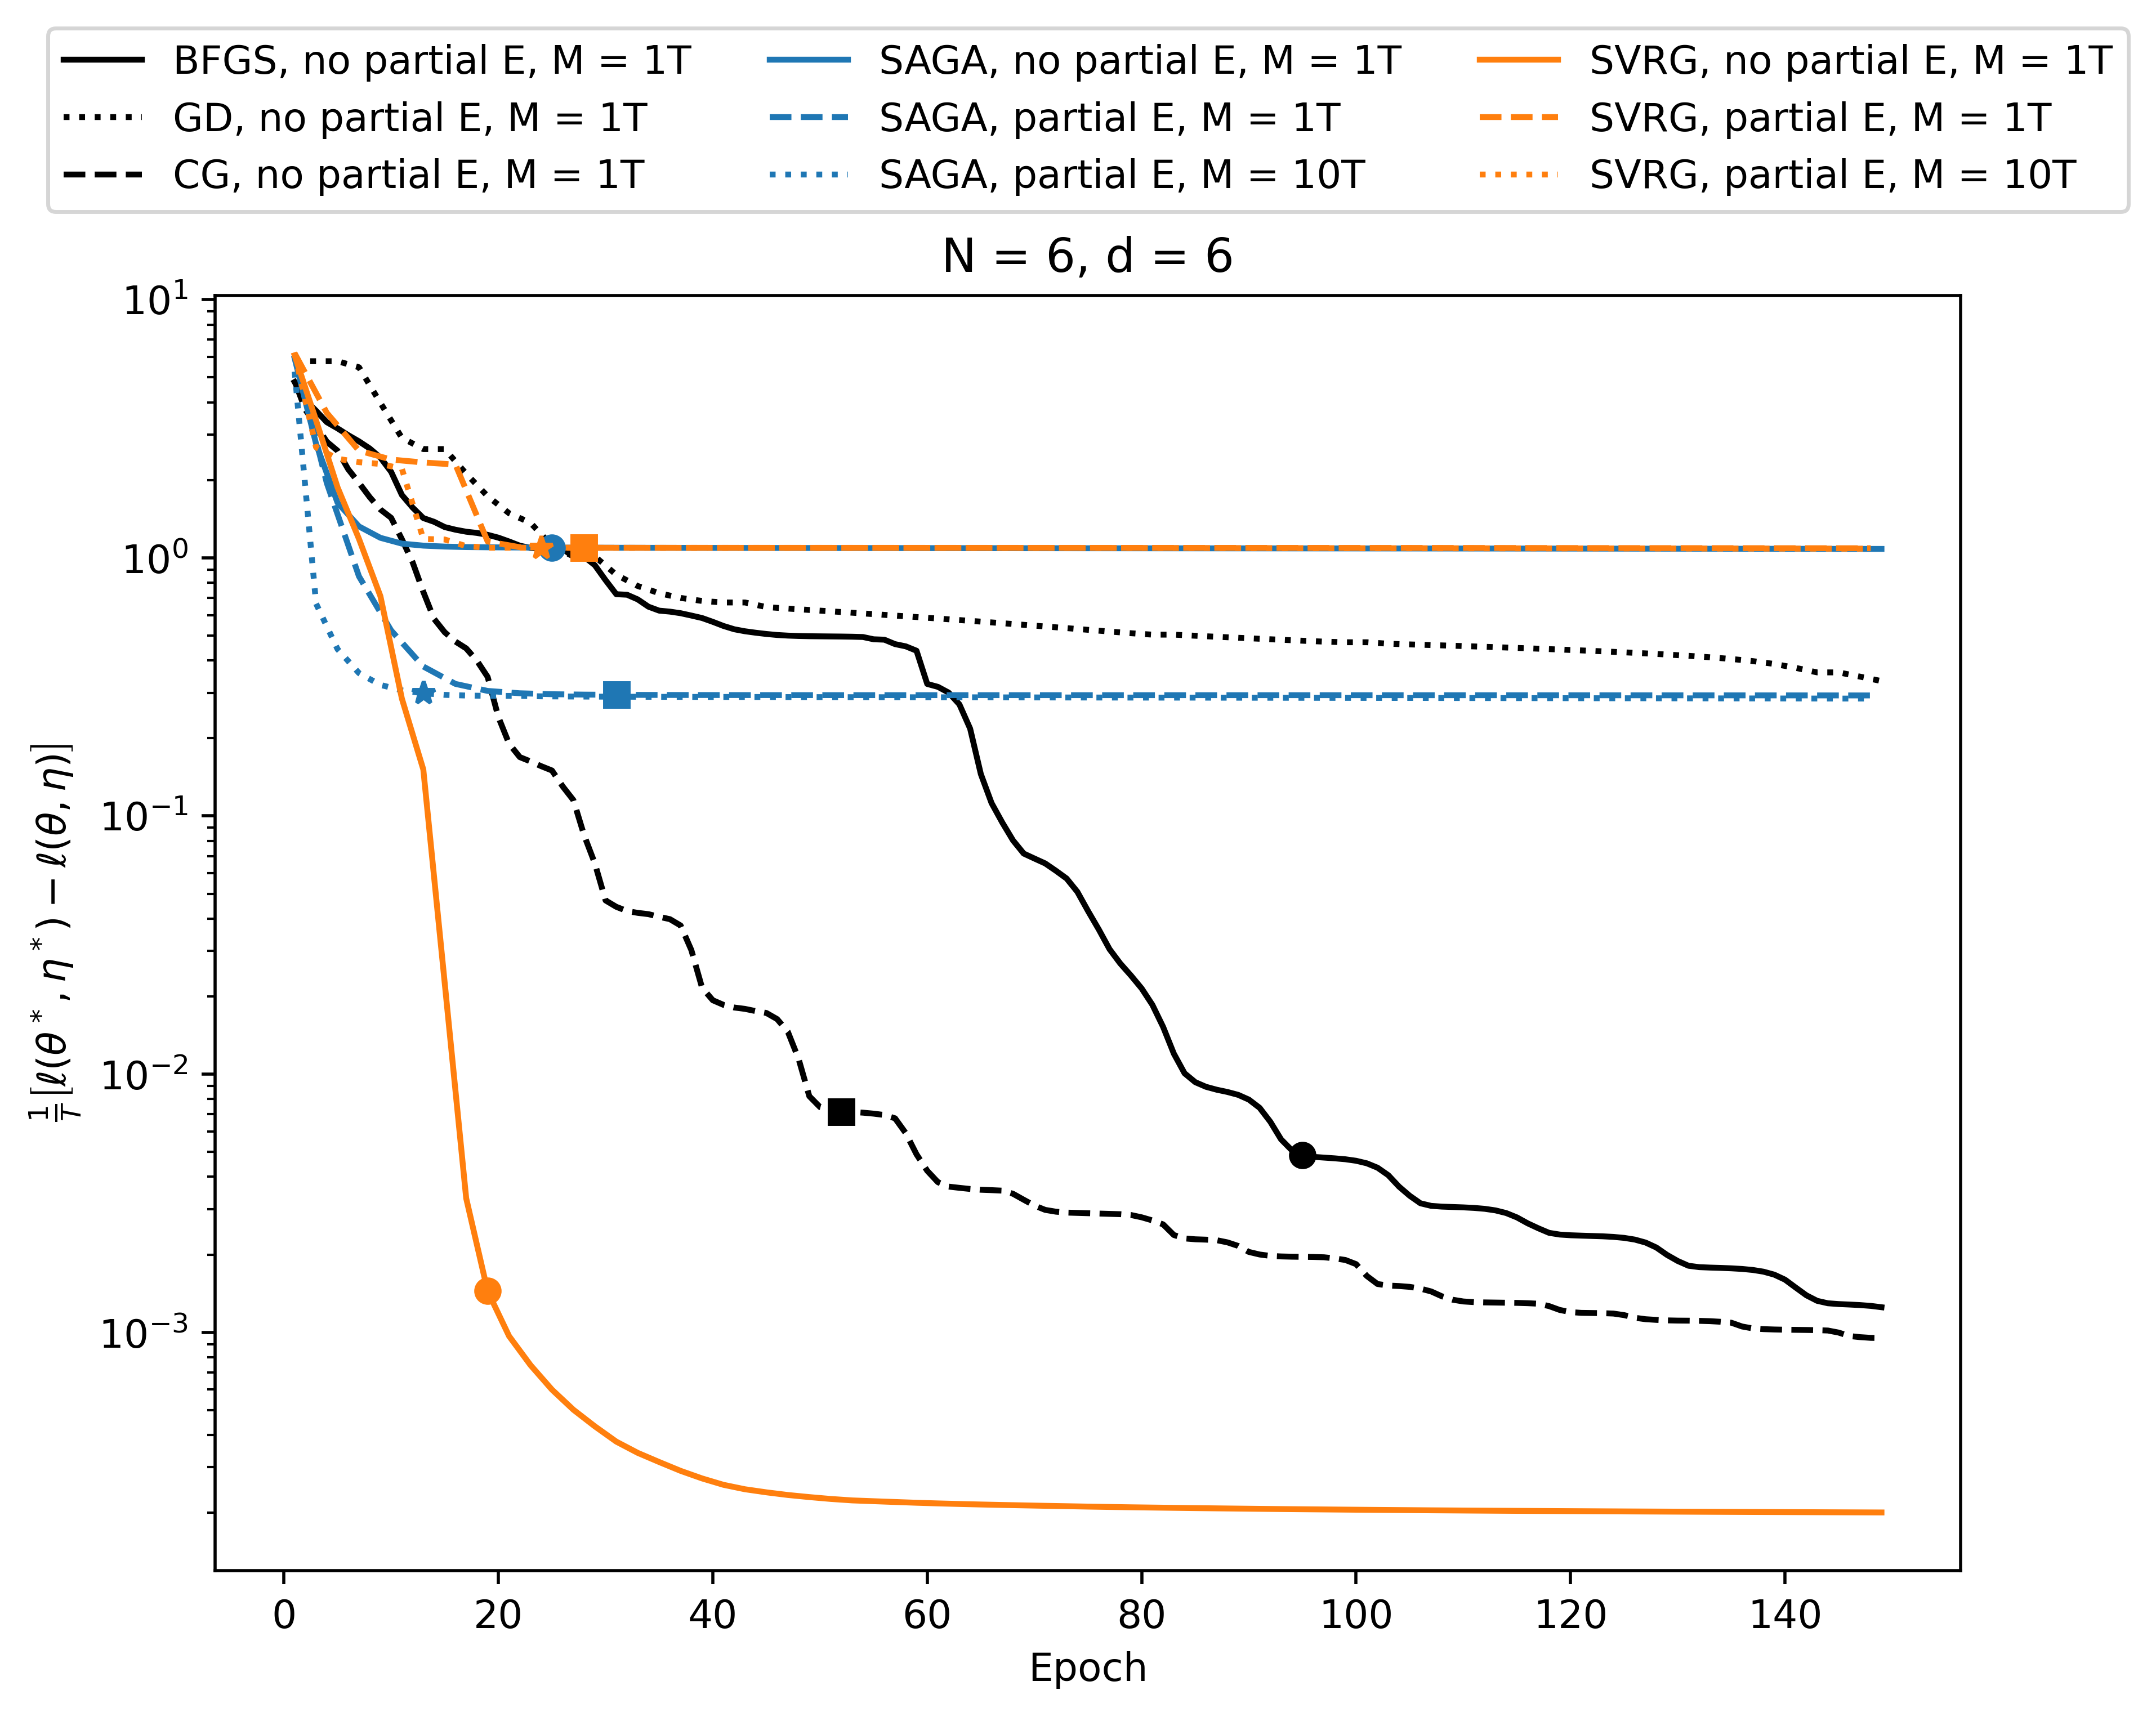
\includegraphics[width=3in]{../plt/log-like_v_epoch_T-1000-K-6-1-d-6-001.png}
    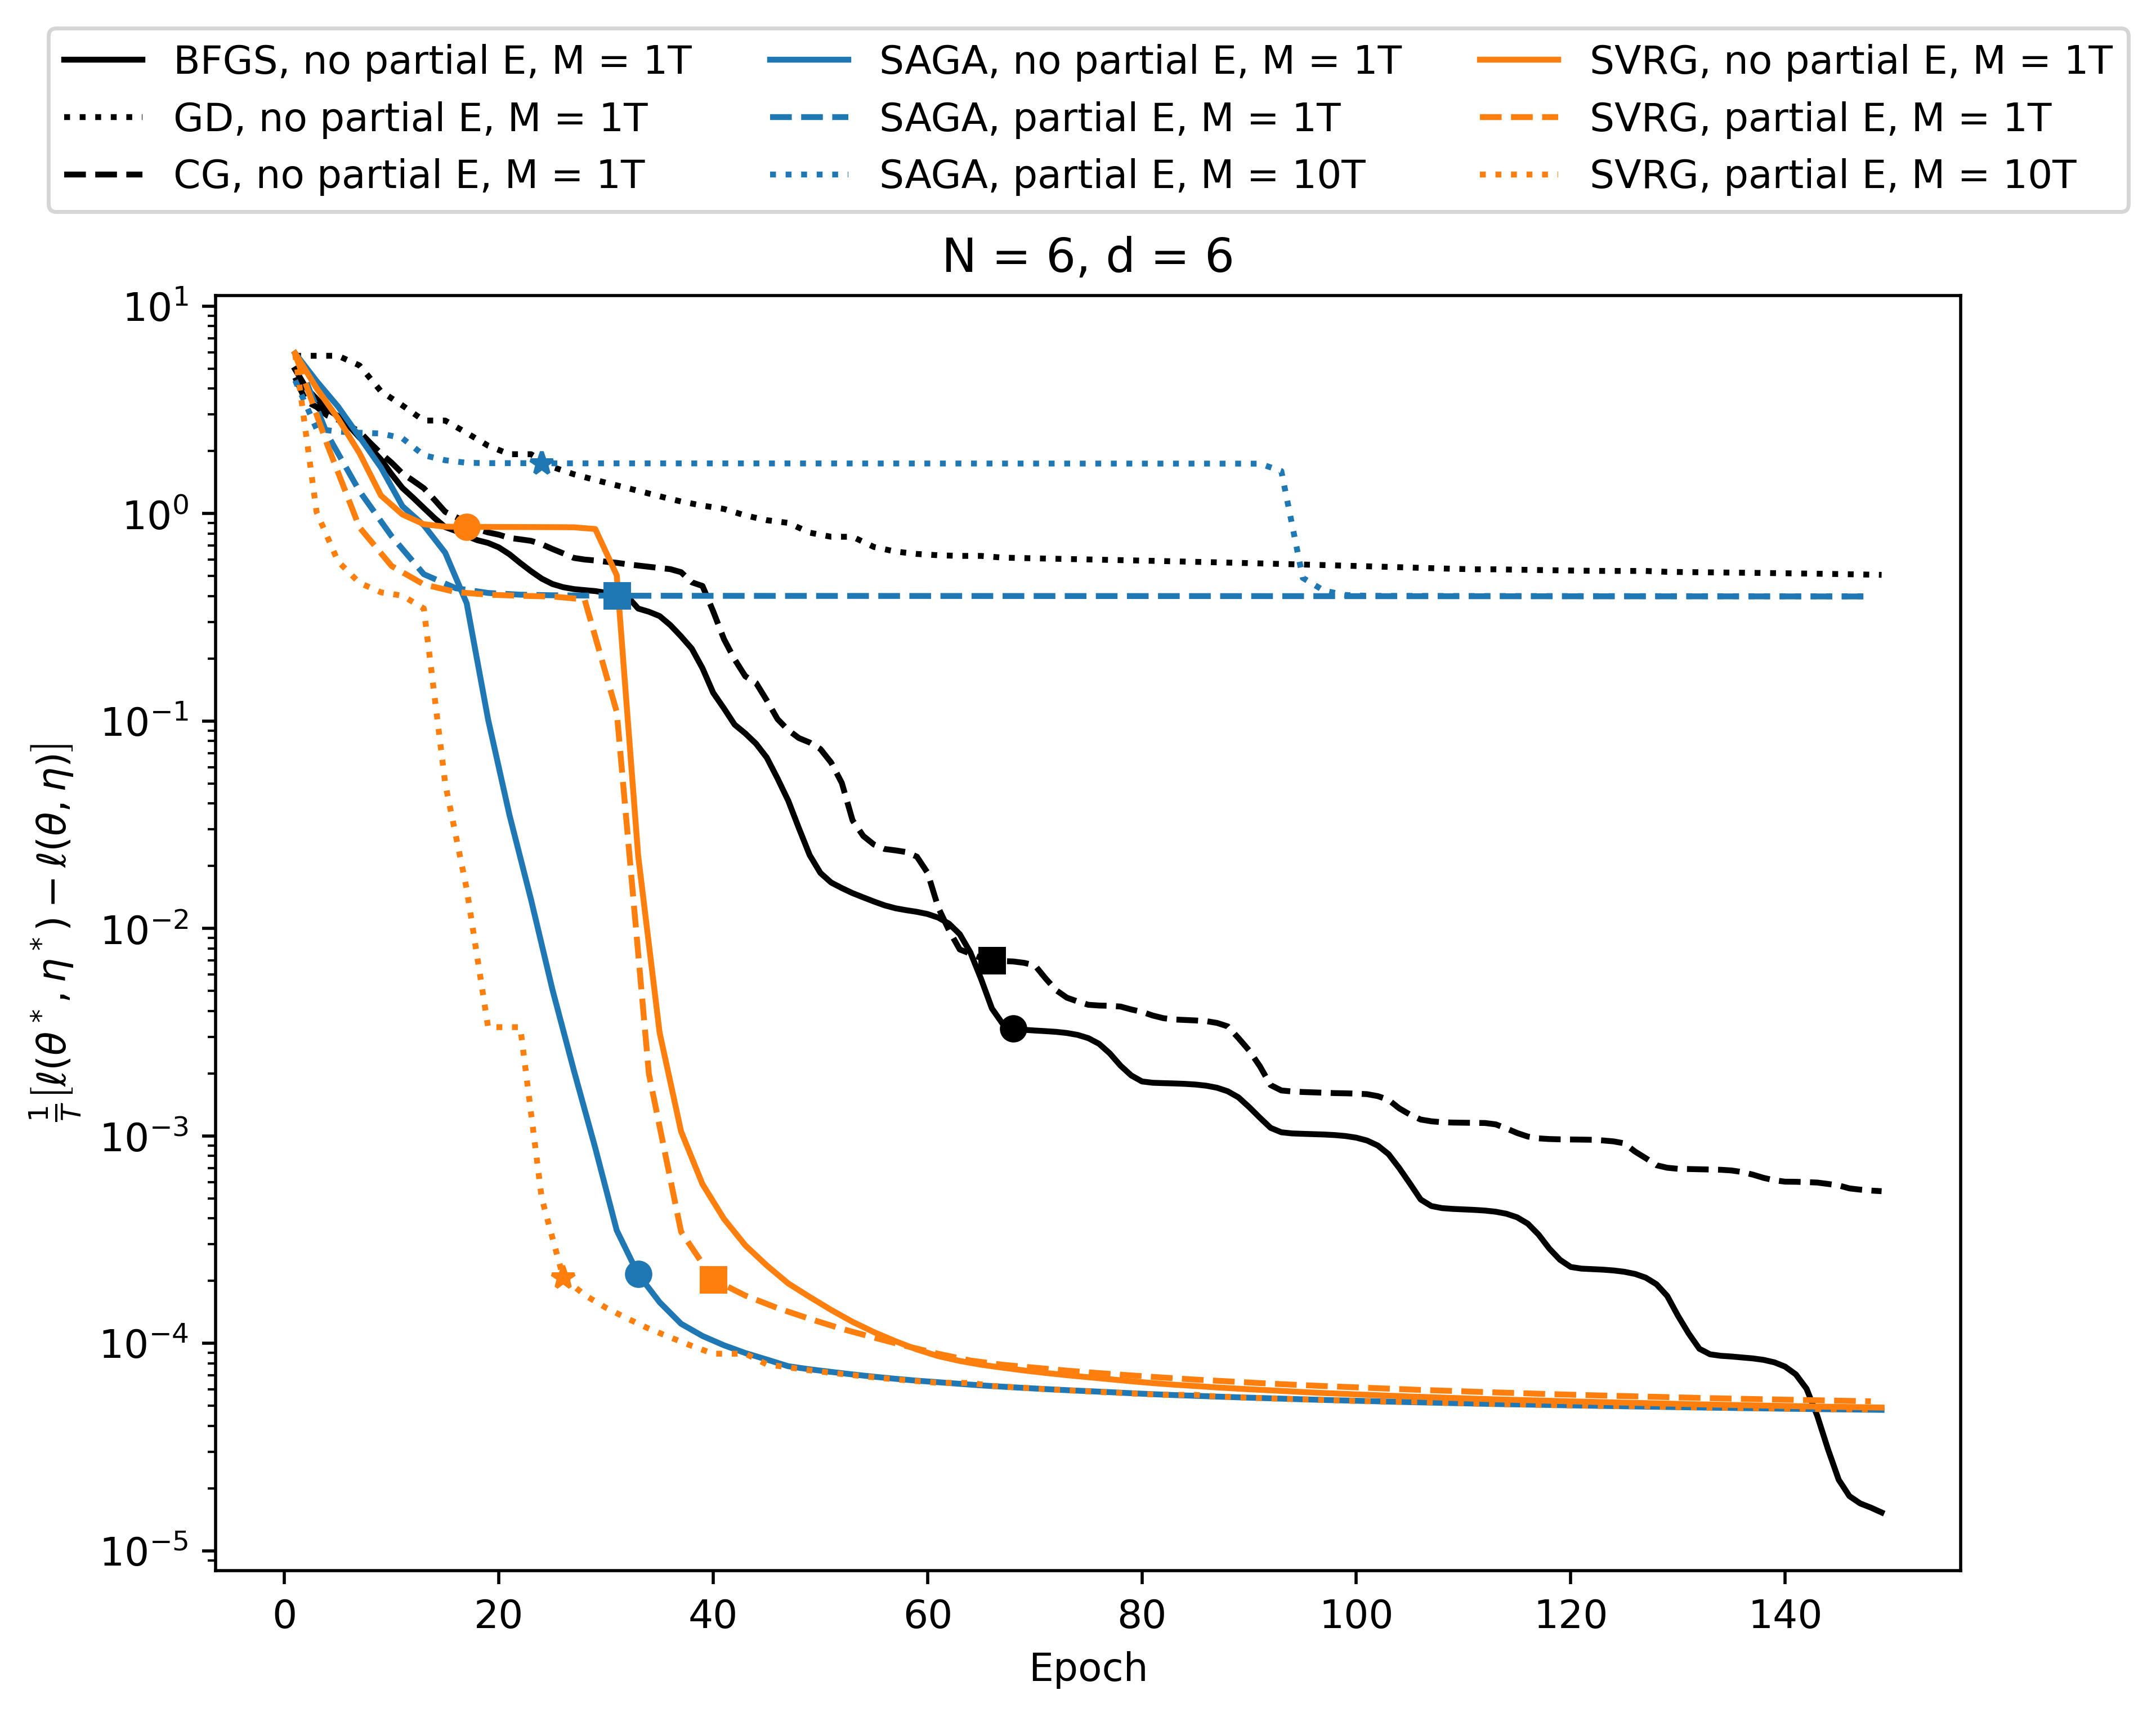
\includegraphics[width=3in]{../plt/log-like_v_epoch_T-1000-K-6-1-d-6-002.png}
    \\
    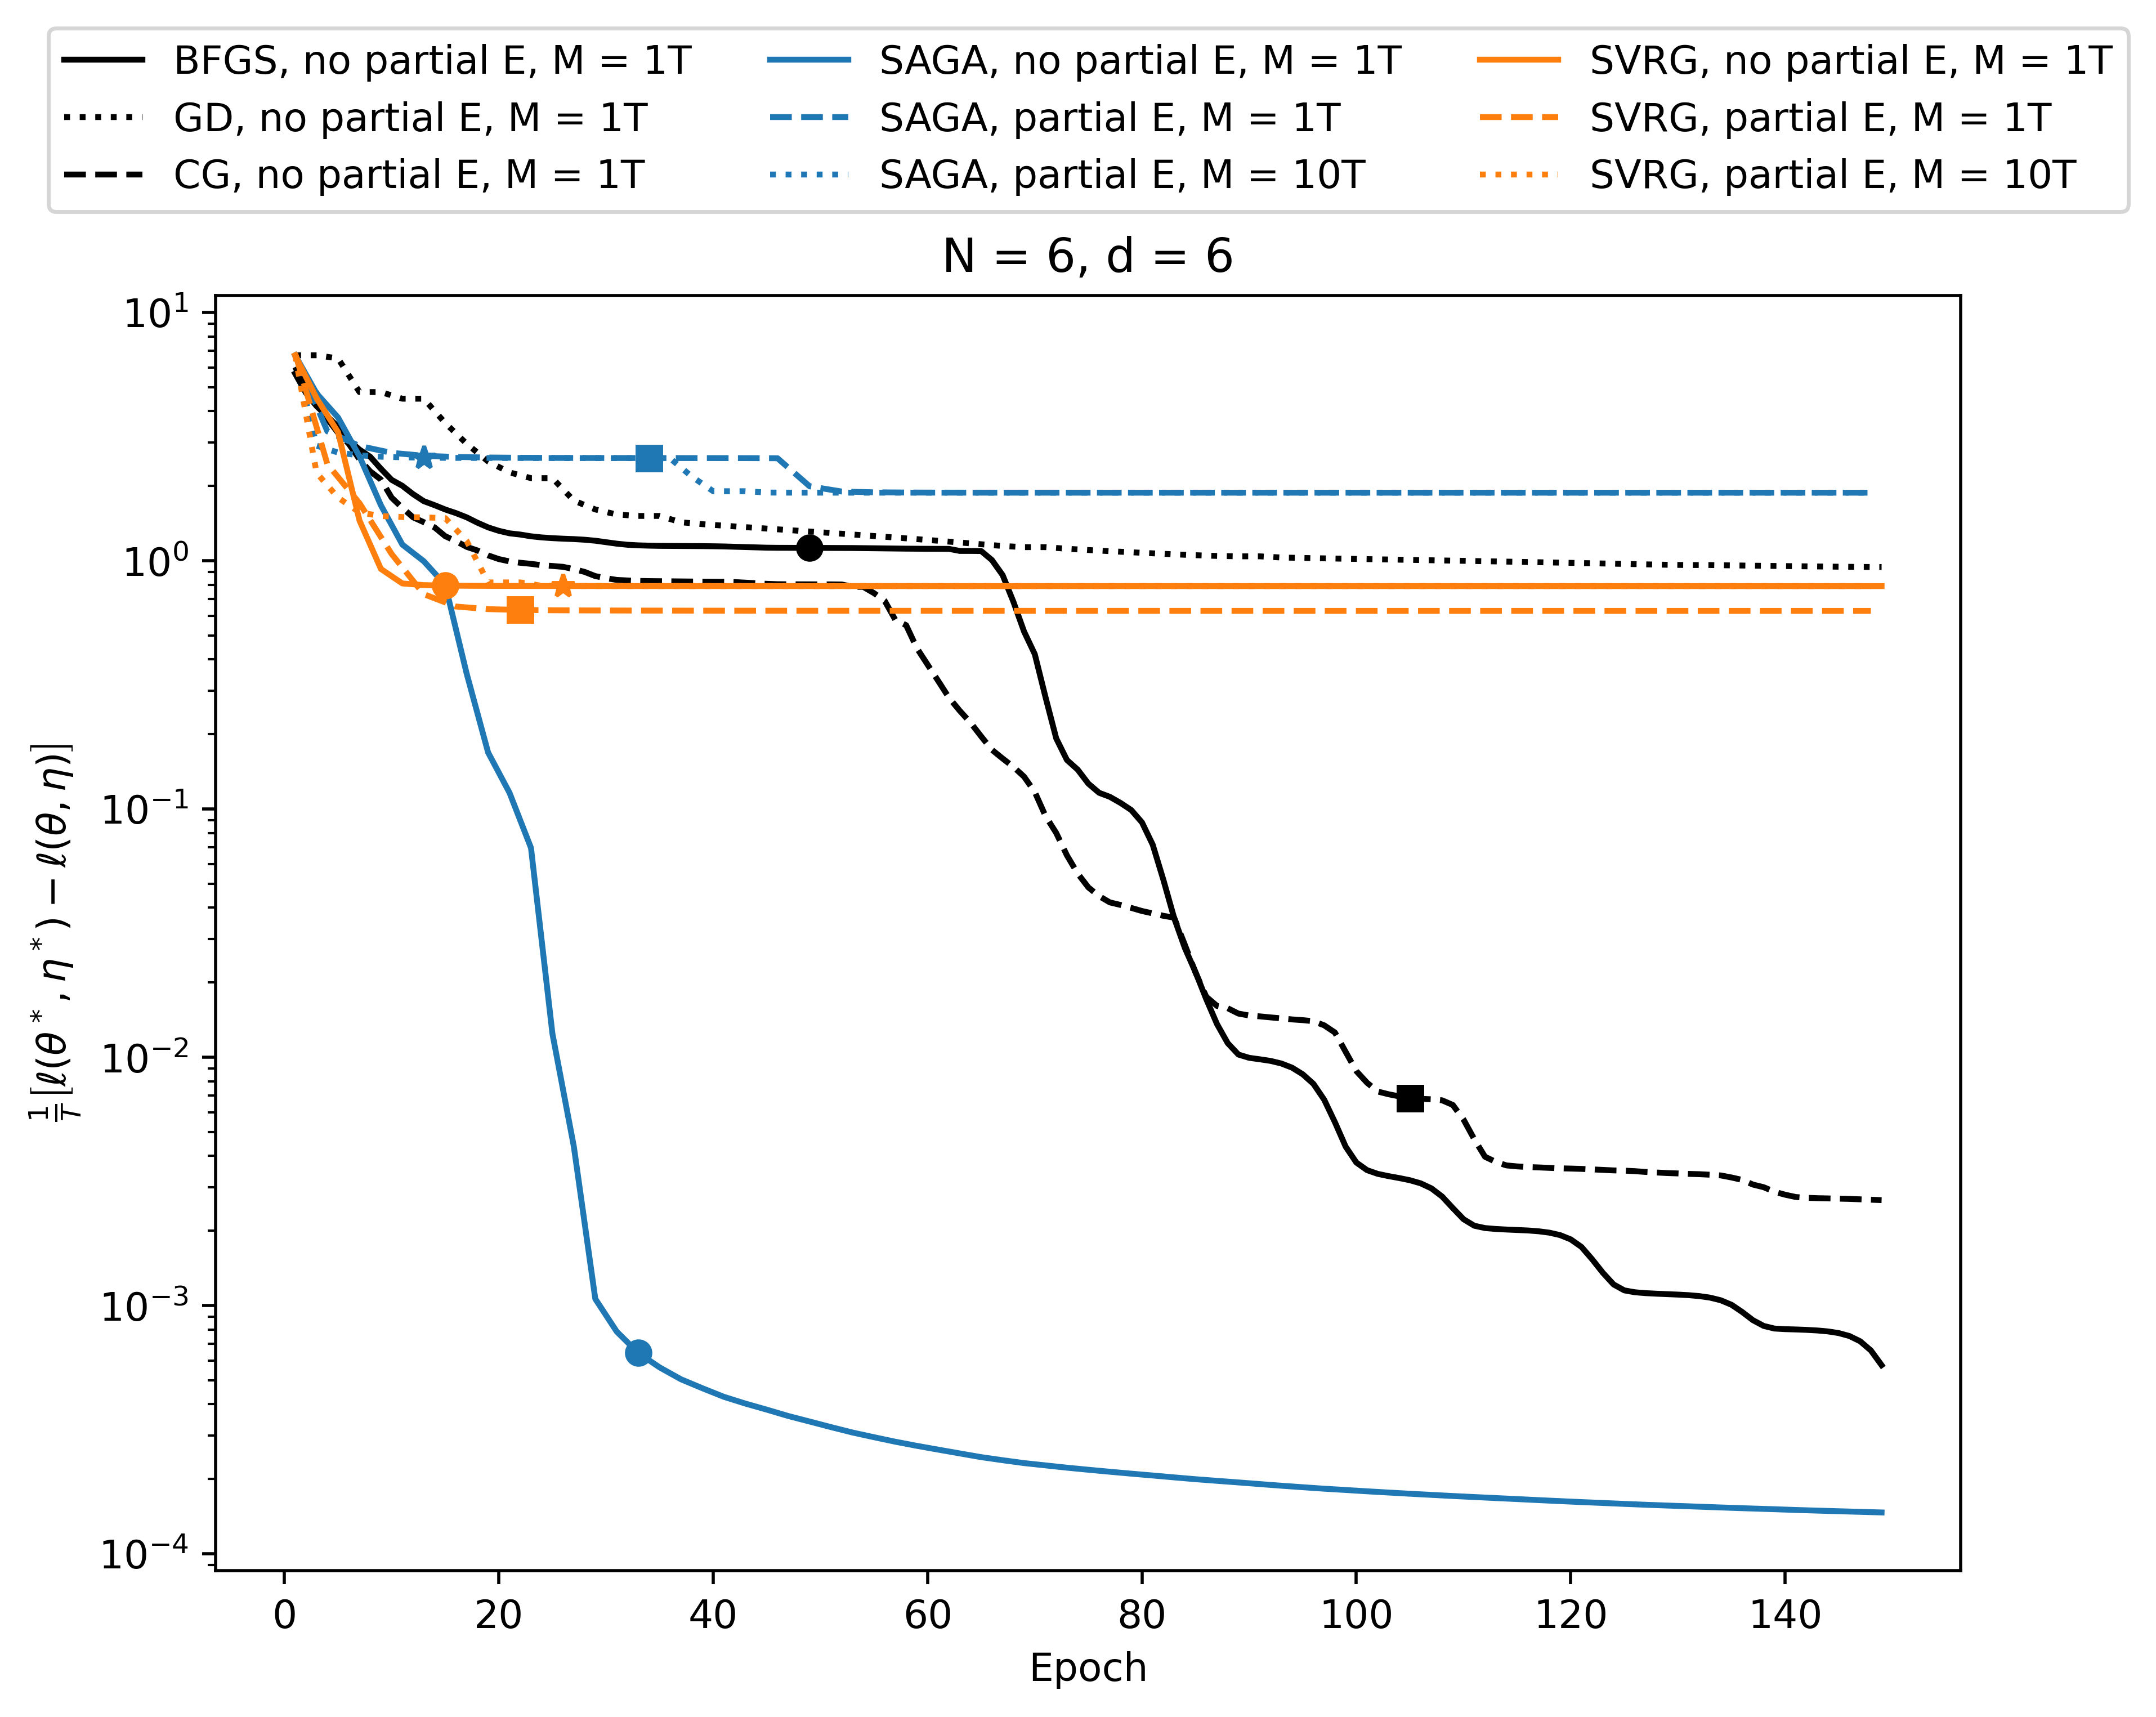
\includegraphics[width=3in]{../plt/log-like_v_epoch_T-1000-K-6-1-d-6-003.png}
    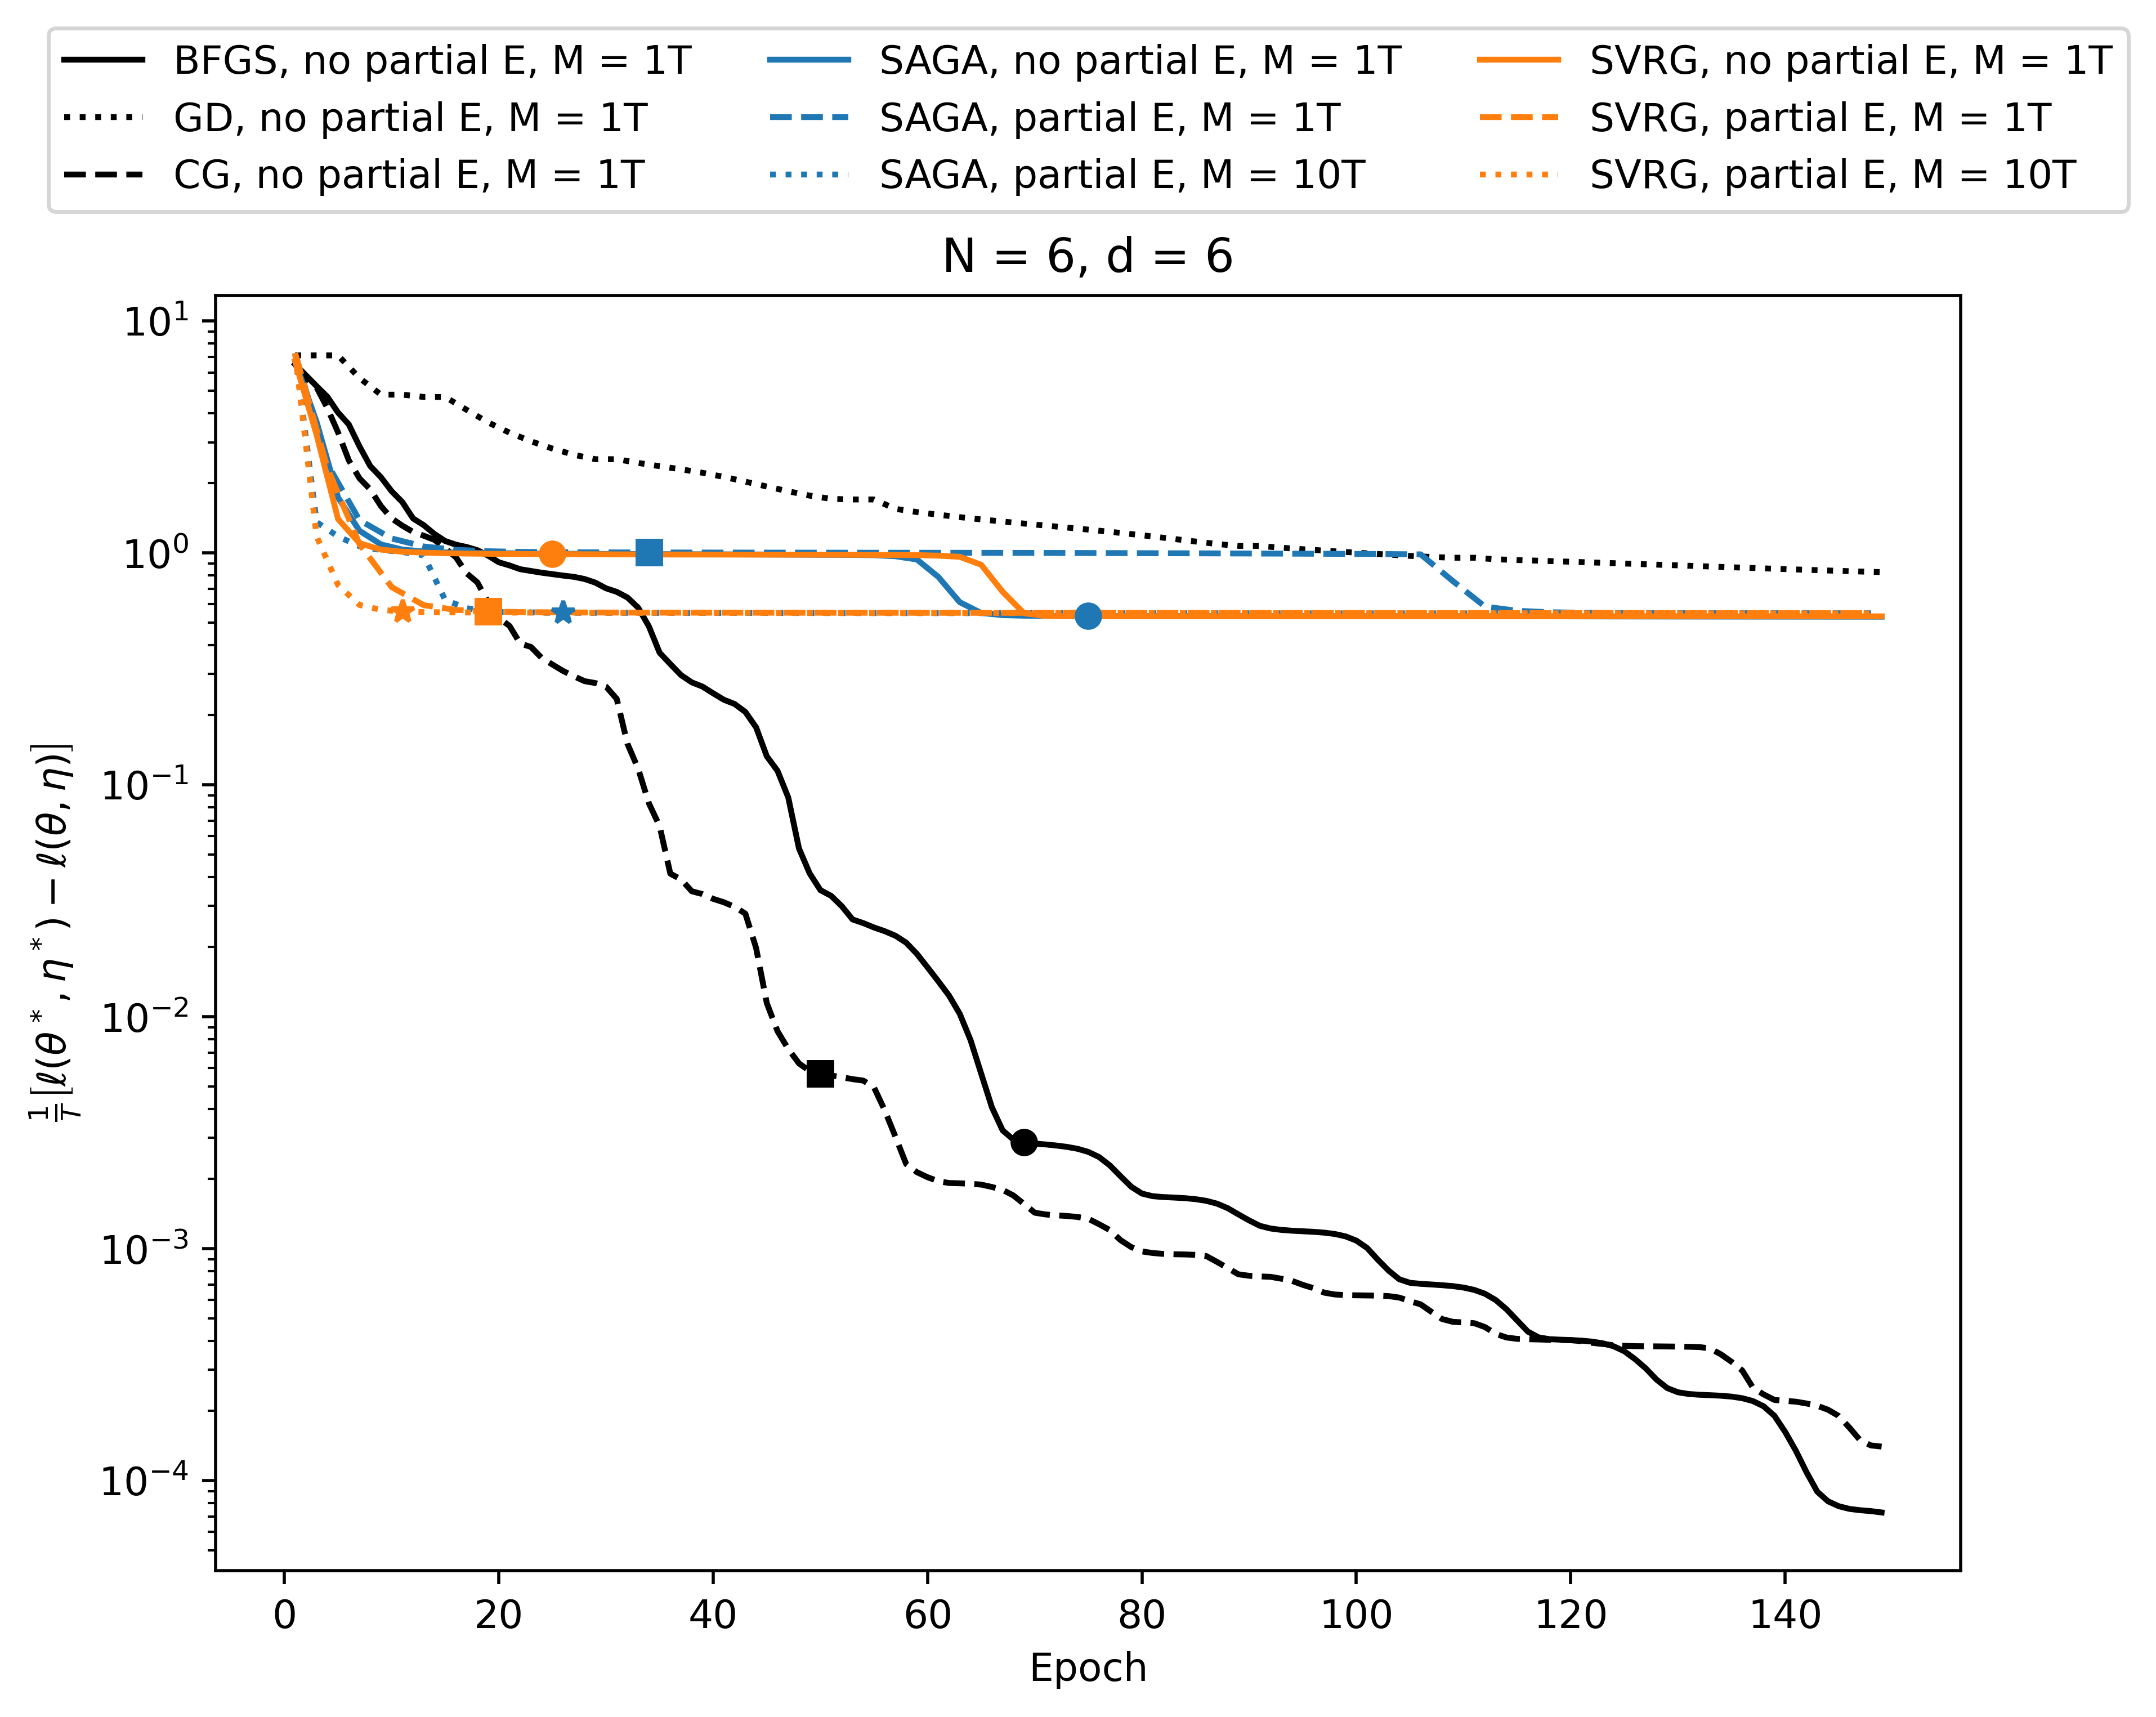
\includegraphics[width=3in]{../plt/log-like_v_epoch_T-1000-K-6-1-d-6-004.png}   
    \caption{Optimally gap between the current log-likelihood and optimal log-likelihood for the simulation studies with $T=10^{3}$, $N=6$ and $d=6$, for four different simulated data sets. One epoch represents either one full E-step, $T$ iterations with the M-step, or one gradient step for full-gradient algorithms. The y-axis is on a log-scale.}
\end{figure}

\end{document}